\documentclass[12pt]{article}
%\documentclass{nature}

% Including pdf figures
\usepackage{graphicx}
\graphicspath{ {../Plots/} }
\usepackage{pdfpages}
%really place a figure in a location
\usepackage{float}
%Overrun caption
\usepackage[CaptionAfterwards]{fltpage}
% Math stuff
\usepackage{amsmath}
\usepackage{stix}
% Bibliographies
\usepackage[numbers]{natbib}
\bibpunct{(}{)}{,}{a}{}{;} 

\usepackage[flushleft]{threeparttable}

\usepackage[font={scriptsize}]{caption}

\usepackage{lineno} %gives line numbers with \lineno command

\usepackage{setspace}
\onehalfspace

\usepackage{tikz}%for putting words on figures
\usetikzlibrary{positioning}%for relative positioning

%to rotate figures
\usepackage{rotating}
\usepackage{pdflscape}

\begin{document}

\title{Haploid Selection, Sex Ratio Bias, and Transitions Between Sex-Determination Systems}
\author{Michael F Scott$*^1$, Matthew M Osmond$*^2$, and Sarah P Otto$^2$}
\date{}
\maketitle
\noindent
$*$ These authors contributed equally to this work

\noindent
$^1$ Department of Botany, University of British Columbia, \#3529 - 6270 University Boulevard, Vancouver, BC, Canada V6T 1Z4

\noindent
$^2$ Department of Zoology, University of British Columbia, \#4200 - 6270 University Boulevard, Vancouver, BC, Canada V6T 1Z4

\noindent
email: mfscott@biodiversity.ubc.ca, mmosmond@zoology.ubc.ca

\noindent
Contributions: 

\newpage
\linenumbers
\modulolinenumbers[2]

\begin{abstract}
Sex-determination systems are remarkably dynamic; many taxa display shifts in the location of sex-determining loci or the evolution of entirely new sex-determining systems. 
Predominant theories for why we observe such transitions %in which new sex-determining systems spread by selection 
%involve sex-ratio selection or sex-specific selection (e.g., sexually antagonistic selection).
%These studies 
generally conclude that novel sex-determining systems are favoured by selection if they equalise the sex ratio or increase linkage with a sexually-antagonistic locus. 
We use population genetic models to extend these theories in two ways: 
(1) We explicitly consider how selection on very tightly sex-linked loci influences the spread of novel sex-determiners. 
We find that tightly sex-linked genetic variation can favour the spread of new sex-determination systems in which the heterogametic sex changes (XY to ZW or ZW to XY) and the new sex-determining region is less closely linked (or unlinked) to the sex-linked locus under selection, which is not predicted by previous theory. 
%With tight linkage, selection can maintain equilibria at which the allele fixed on the sex-limited chromosome (Y or W) is simultaneously favoured in the homogametic sex (XX females or ZZ males) such that heterogametic transitions (XY to ZW or ZW to XY) are favoured by selection. 
%Alternatively, a neo-W (neo-Y) locus can invade when it allows greater specialism on alleles beneficial in females (male) compared to an ancestral XX female (ZZ male), 
(2) We also consider selection upon haploid genotypes either during gametic competition (e.g., pollen/sperm competition) or meiosis (i.e., non-Mendelian segregation); selective processes that typically occur in one sex or the other. 
%As well as having sex-specific fitness consequences, haploid selection can cause the zygotic sex ratio to become biased because sex ratios are determined by the production and fertilization success of X- versus Y-bearing pollen/sperm (or Z- versus W-bearing ovules/eggs). 
%Consequently, selection for XY to ZW transitions and ZW to XY transitions can be assymetrical when linkage between the ancestral sex-determining locus and a locus under haploid selection is tight, in which case ancestral sex ratio biases can be strong.
%In addition, when linkage between the ancestral sex-determining locus and a locus under haploid selection is tight, sex ratio biases can be strong such that there is an asymmetry between invasion of ancestrally XY and ancestrally ZW systems because, e.g., haploid selection in males only causes biased zygotic sex ratios in an ancestrally XY system. 
With haploid selection, we again find that transitions between male and female heterogamety can occur even if the new sex-determining region is less closely linked to the locus under selection. 
Haploid selection in the heterogametic sex can also cause sex ratio biases, which may increase or decrease with the spread of new sex chromosomes. 
Thus, transitions between sex-determination systems cannot be simply predicted by selection to equalise the sex-ratio. 
%These results indicate that loci experiencing haploid selection can favour the evolution of new sex-determination systems. 
%These results indicate that favourable associations that develop between the ancestral sex-determining locus and selected loci can be broken during the spread of a new sex-determining region. 
%Such transitions are not possible with diploid selection alone, in which case tighter linkage increases the fitness of both males and females. 
%Notably, we find that the spread of new genetic sex-determination systems is not affected by sex ratio biases that are caused by haploid selection. 
%A surprising result given that other determinants of sex allocation typically experience strong Fisherian sex-ratio selection to equalize sex ratios. 
%Overall, we demonstrate when and how the evolution of sex determining systems is impacted by sex ratio biases resulting from haploid selection and we show that new sex-determining regions can be favoured even if they are not closely linked with a locus under selection. 
Overall, our models reveal that transitions between sex-determination systems, particularly transitions where the heterogametic sex changes, can be driven by loci in previously unexpected genomic locations that experience selection during diploid and/or haploid phases.
These results might be reflected in the lability with which sex-determination systems evolve. %and for the factors determining the phylogenetic pattern of sex-determination systems. 
\end{abstract}

%abstract word count: $\approx$ 350

\newpage

\section*{Introduction}

%CHECK THROUGHOUT: use of sex-determination SYSTEMS versus MECHANISMS. 
%CHECK THROUGHOUT: use of haploid selection, gametic selection, and meiotic drive.

Animals and angiosperms exhibit extremely diverse sex-determination systems \citep[reviewed in][]{Bull:1983vi,Charlesworth:2010it,Beukeboom:2014vb,Bachtrog:2014bx}. 
Among species with genetic sex determination of diploid sexes, some taxa have heterogametic males (XY) and homogametic females (XX), including %non-monotreme? 
mammals and most dioecious plants \citep{Ming:2011iy}; whereas other taxa have homogametic males (ZZ) and heterogametic females (ZW), including Lepidoptera and birds. 
Within several taxa, the chromosome that harbours the master sex-determining region changes. 
For example, transitions of the master sex-determining gene between chromosomes or the evolution of new master sex-determining genes have occurred in Salmonids \citep{Li:2011fm,Yano:2012di}, Diptera \citep{Vicoso:2015hf}, and \textit{Oryzias} \citep{Myosho:2012fv}.
%Presentation at evolution found neo sex chromosome in birds, doesn't seem to be published or bioRxiv yet (consider pers com.), title: A previously unknown neo-sex chromosome mediates plumage divergence and speciation in hybridizing birds Jason Sardell; Elizabeth Cooper; J. Albert C. Uy. I wonder if this is actually a fusion event though?
In addition, many gonochoric clades with genetic sex determination exhibit transitions between male (XY) and female (ZW) heterogamety, including snakes \citep{Gamble2017}, lizards \citep{Ezaz:2009tk}, eight of 26 teleost fish families \citep{Mank:2006bt}, true fruit flies \citep[Tephritids,][]{Vicoso:2015hf}, amphibians \citep{Hillis:1990gu}, the angiosperm genus \textit{Silene} \citep{Slancarova:2013dq}, the angiosperm family \textit{Salicaceae} \citep{Pucholt2015,Pucholt2017} and Coleoptera and Hemiptera \citep[][plate 2]{Beukeboom:2014vb}.
Indeed, in some cases, both male and female heterogametic sex-determination systems can be found in the same species, as exhibited by some cichlid species \citep{Ser:2010iq} and \textit{Rana rugosa} \citep{Ogata:2007jm, Miura2007}. 
In addition, multiple transitions have occurred between genetic and environmental sex-determination systems, e.g., in reptiles and fishes \citep{Conover:1987in,Mank:2006bt,Pokorna:2009ui,Ezaz:2009tk,Pen:2010kk,Holleley:2015hc}.

%NOTE: ``Bull & Charnov (1977) hypothesized that a new sex-determining gene can rapidly increase and become fixedin a population if it is linked to a gene with high adaptivevalue, and finally cause a change of the heterogametic sex.'' The Bull and Charnov paper is also the one in which the set of neutral equilibria between XY and ZW are identified (where sex ratios are equal)
%NOTE: Vuilleumier et al. 2007 also find polymorphic sex determination can be stable.

%For example, closely related species in the Medaka lineage (cite Takenhana et al. 2008) and Tilapiinae (cite Lee et al 2004, Cnaani et al 2008), citations in Beukeboom. 

%\textcolor{red}{Brief description of sex ratio adjustment and sexual antagonism theories:}

Predominant theories accounting for the spread of new sex-determination systems by selection involve fitness differences between sexes (e.g., sexually antagonistic selection) or sex-ratio selection. 
%\citet{Bull:1977wt} shows that direct selection on new sex determination loci can allow them to spread and switch between male and female heterogamety. 
\citet{vanDoorn:2007eu,vanDoorn:2010hu} show that new sex-determining loci can be favoured if they arise in closer linkage with a locus that experiences sexual antagonism. 
Tighter linkage allows a stronger favourable association to build up between a male-beneficial allele, and a neo-Y chromosome, for example. 
Such associations can favour a new master sex-determining gene on a new chromosome \citep{vanDoorn:2007eu} and can also favour a transition between male and female heterogamety \citep[e.g., a ZW to XY transition,][]{vanDoorn:2010hu}. 
However, any sexually-antagonistic loci that are more closely linked to the ancestral sex-determination locus will develop similar, favourable associations and hinder the spread of a new sex-determination system. 
%Here we extend these studies by explicitly calculating the the equilibrium allele frequencies of loci that are very tightly linked to the ancestral sex-determining region. 

The sex ratio is directly determined by the sex-determination system, and it has therefore been suggested that sex-ratio selection is a dominant force in the evolution of sex determination (e.g., \citealt{Bull:1983vi}, p 66-67; \citealt{Beukeboom:2014vb}, Chapter 7). 
`Fisherian' sex-ratio selection favours a 1:1 zygotic sex ratio when assuming that males and females are equally costly to produce \citep{Fisher:1930wy,Charnov:1982wg}.
This follows from the fact that, for an autosomal locus, half of the genetic material is inherited from a male and half from a female \citep{West:2009we}. 
Thus, if the population sex ratio is biased towards one sex, the average per-individual contribution of genetic material to the next generation from the opposite sex is greater. 
Therefore, a mutant that increases investment in the rarer sex will spread via the higher per-individual contributions made by that sex. 
%The default mode of sex-ratio selection is `Fisherian' sex-ratio selection, which favours equal investment in male and female offspring \citep[i.e., a 1:1 zygotic sex ratio when assuming that males and females are equally costly to produce,][]{Fisher:1930wy,Charnov:1982wg}. 
%Given that the sex-determination system can directly affect the sex ratio, we might expect Fisherian sex-ratio selection to influence the spread of new sex-determination systems. 
In the case of sex-chromosome evolution, \citet{Kozielska:2010vm} consider systems in which the ancestral sex chromosomes experience meiotic drive (e.g., where driving X or Y chromosomes are inherited disproportionately often), which causes sex ratios to become biased \citep{Hamilton:1967ts}. 
They find that new, unlinked sex-determining loci (masculinizing or feminizing mutations, i.e., neo-Y or neo-W loci) can then spread, which restore an even sex ratio. 

%\textcolor{red}{We add haploid selection:}
Here we use mathematical models to find the conditions under which new sex-determination systems spread when individuals experience selection at both diploid and haploid stages. 
Even in animal and plant species that have much larger and more conspicuous diploid phases than haploid phases, many loci experience significant haploid selection through gamete competition and/or meiotic drive \citep{Mulcahy:1996ha,JOSEPH:2004haa}.
We use the term `meiotic drive' to refer to the biased (non-Mendelian) segregation of genotypes during gamete production (from one parent) and the term `gametic competition' to refer to selection upon haploid genotypes within a gamete/gametophyte pool (potentially from multiple parents); the term `haploid selection' encompasses both processes. 

% from Bai et al. (2016) ``[Segregation distortion] phenomenon is commonly detected via genetic mapping and has been documented in various species, including mouse (Eversley et al., 2010; Casellas et al., 2012), Drosophila (Phadnis and Orr, 2009; Larracuente and Presgraves, 2012; McDermott and Noor, 2012), Tigriopus (Pritchard et al., 2011), rice (Koide et al., 2012; Reflinur et al., 2014; Xu et al., 2014), maize (Tang et al., 2013), and cotton (Yu et al., 2011; Hulse-Kemp et al., 2015).'' Also more in that paper that might be useful. 
%Drosophila http://www.biorxiv.org/content/early/2017/02/06/106336
Segregation distortion provides putative evidence of haploid selection and can sometimes be attributed to meiotic drive and/or gametic competition \citep{Lalanne2004,Fishman2005,Leppala2008,Leppala2013,Didion2015,Didion2016}.
Where it has been characterized, meiotic drive generally occurs either during the production of male or female gametes only \citep{Ubeda:2005gw,Lindholm:2016cw}.
Gametic competition is also typically sex specific, occurring primarily among male gametes, because there are typically many more pollen/sperm than required for fertilization.
Gametic competition may be particularly common in plants, in which 60-70\% of all genes are expressed in the male gametophyte and these genes exhibit stronger signatures of selection than random genes \citep{Borg:2009jpa,Arunkumar:2013iq,Gossmann:2014dua}.
In addition, artificial selection pressures applied to male gametophytes are known to cause a response to selection \citep[e.g.,][]{Hormaza:1996cv,Ravikumar:2003uo,Hedhly:2004iv,Clarke:2004ir}. 
A smaller proportion of genes are thought to be expressed and selected during competition in animal sperm, although precise estimates are uncertain \citep{Zheng:2001fi,JOSEPH:2004haa,Vibranovski:2010et}. 
Recent studies have demonstrated that sperm competition in animals can alter haploid allele frequencies and increase offspring fitness \citep{Immler:2014im,Alavioon2017}.

There are various ways by which genes experiencing haploid selection could influence transitions between sex-determination systems. 
If we assume that haploid selection at any particular locus predominantly occurs in one sex (e.g., meiotic drive during spermatogenesis), then such loci experience a form of sex-specific selection. 
In this respect, we might expect that haploid selection would affect transitions between sex-determination systems in a similar manner to sex-specific diploid selection \citep[as explored by][]{vanDoorn:2007eu,vanDoorn:2010hu}. 
That is, new masculinizing mutations (neo-Y chromosomes) could be favoured via associations with alleles that are beneficial in the male haploid stage. 
On the other hand, sex ratios can also become biased by linkage between the sex-determining region and a locus that harbours genetic variation in haploid fitness. 
For example, there are several known cases of sex-ratio bias caused by sex-linked meiotic drive alleles \citep[][Chapter 3]{Burt:2006} or selection among X- and Y-bearing pollen \citep{Lloyd:1974tz,Conn:1981uw,Stehlik:2005ul,Stehlik:2006to,Field:2012fd,Field:2013cc}. 
It is not immediately clear how the spread of new sex-determination systems would be influenced by the combination of sex-ratio biases and associations between haploid selected loci and sex-determining regions. 

%Perhaps longer discussion of tight sex-linkage here? e.g., mention that r=0 is a particularly significant case for sex chromosomes. 

We find that sex-ratio biases caused by haploid selection can exert Fisherian sex-ratio selection upon novel sex-determiners but that their spread is also determined by selection on genetically-associated alleles. 
%Indeed, it is only when haploid-selected loci are tightly linked to the ancestral sex-determining region (and so sex-ratio biases are initially large) that we see an asymmetry between selection for XY to ZW transitions and ZW to XY transitions (e.g., because haploid selection in males only causes biased zygotic sex ratios in an ancestrally XY system).
Consequently, Fisherian sex ratio selection does not dominate and it is possible for selection on linked alleles to drive turnover between sex-determining systems despite causing increases in sex-ratio bias. 
In addition to considering haploid selection, another novel development in our model is that we consider loci that are in very tight linkage with the ancestral sex-determining region.
We show that transitions between male and female heterogamety can then evolve despite the fact that the neo-sex-determining locus is less closely linked to a locus under selection and therefore disrupts favourable ancestral associations between sex and the alleles favoured in that sex.
%Such transitions are not favoured in models lacking tight linkage and/or haploid selection. 
%Secondly, we allow sex-specific haploid selection to occur on a locus in tight or loose linkage with the ancestral sex-determining region. 
%In addition, when linkage between the ancestral sex-determining locus and a locus under haploid selection is tight, sex ratio biases can be strong such that there is an asymmetry between invasion of ancestrally XY and ancestrally ZW systems because, e.g., haploid selection in males only causes biased zygotic sex ratios in an ancestrally XY system. 

%%%%%%%%%%%%%%%%%%%%%%%%%%
\section*{Model}
%%%%%%%%%%%%%%%%%%%%%%%%%

%\textcolor{red}{Change all  $\alpha^\Hermaphrodite$ to $(1+\alpha_{\Delta}^\Hermaphrodite)$.}
%\textcolor{blue}{I've attempted this everywhere except in the recursions (S.1), which seem more natural with $\alpha$'s. I've run into trouble in equation S.8c,d -- I think we should check the Mathematica results to be sure we haven't made a typo. This also introduced an extra 1/2 in S.6c,d that might need to be explained.}
%\textcolor{red}{hmm, not sure. This was an idea from Sally, I think in response to terms like $2 \alpha^\Hermaphrodite$ and $2(1-\alpha^\Hermaphrodite)$. It's possible that it makes other equations less easy to understand. My previous (not explained) logic was to use $w$ and $\alpha$ for strong selection and $s$, $t$, and $\alpha_\Delta$ for weak selection. Just to check, I should have written $\alpha^\Hermaphrodite=(1+\alpha_{\Delta}^\Hermaphrodite)/2$, maybe that's where the factors of $1/2$ come from?}
%\textcolor{blue}{shoot, i may have changed too much (i.e. strong selection too), but i did use the correct transformation. still, the form of S.8c,d seems wrong. I'll double check it. CANT FIND ANY ERRORS YET STILL HAVE A "2" IN S.8c. These 2s reappear in S.9 and S.10, always with $W_{AA}$.}

%\textcolor{red}{Switch between $\rho$ and $\rho$ in all places because $\rho$ is used for double recombination events.}
%\textcolor{blue}{I think we need a different variable given the $\rho$ terms in the characteristic polynomial. Also, where is $\rho$ used for double recombination? In other papers? Here $\rho$ is the probability of an odd number of cross-overs between the SDR and M loci.}
%\textcolor{red}{Good point, not sure what's best for \textbf{the-term-formerly-known-as-$\rho$}. Yeah, Sally's written comment was something like ``$\rho$ is semi-standard notation for double recombination so it's use as a recombination rate might be confusing''.}

%\textcolor{red}{Change $\zeta$ to represent zygotic sex ratio of males, consistent with $q$ and figures.}

%genetic system
We consider transitions between ancestral and novel sex-determining systems using a three-locus model, each locus having two alleles. 
Locus \textbf{X} is the ancestral sex-determining region, with alleles $X$ and $Y$ (or $Z$ and $W$).
Locus \textbf{A} is a locus under selection, with alleles $A$ and $a$.
Locus \textbf{M} is a novel sex-determining region, at which the null allele ($M$) is initially fixed in the population such that sex of zygotes is determined by the genotype at the ancestral sex-determining region, \textbf{X}; $XX$ genotypes become females and $XY$ become males (or $ZW$ become females and $ZZ$ become males). 
To evaluate the evolution of new sex-determination systems, we consider the invasion, fixation, maintenance, and/or loss of novel sex-determining alleles ($m$) at the \textbf{M} locus. 
%We only do invasion analytically though (is this sentence still ok?)
We assume that the \textbf{M} locus is epistatically dominant over the \textbf{X} locus such that zygotes with at least one $m$ allele develop as females with probability $k$ and as males with probability $1-k$, regardless of the \textbf{X} locus genotype.
With $k=0$, the $m$ allele is a masculinizer (i.e., a neo-Y) and with $k=1$ the $m$ allele is a feminizer (i.e., a neo-W).
With intermediate $k$, we can interpret $m$ as an environmental sex determination (ESD) allele, such that zygotes develop as females in a proportion ($k$) of the environments they experience. 
%We also analyze a model of maternally-controlled environmental sex-determination, where mothers with at least one $m$ allele produce daughters with probability $k$. 

%life-cycle
In each generation, we census the genotype frequencies in male and female gametes/gametophytes (hereafter gametes) before gametic competition. 
A full description of our model, including recursion equations, is given in the Appendix. 
First, competition occurs among male gametes (sperm/pollen competition) and among female gametes (egg/ovule competition) separately. 
Selection during gametic competition depends on the \textbf{A} locus genotype, relative fitnesses are given by $w_A^\Hermaphrodite$ and $w_a^\Hermaphrodite$ ($\Hermaphrodite \in \{\female,\male\}$; see table \ref{tab:fitnesstable}). %$w_{A}^\male$ and $w_{a}^\male$ for male gametes and $w_{A}^\female$ and $w_{a}^\female$ for female gametes, see table \ref{tab:fitnesstable}. 
We assume that all gametes compete for fertilization during gametic competition, which assumes a polygamous mating system. 
Gametic competition in monogamous mating systems is, however, equivalent to meiotic drive in our model (described below), as both only alter the frequency of gametes produced by heterozygotes. 
After gametic competition, random mating occurs between male and female gametes.
The resulting zygotes develop as males or females, depending on their genotypes at the \textbf{X} and \textbf{M} loci. %(and the \textbf{M} genotype of their mother in the case of maternal control).
Diploid males and females then experience selection, with relative fitnesses $w_{AA}^{\Hermaphrodite}$, $w_{Aa}^{\Hermaphrodite}$, and $w_{aa}^{\Hermaphrodite}$. %where $g$ is the diploid genotype at the \textbf{A} locus ($g \in \{AA, Aa, aa\}$).  
%Diploids compete with others of the same sex, where selection depends on the sex of the individual and its genotype at the \textbf{A} locus.
The next generation of gametes is produced by meiosis, during which recombination and sex-specific meiotic drive can occur. 
Recombination (i.e., an odd number of cross-overs) occurs between loci \textbf{X} and \textbf{A} with probability $r$, between loci \textbf{A} and \textbf{M} with probability $R$, and between loci \textbf{X} and \textbf{M} with probability $\rho$.
Any linear order of the loci can be modelled with appropriate choices of $r$, $R$, and $\rho$ (see Table \ref{tab:chisubstitutions}). 
Individuals that are heterozygous at the \textbf{A} locus may experience meiotic drive; a gamete produced by $Aa$ heterozgotes of sex $\Hermaphrodite$ bear allele $A$ with probability $\alpha^\Hermaphrodite$. 
Thus, the \textbf{A} locus can experience sex-specific gametic competition, diploid selection, and/or meiotic drive. 



\begin{table}[ht]
\centering
\smallskip
\caption{Relative fitness of different genotypes in sex $\Hermaphrodite \in \{\female,\male\}$}
\begin{tabular}{l c }
\hline\hline
  Genotype & Relative fitness during gametic competition \\ [0.5ex] \hline
  A & $w_{A}^\Hermaphrodite = 1+t^\Hermaphrodite$ \\
  a & $w_{a}^\Hermaphrodite = 1$ \\ [0.5ex] \hline
  Genotype & Relative fitness during diploid selection \\ [0.5ex] \hline
  AA & $w_{AA}^\Hermaphrodite = 1+ s^\Hermaphrodite$ \\
  Aa & $w_{Aa}^\Hermaphrodite = 1+h^\Hermaphrodite s^\Hermaphrodite$ \\
  aa & $w_{aa}^\Hermaphrodite = 1$ \\ [0.5ex] \hline
  Genotype & Transmission during meiosis in $Aa$ heterozygotes \\ [0.5ex] \hline
  A & $\alpha^\Hermaphrodite=1/2+\alpha_{\Delta}^{\Hermaphrodite}/2$ \\
  a & $1-\alpha^\Hermaphrodite=1/2-\alpha_{\Delta}^{\Hermaphrodite}/2$ \\
  \hline \hline
  \label{tab:fitnesstable}
 \end{tabular}
\end{table}

%Info moved above
%what were going to do, briefly
%With allele $M$ fixed at the \textbf{M} locus, sex is determined by locus \textbf{X} and an equilibrium is reached at locus \textbf{A}. %where, importantly, locus \textbf{A} can be stably polymorphic. %the dynamics can be described by the frequency of $A$ in gametes/gametophytes from the homogametic sex and the frequencies of $A$ in the two types of gametes/gametophytes from the heterogametic sex.
%We then examine the ability of a rare, novel sex-determiner, $m$, to increase in frequency from this equilibrium.
%Numerical simulations are used to examine when an invading mutation goes to fixation.

%%%%%%%%%%%%%%%%%%%%%%%%%%
\section*{Results}
%%%%%%%%%%%%%%%%%%%%%%%%%

The model outlined above describes both ancestrally-XY and ancestrally-ZW sex-determination systems if we relabel the two sexes as being ancestrally `heterogametic' or ancestrally `homogametic'. 
Without loss of generality, we primarily refer to the ancestrally heterogametic sex as male and the ancestrally homogametic sex as female.
That is, we describe an ancestral XY sex-determination system but our model is equally applicable to an ancestral ZW sex-determination system (relabelling the ancestrally-heterogametic sex as female and the ancestrally-homogametic sex as male). 

%\subsection*{Turnover between sex-determination systems} 

\subsubsection*{Generic invasion by a neo-Y or neo-W}

The evolution of a new sex-determination system requires that a rare mutant allele at the novel sex-determining locus, $m$, increases in frequency when rare. 
The spread of a rare mutant $m$ at the \textbf{M} locus is determined by the leading eigenvalue, $\lambda$, of the system of eight equations describing the frequency of eggs and sperm carrying the $m$ allele in the next generation (equations \ref{eq:recursions}). %, evaluated at the above equilibrium.
%Thus, the system describing the change in frequency of the $m$ allele consists of eight recursion equations. 
This system simplifies substantially in a number of cases of interest. 
Dominant neo-Y (when $k=0$) or neo-W alleles (when $k=1$) are only found in male diploids (neo-Y) or female diploids (neo-W) such that their growth rate ultimately depends only on the change in frequency of $m$-bearing gametes produced by males or by females, respectively. 
Furthermore, if the $m$ allele is fully epistatically dominant over the ancestral sex-determining system, phenotypes are not affected by the genotype at the ancestral sex-determining region (\textbf{X} locus). 
Thus, the invasion of rare dominant neo-Y or neo-W alleles is determined by the largest eigenvalue that solves a quadratic characteristic polynomial,
%\textcolor{red}{Mention the possibility that the other roots yield the leading eigenvalue somewhere.}
%\textcolor{blue}{following the logic above, it seems like we say we go from 8 eqns to 4 eqns by considering only one sex, and then from 4 eqns to 2 eqns by ignoring the ancestral SD allele. why then do we have the two quadratic problem? (b/c the $m$ alleles can arise in either sex?)}
$\lambda^2+ b \lambda + c =0$ \textcolor{blue}{(see Appendix for a discussion of other roots - or Sally's proof!)}.
%\begin{equation}
%\lambda^2+ b \lambda + c =0
%\label{eq:charpoly_neoY}
%\end{equation}
%
%\noindent
%where $b$ is the average of the growth rates of the two haplotypes that carry the $m$ allele ($mA$ and $ma$), $b=(\lambda_{mA}+\lambda_{ma})/2$, and $c$ also involves the fitness of $m$ alleles when they recombine onto the other \textbf{A} background in a heterozygote, $c=\lambda_{mA}\lambda_{ma}+\chi_{mA}\chi_{ma}$ (see table \ref{tab:haplotype_growth}).
%Here, $b= - (\lambda_{mA} + \lambda_{ma})$ and $c = \lambda_{mA} \lambda_{ma} -\chi_{mA} \chi_{ma}$, where $\lambda_{mi}$ is the (multiplicative) growth rate of mutant haplotypes on background $i\in\{A,a\}$, accounting for loss due to recombination, and $\chi_{mi}$ is the rate of addition of mutant haplotypes onto background $i\in\{A,a\}$ due to recombination (see table \ref{tab:haplotype_growth}).
Here, $b= - (\lambda_{mA} + \lambda_{ma})+(\chi_{mA} + \chi_{ma})$ and $c = (\lambda_{mA}-\chi_{mA}) (\lambda_{ma}-\chi_{ma}) -\chi_{mA} \chi_{ma}$, where $\lambda_{mi}$ is the multiplicative growth rate of mutant haplotypes on background $i\in\{A,a\}$, without accounting for loss due to recombination, and $\chi_{mi}$ is the rate at which mutant haplotypes on background $i\in\{A,a\}$ recombine onto the other \textbf{A} locus background in heterozygotes (see Table \ref{tab:haplotype_growth}).
The $\lambda_{mi}$ and $\chi_{mi}$, and thus the spread of the mutant $m$ allele, depend on the frequency of alleles at the \textbf{A} and \textbf{X} loci in the ancestral population. 
In the ancestral population, it is convenient to follow the frequency of the $A$ allele among female gametes (eggs), $p^\female_X$, and among X-bearing, $p^\male_X$, and among Y-bearing, $p^\male_Y$, male gametes (sperm/pollen). 
We also track the fraction of male gametes that are Y-bearing, $q$, which may deviate from $1/2$ due to meiotic drive in males. 
We will consider only equilibrium frequencies of alleles, $\hat{p}^\Hermaphrodite_i$, and Y-bearing male gametes, $\hat{q}$, to ensure the eigenvalues of the invasion analysis are valid.  

%\textcolor{red}{I now remove the zygotic sex ratio $\zeta$ from the mean fitnesses. The mean fitnesses will have to be adjusted in a corresponding way.}
%
%\textcolor{red}{CHECK: DO THE HAPLOID MEAN FITNESSES HAVE TO BE IN THE DENOMINATOR? i think so, based on definitions in table S.2 (mmo)}

% as there are now two 2s in the lambdas of table 2. perhaps the 2 in the denominator is needed because the frequency of males sums to one as does the frequency of females?}

\begin{threeparttable}[ht]
\centering
\smallskip
%\caption{Parameters determining invasion (equation \ref{eq:charpoly_neoY}) for neo-Y or neo-W alleles}
\caption{Parameters determining invasion of mutant neo-Y and neo-W alleles into an ancestrally XY system}
\begin{tabular}{l}
\hline\hline
   \noalign{\vskip 0.5ex}
   neo-Y ($k=0$) \\ [0.5ex] \hline \noalign{\vskip 1ex}
  $\lambda_{mA} = \left( 2 \zeta \right)^{-1} \left[\hat{p}_X^\female w_{A}^{\female} w_{A}^{\male} w_{AA}^{\male} + (1-\hat{p}_X^\female) w_{a}^{\female} w_{A}^{\male} w_{Aa}^{\male} (1+\alpha_{\Delta}^{\male}) \right]/ \left( \bar{w}_H^\female \bar{w}_H^\male \bar{w}^\male \right) $\\ [0.5ex] \noalign{\vskip 0.5ex}
  $\lambda_{ma} = \left( 2 \zeta \right)^{-1} \left[(1-\hat{p}_X^\female) w_{a}^{\female} w_{a}^{\male} w_{aa}^{\male} + \hat{p}_X^\female w_{A}^{\female} w_{a}^{\male} w_{Aa}^{\male}(1 - \alpha_{\Delta}^{\male}) \right]/ \left( \bar{w}_H^\female \bar{w}_H^\male \bar{w}^\male \right) $ \\ [0.5ex] \noalign{\vskip 0.5ex}
  $\chi_{mA} = R \left( 2 \zeta \right)^{-1} \left[ (1-\hat{p}_X^\female) w_{a}^{\female} w_{A}^{\male} w_{Aa}^{\male} (1+\alpha_{\Delta}^{\male}) \right]/  \left( \bar{w}_H^\female \bar{w}_H^\male \bar{w}^\male \right)   $\\ [0.5ex] \noalign{\vskip 0.5ex}
  $\chi_{ma} = R \left( 2 \zeta \right)^{-1} \left[   \hat{p}_X^\female w_{A}^{\female} w_{a}^{\male} w_{Aa}^{\male} (1 - \alpha_\Delta^{\male}) \right]/ \left( \bar{w}_H^\female \bar{w}_H^\male \bar{w}^\male \right)  $\\ [1ex] \hline 
  \noalign{\vskip 0.5ex}
  neo-W ($k=1$) \\ [0.5ex] \hline \noalign{\vskip 1ex}
  $\lambda_{mA} = \left[ 2 (1 - \zeta) \right]^{-1} \left[ \bar{p}^{\male} w_{A}^{\male} w_{A}^{\female} w_{AA}^{\female}+(1-\bar{p}^{\male}) w_{a}^{\male} w_{A}^{\female} w_{Aa}^{\female}(1+\alpha_{\Delta}^{\female})\right]/ \left(\bar{w}_H^\female \bar{w}_H^\male \bar{w}^\female \right) $ \\ [0.5ex] \noalign{\vskip 0.5ex}
  $\lambda_{ma} = \left[ 2 (1 - \zeta) \right]^{-1} \left[ (1-\bar{p}^{\male}) w_{a}^{\male} w_{a}^{\female} w_{aa}^{\female}+\bar{p}^{\male} w_{A}^{\male} w_{a}^{\female} w_{Aa}^{\female}(1-\alpha_{\Delta}^{\female})\right] / \left(\bar{w}_H^\female \bar{w}_H^\male \bar{w}^\female \right) $ \\ [0.5ex] \noalign{\vskip 0.5ex}
  $\chi_{mA} = R \left[ 2 (1 - \zeta) \right]^{-1} \left[ (1-\bar{p}^{\male}) w_{a}^{\male} w_{A}^{\female} w_{Aa}^{\female} (1+\alpha_{\Delta}^{\female}) \right] / \left(\bar{w}_H^\female \bar{w}_H^\male \bar{w}^\female \right)  $\\ [0.5ex] \noalign{\vskip 0.5ex}
  $\chi_{ma} = R \left[ 2 (1 - \zeta) \right]^{-1} \left[ \bar{p}^{\male} w_{A}^{\male} w_{a}^{\female} w_{Aa}^{\female} (1-\alpha_{\Delta}^{\female}) \right] / \left(\bar{w}_H^\female \bar{w}_H^\male \bar{w}^\female \right) $\\ [1ex] 
  \hline \hline 
   \end{tabular}
      \begin{tablenotes}
      \scriptsize
      \item $\bar{p}^{\male}=(1-\hat{q})\hat{p}_X^\male + \hat{q}\hat{p}_Y^\male$ is the average frequency of the $A$ allele among X- and Y-bearing male gametes.
%      \item $R$ is the probability of recombination between loci \textbf{A} and \textbf{M}.
      \item $\zeta$ is the zygotic sex ratio (fraction male)
      \item $\bar{w}^\Hermaphrodite$ is the mean fitness of diploids of sex $\Hermaphrodite$, see Table \ref{tab:meanfitnesses}
      \item $\bar{w}_H^\Hermaphrodite$ is the mean fitness of haploids from sex $\Hermaphrodite$, see Table \ref{tab:meanfitnesses}
%      \item $\bar{w}_H^\female = p_X^\female w_A^\female + (1-p_X^\female) w_a^\female$ is the mean fitness of female gametes during gametic competition
%      \item $\bar{w}_H^\male = \bar{p}^{\male} w_A^\male + (1-\bar{p}^{\male}) w_a^\male$ is the mean fitness of male gametes during gametic competition
%       \item $\bar{w}^\female = \{ p_X^\female w_A^\female (1-q) p_X^\male w_A^\male w_{AA}^\female + (1 - p_X^\female) w_a^\female (1-q) p_X^\male w_A^\male w_{Aa}^\female + p_X^\female w_A^\female (1-q) (1 - p_X^\male) w_a^\male w_{Aa}^\female + (1-p_X^\female) w_a^\female (1-q) (1 - p_X^\male) w_a^\male w_{aa}^\female \} / \{ \bar{w}_H^\female \bar{w}_H^\male\}$ is the mean fitness of females during diploid competition
%       \item $\bar{w}^\male = \{ p_X^\female w_A^\female q p_Y^\male w_A^\male w_{AA}^\male + (1 - p_X^\female) w_a^\female q p_Y^\male w_A^\male w_{Aa}^\male + p_X^\female w_A^\female q (1 - p_Y^\male) w_a^\male w_{Aa}^\male + (1-p_X^\female) w_a^\female q (1 - p_Y^\male) w_a^\male w_{aa}^\male \} / \{ \bar{w}_H^\male \bar{w}_H^\male\}$ is the mean fitness of males during diploid competition
    \end{tablenotes}
  \label{tab:haplotype_growth}
\end{threeparttable}
\\

%We are particularly concerned with the conditions under which a rare neo-sex-determining allele increases in frequency, which occurs when the largest eigenvalue, $\lambda$, is greater than one. 
%If one or both of $\lambda_{mA}$ and $\lambda_{ma}$ are greater than one, indicating that at least one haplotype increases in frequency faster than recombination breaks it apart, invasion will always occur ($\lambda>1$). 
%Otherwise, invasion requires
%\begin{equation}
%(\lambda_{mA}-1)(\lambda_{ma}-1) - \chi_{mA} \chi_{ma}<0.
%\end{equation}

We are particularly concerned with the conditions under which a rare neo-sex-determining allele increases in frequency, which occurs when the largest eigenvalue, $\lambda$, is greater than one. 
%If the average change in frequency of the two haplotypes that carry the $m$ allele ($Am$ and $am$) is positive, invasion will always occur, i.e., if $(\lambda_{mA} + \lambda_{ma})/2 > 1$ then $\lambda > 1$. 
Given the characteristic polynomial $f(\lambda)=\lambda^2+b\lambda+c$ and the Perron-Forbenius theorem (guaranteeing that the leading eigenvalue is positive, unique, and real), at least one solution to $f(\lambda)=0$ is greater than one when the polynomial has a negative slope or negative value at $\lambda=1$ ($f'(1) = 2 + b < 0$ or $f(1) = 1 + b + c < 0$).
% $(\lambda_{mA} - \chi_{mA}) + (\lambda_{ma} -  \chi_{ma}) > 2$.
%In words, the neo-sex-determining allele will certainly spread when the average change in its frequency, taking into account that recombination breaks up mutant $mi$ haplotypes (at rate $\chi_{mi}$) but ignoring the fact that recombination also creates mutant haplotypes, is positive.
%When this does not hold ($2+b>0$), we can still have one $\lambda$ greater than one when 1 + b + c < 0.
Regardless the rate of recombination, at least one of these conditions is true if both haplotypes can spread ($\lambda_{mA}, \lambda_{ma} > 1$) and neither can be true if neither haplotype can spread ($\lambda_{mA}, \lambda_{ma} < 1$). 
%If both haplotypes can spread ($\lambda_{mA}, \lambda_{ma} > 1$), this condition becomes $\chi_{mA}/(\lambda_{mA} - 1) + \chi_{ma}/(\lambda_{ma} -  1) > 1$.
If only one haplotype can spread then the new sex-determining allele increases in frequency on one \textbf{A} background and declines on the other.
%Considering an alternative polynomial $g(\lambda)=\lambda^2+b\lambda+C$, with $C=(\lambda_{mA}-\chi_{mA})(\lambda_{ma}-\chi_{ma})$, we have $g(\lambda)=(\lambda_{mA} - \chi_{mA} - \lambda)(\lambda_{ma} - \chi_{ma} - \lambda)$ and, since $\chi_{mi}\leq0$, we also have $f(\lambda)<g(\lambda)$.
%Thus if $f'(1)=2+b<0$ and only one $\lambda_{mi}$ is greater than one we are guaranteed that $f(1)<g(1)<0$.
%Therefore, if only one haplotype can spread, invasion is completely determined by $f(1)<0$, which in this case can be rewritten
Invasion then occurs if
\begin{equation}\label{eq:lambdasGen}
%\frac{\chi_{mA}}{\lambda_{mA}-1}+\frac{\chi_{ma}}{\lambda_{ma}-1}>0.
\chi_{ma}/\left(\lambda_{ma}-1\right) + \chi_{mA}/\left(\lambda_{mA}-1\right) < 1.
\end{equation}
\noindent For example, if we assume that only the $mA$ haplotype has a positive growth rate ($\lambda_{ma}<1<\lambda_{mA}$), the first term on the left-hand side of \eqref{eq:lambdasGen} is negative and invasion requires that the growth rate of $mA$ haplotypes ($\lambda_{mA}-1$) and the rate at which they are produced by recombination in $ma$ haplotypes ($\chi_{ma}$) are sufficiently large relative to the rate of decline of $ma$ haplotypes ($1-\lambda_{ma}$) and the rate of loss of $mA$ haplotypes due to recombination ($\chi_{mA}$).
%\textcolor{blue}{i've updated this section with the correct $\lambda$ and $\chi$ terms. still a bit funny that not guaranteed invasion when both lambdas greater than one, and when both are greater than one then the condition above, (1), has the inequality flipped, which makes no sense (no invasion if no recombination despite both haplotypes growing). perhaps i made a mistake somewhere? see turnoverhomhet.nb}
%In other words, invasion requires that the average growth rate of the two haplotypes, weighted by the rates they are created by recombination, is positive.
%the number of recombinants from the fitter $mA$ haplotypes is larger than that of the less fit $ma$ haplotypes, relative to their growth rates. 

Table \ref{tab:haplotype_growth} illustrates a number of key points about the invasion of neo-Y and neo-W mutations. 
First, Fisherian sex-ratio selection will favour the spread of a neo-Y if the ancestral zygotic sex ratio is biased towards females, $\zeta<1/2$ (i.e., the first factor of the $\lambda_{mi}$ is greater than one for a neo-Y and less than one for a neo-W).
However, the spread of a neo-Y (neo-W) also depends on the male (female) fitness of associated alleles (terms involving equilibrium allele frequencies, $\hat{p}$'s). %, see terms in curly brackets. 
Second, invasion by a neo-Y (neo-W) allele does not directly depend on the fitness of female (male) diploids (for a given set of equilibrium allele frequencies).
%involve any female (male) diploid selection terms ($w_{g}^{\female}$)
This is because a dominant neo-Y (neo-W) is always found in males (females), and therefore the frequency of the neo-Y (neo-W) allele, $m$, only changes in males (females). 
%Therefore, invasion by a neo-Y allele does not involve any female diploid selection terms ($w_{g}^{\female}$). 
%Similarly, invasion by a neo-W is driven by the fitness of female gametes and diploids and does not involve any direct selection in male diploids. 
Finally, invasions by a neo-Y and a neo-W are qualitatively different.
This is because a gamete with the ancestral- or neo-Y always pairs with a female gamete containing an X, and both develop into males.
By contrast, a gamete with a neo-W can pair with an X or Y male gamete, developing into a female, while female gametes without the neo-W can become female (when paired with X) or male (when paired with Y).
Consequently, the types of females produced differ in the frequency of $A$ alleles they obtain from mating.
%\textcolor{blue}{nice}
%the diploid fitness terms in Table \ref{tab:haplotype_growth} are weighted by the probability of producing those genotypes through matings with gametes of the opposite sex. 
%For example, matings between a neo-Y-bearing male gamete and an $A$-bearing female gamete occur with probability $\hat{p}_X^\female w_{A}^{\female}/\bar{w}_{H}^{\female}$. 
%This is the same probability that an ancestral-Y-bearing male gamete will inherit an $A$ allele via mating with a female gamete. 
%On the other hand, 
%The probability that a neo-W bearing female gamete mates with an $A$-bearing male gamete is $\bar{p}^{\male} w_{A}^{\male}/\bar{w}_{H}^{\male}$, where $\bar{p}^{\male}=\hat{p}_Y^\maleq+\hat{p}_X^\male(1-q)$ is the frequency of the A allele among both X- and Y-bearing male gametes. 
%That is, in the case of a neo-W, female diploids can result from matings with either an X-bearing or a Y-bearing sperm, resulting in zygotes that will develop as females. 
%However, females that do not carry the neo-W only result from matings with X-bearing sperm. 
%Therefore, eggs with and without a neo-W can differ in the frequency of $A$ alleles they obtain from matings with male gametes. 
%Invasions by a neo-Y and a neo-W differ in this respect because sperm with or without a neo-Y allele both mate with X-bearing female gametes only.

% invasion is driven by the fitness of male gametes and diploids, where the latter is weighted by the chance that a female egg will give rise to that diploid. 
%For example, matings with $A$-bearing female gametes occur with probability $\hat{p}_X^\female w_{A}^{\female}/\bar{w}_{H}^{\female}$. 
%Since a neo-Y is always found in males, the allele frequencies at the neo-Y (\textbf{M}) locus only change in males. 
%Therefore, invasion by a neo-Y allele does not involve any female diploid selection terms ($w_{g}^{\female}$). 
%Similarly, invasion by a neo-W is driven by the fitness of female gametes and diploids and does not involve any direct selection in male diploids.
%However, in the case of a neo-W, female diploids can result from matings with either an X-bearing or a Y-bearing sperm. 
%In either case, the zygote will develop as a female due to the presence of a neo-W. 
%For example, neo-W females will inherit an $A$ allele from a male gamete with probability $\bar{p}^{\male} w_{A}^{\male}/\bar{w}_{H}^{\male}$, where $\bar{p}^{\male}=\hat{p}_Y^\maleq+\hat{p}_X^\male(1-q)$ is the frequency of the A allele among both X- and Y-bearing male gametes. 
%By contrast, females that do not carry the neo-W only result from matings with X-bearing sperm. 
%They will therefore inherit an $A$ from a male gamete with probability $(1-q)\bar{p}_{X}^{\male} w_{A}^{\male}/\bar{w}_{H}^{\male}$. 
%If the \textbf{A} locus is initially linked to the ancestral sex-determining locus, \textbf{X}, the frequency of the $A$ allele among X- and Y-bearing sperm can differ (equation \ref{eq:freq_diffs}). 
%Thus, eggs with and without a neo-W differ in the frequency of $A$ alleles they obtain from mating with male gametes. 

In order to explicitly determine the conditions under which a rare neo-sex-determining allele spreads, we must calculate the equilibrium frequency of the $A$ allele (i.e., $\hat{p}^\female_X$, $\hat{p}^\male_X$, and $\hat{p}^\male_Y$) and Y-bearing male gametes ($\hat{q}$) in the ancestral population. 
Since only the \textbf{A} locus experiences selection directly, any deterministic evolution requires that there is a polymorphism at the \textbf{A} locus. 
Polymorphisms can be maintained by mutation-selection balance or transiently present during the spread of beneficial alleles. However, polymorphisms maintained by selection can maintain alleles at higher allele frequencies for longer periods. 
Here, we focus of polymorphisms maintained by selection, where the $A$ allele reaches a stable intermediate equilibrium frequency under the ancestral sex-determination system before the neo-sex-determining allele ($m$) arises. 
We can analytically calculate the allele frequency of the $A$ allele using two alternative simplifying assumptions: 
(1) the \textbf{A} locus is within (or tightly linked to) the non-recombining region around the ancestral SDR ($r \approx 0$) or (2) selection is weak relative to recombination ($s^\Hermaphrodite$, $t^\Hermaphrodite$, $\alpha_{\Delta}^\Hermaphrodite$ of order $\epsilon<<1$). 
%These equilibrium allele frequencies and their stability conditions are given in the appendix. 
%Considering diploid selection only, \citet{vanDoorn:2007eu,vanDoorn:2010hu} analytically calculated these allele frequencies assuming weak selection and relatively loose linkage (assumption 2 above). 
%We first consider the spread of neo-sex determining loci when the ancestral sex-determining locus is tightly linked to the selected \textbf{A} locus (assumption 1) with or without haploid selection. 
%We then use the weak selection approximation that was also used in \citet{vanDoorn:2007eu,vanDoorn:2010hu} except that we allow haploid selection on the \textbf{A} locus. 

%\textcolor{red}{Change to $\hat{p}$ throughout as we assume that allele frequencies change slowly such that lambda is unaffected}
%\textcolor{blue}{how will we differentiate between equilibrium $p$ and non-equilibrium $p$? or is the point that we can only say anything when at equilibrium?}
%\textcolor{red}{I think Sally's point is that the eigenvalue analysis only makes sense if the $p$'s are changing slowly relative to the frequency of the modifier. Therefore, even when we don't substitute in any equilibrium frequencies, it might be safest to think of them as equilibrium allele frequencies. }


\subsubsection*{Tight linkage with the ancestral sex-determining region}

The ancestral equilibrium allele frequencies and their stability conditions are given in the appendix.
When there is complete linkage between the ancestral sex-determining region and the \textbf{A} locus ($r=0$), either the $A$ allele or the $a$ allele must be fixed on the Y. 
% because selection on the Y is effectively haploid an incapably of maintaining a polymorphism in the absence of frequency dependent selection. 
Because the labelling of alleles is arbitrary, we will assume that the $a$ locus is fixed on the Y ($p^\male_Y=0$), without loss of generality. 
If there are two alleles maintained at the \textbf{A} locus, the X can either be fixed for the $A$ allele ($\hat{p}^\female_X=\hat{p}^\male_X=1$) or polymorphic (0<$\hat{p}^\female_X, \hat{p}^\male_X$<1). 
%However, because the X is present in both males and females, there are distinct selection pressures on X's in females and X's in males, which will always be paired with an $A$ allele from the Y. 

A neo-Y will never invade an ancestral XY system that already has tight linkage with the locus under selection ($r=0$, for details see supplementary \textit{Mathematica} file). 
%When then neo-Y is also tightly linked ($R=0$) a neo-Y will either remain linked to the $A$ allele or to the $a$ allele and so invasion is given directly by the larger of $\lambda_{mA}$ or $\lambda_{ma}$.
A neo-Y haplotype with the same allele as the ancestral Y is neutral ($\lambda_{ma}=1$) and does not change in frequency.
The other neo-Y haplotype will not spread ($\lambda_{mA}<1$) given that the initial equilibrium is stable. 
Therefore, a neo-Y mutation cannot spread ($\lambda \leq 1$) in an ancestral XY system that is at equilibrium with all selected loci within the non-recombining region around the SDR.
In essence, through tight linkage with the \textbf{A} locus, the ancestral Y becomes strongly specialized on the allele that has the highest fitness across male haploid and diploid phases. 
Given that the ancestral Y is at this equilibrium, it is not possible for a neo-Y to create males that have higher fitness than the ancestral Y. 

%\textcolor{blue}{I might be tempted to focus on the diploid selection only case here because this is a new/surprising result and we have less cool stuff to say about haploid selection beyond describing it affecting stuff (right?). I then might also leave the complication of whether there is a polymorphism on the X or not to the appendix??? Attempt 1:}

%\textcolor{blue}{
Neo-W alleles, on the other hand, can invade an ancestral XY system under some conditions (the full invasion conditions are given in the appendix; equations \ref{Binvasion} and \ref{Ainvasion}). 
That is, selection on loci within the non-recombining region of the SDR can favour the invasion of a less closely linked neo-W (Figure \ref{fig:SexAntagTighter}). 
%Although haploid selection can favour neo-W alleles because the ancestral sex ratio becomes male biased, this is not the only circumstance in which less tightly linked neo-W alleles invade. 
%\textcolor{red}{Sally: unpack, give one condition and relate to figures}
%For example, we note that it is possible for both neo-W haplotypes to spread ($\lambda_{mA}>1$ and $\lambda_{ma}>1$), in which case neo-W invasion can occur regardless of linkage to the selected locus. 
%For example, unlinked neo-W alleles can invade in the absence of any haploid selection. 
%This result is unexpected given the results of \cite{vanDoorn:2010hu}, who did not explicitly calculate equilibrium allele frequencies under tight linkage and generally concluded that heterogametic transitions can only occur when neo-sex-determining alleles are in tighter linkage with loci under sex-specific diploid selection. 
In fact, with tight linkage between the ancestral SDR and the selected locus, haploid selection and/or overdominance can favour completely unlinked neo-W alleles ($R=1/2$), allowing autosomes to become new sex chromosomes.
To develop an intuition for how less closely linked neo-W alleles invade, we first focus on cases where there is no haploid selection and discuss the additional effect of haploid selection in the appendix. 
%}
%Briefly, a neo-W can spread when the females it produces have higher fitness than the females produced under the ancestral SDR, which all have genotype XX. X chromosomes are sometimes found in males and therefore allele frequencies on the X can be suboptimal for females. In addition, the neo-W produces females from matings with Y-bearing male gametes. The allele associated with the Y can also be beneficial in females. 
%the neo-W invades under the ancestral XY sex-determining system, the X chromosome may not be able to as specialised on a female-beneficial allele


%%%%%%%%%%%%%%%%%%%%%%%%%%%%%%%%%%%%%%%%%%%%%%%%%%%%%%%%%
%Tighter linkage allows looser sex-linkage to evolve, even in absence of haploid selection
%%%%%%%%%%%%%%%%%%%%%%%%%%%%%%%%%%%%%%%%%%%%%%%%%%%%%%%%%
\begin{figure}[!h]
\centering
\centerline{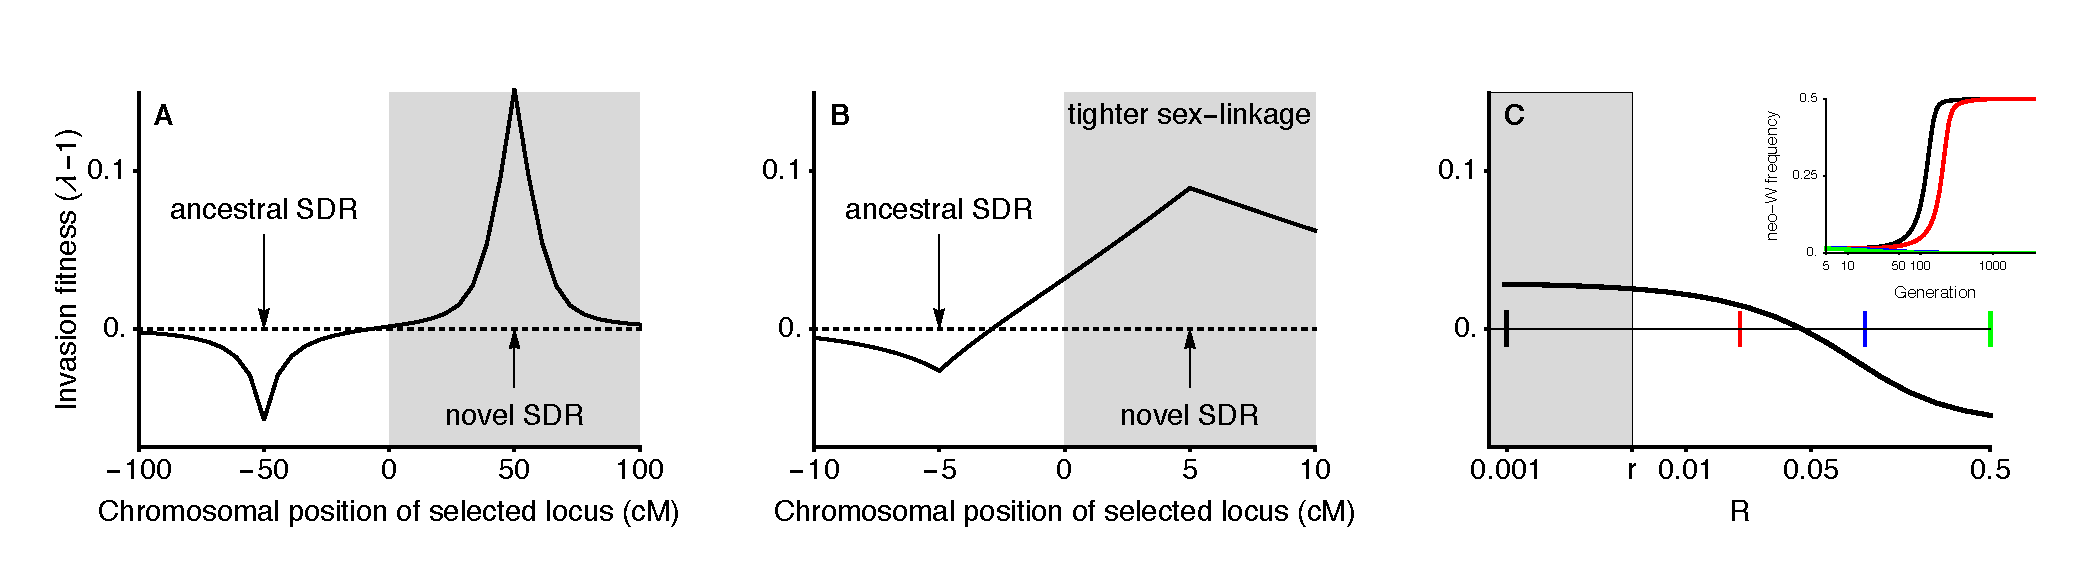
\includegraphics[width=1.5\linewidth]{PositionPlot_SexAntagTighter_Mike}}
\caption{
Transitions between XY and ZW systems can occur even when the neo-SDR is less tightly linked to a locus under sexually-antagonistic selection (here, without haploid selection).
In panel A, linkage is loose enough relative to selection that the analytical results assuming weak selection hold, and a neo-W can only invade when it is more tightly linked with the selected locus ($R<r$; shaded region).
In panel B, linkage is tight enough relative to selection that the analytical results assuming weak selection do not hold, and a neo-W can invade even when it is less tightly linked with the selected locus ($r<R$; unshaded region).
In panel C we vary the recombination rate between the neo-W and the selected locus ($R$) for a fixed recombination rate between the ancestral-SDR and the selected locus ($r=0.005$). 
Coloured markers show recombination rates for which the temporal dynamics of invasion are plotted in the inset, demonstrating that neo-W alleles can fix (reach frequency $0.5$ among female gametes) if they are more (black) or less (red) closely linked to a locus experiencing sexually-antagonistic selection. 
A very loosely linked neo-W does not spread in this case (blue and green lines overlap and go to 0). 
Indeed, we can show that neo-W invasion fitness is always negative when $R=1/2$ and there is sex-antagonism but no haploid selection (see supplementary \textit{Mathematica} file). 
Fitness parameters are shown by an asterisk in Figure \ref{fig:regionplots}A: $w_{AA}^\female = 1.05$, $w_{aa}^\male = 1.2$, $w_{aa}^\female = w_{AA}^\male = 0.85$, $w_{Aa}^\Hermaphrodite = 1$,  $t^\Hermaphrodite = \alpha^\Hermaphrodite_\Delta = 0$.
%\textcolor{red}{consider removing panel A, which is repeated in Figure 3.}
%\textcolor{blue}{probably better to remove from panel 3, eh?}
}
\label{fig:SexAntagTighter}
\end{figure}
%%%%%%%%%%%%%%%%%%%%%%%%%%%%%%%%%%%%%%%%%%%%%%%%%%%%%%%%%

If we categorise the $a$ allele as being ancestrally `male-beneficial' via the fact that it is fixed on the Y, then $\lambda_{mA}>1$ indicates that the neo-W spreads when found with the ancestrally `female-beneficial' allele. 
Broadly, this is possible because the ancestral X chromosome is sometimes found in males and is therefore unable to perfectly specialise on the `female-beneficial' allele. 
For example, when the $a$ allele is favoured in males, a polymorphism of $A$ and $a$ alleles can be maintained on the X despite directional selection in favour of the $A$ allele in females ($s^\female>0$, $0<h^\female<1$). 
When the $a$ allele is strongly favoured on X chromosomes in males ($w_{aa}$ sufficiently large relative to $w_{Aa}$), neo-W-$A$ haplotypes can spread ($\lambda_{mA}>1$), see Figure \ref{fig:regionplots}A.
In this case the $a$ allele is at high frequency among ancestral XX females due to selection upon the X in males. 
By contrast, W-$A$ haplotypes will only create females with high fitness ($AA$ or $Aa$ genotypes) and can therefore spread. 

When only one neo-W haplotype has a positive growth rate (see Figure \ref{fig:regionplots}), a neo-W can invade as long as equation \eqref{eq:lambdasGen} is satisfied, which may require that the recombination rate, $R$, is small enough.
Nevertheless, because we assume here that $r$ is small, these results indicate that a more loosely linked sex-determining region ($r<R$) can spread.
Therefore, tightly sex-linked loci that experience sexually-antagonistic selection can drive heterogametic transitions in which the neo-SDR is less closely linked to the locus under selection (Figure \ref{fig:SexAntagTighter}). 
%Prediction (just an idea), considering sexually antagonistic selection alone, we should observe an excess of transitions between XY and ZW systems on the same chromosome because the tight linkage results indicate that there can be selection for heterogametic transitions but only when the neo-SDR is relatively closely linked (but not necessarily more closely linked). 

Given that the $a$ allele can be considered ancestrally `male-beneficial' because it is fixed on the Y, it is surprising that neo-W-$a$ haplotypes can sometimes be favoured by selection in females ($\lambda_{ma}>1$). 
Again, this occurs because ancestral X's also experience selection in males, in which they will always be paired with a Y-$a$. 
Hence, if there is overdominance in males, X-$A$ Y-$a$ males have high fitness and the $A$ allele is favoured by selection on the X in males. 
Therefore, the X can be polymorphic or even fixed for the $A$ allele despite favouring the $a$ allele during selection in females \citep[e.g., see outlined region in Figure \ref{fig:regionplots}B and][]{Lloyd1977,Otto2014}. 
In such cases, neo-W-$a$ haplotypes can spread because they create more $Aa$ and $aa$ females when pairing with an X from males and because they bring Y-$a$ haplotypes into females. 

In some cases, both W-$A$ and W-$a$ haplotypes can spread, e.g., when $AA$ individuals have low fitness in females yet the $A$ is polymorphic or fixed on the X due to overdominance in males (Figure \ref{fig:regionplots}B and \ref{fig:regionplots}C).
Both neo-W-$A$ and neo-W-$a$ haplotypes then produce fewer unfit $AA$ females.
This is true for the neo-W-$A$ haplotype because it can pair with a Y-$a$ haplotype and still be female. 
Wherever both haplotypes have positive growth rates, invasion by a neo-W is expected regardless of its linkage with the selected locus (i.e., even unlinked neo-W alleles can invade, see Figures \ref{fig:positionOverdominance} and \ref{fig:temporalOverdominance} for examples). 

Assuming that linkage is not tight, \citet{vanDoorn:2010hu} showed that invasion by a neo-W occurs under the same conditions as `fixation' (where fixation indicates that the neo-W reaches its maximum frequency among eggs, which is 1/2). 
An equivalent analysis is not possible where we assume that linkage is tight. 
However, numerical simulations with tight linkage demonstrate that the neo-SDR does not necessarily fix, leading to the stable maintenance of a mixed sex-determining system, in which X, Y, Z, and W alleles all segregate (e.g., Figure \ref{fig:freqAll}B-D). 
Within a species, both feminizing and masculinizing alleles have been reported in houseflies \citep{Macdonald1978}, midges \citep{Thompson1971}, frogs \citep{Ogata:2007jm}, cichlid fish \citep{Ser:2010iq}, tilapia \citep{Lee2004}, sea bass \citep{Vandeputte2007}, and lab-strains of Zebrafish \citep{Liew2012,Wilson2014}. 
For example, in the platyfish (\textit{Xiphophorus maculatus}), X,Y, and W alleles segregate at one locus (or two closely-linked loci) near to potentially sexually-antagonistic genes for pigmentation and sexual maturity \citep{Kallman1965,Kallman1968, Volff2001, Schultheis2006}. 
Our results suggest that several forms of selection on nearby loci (i.e., $r$ and $R$ small) could maintain multiple sex-determining alleles. 

%Haploid selection impacts the spread of neo-W haplotypes through its direct selective effect on females and their gametes, its indirect effect on the marginal fitness of alleles in females resulting from haploid selection in male gametes, and its effect on the sex ratio.
%These impacts expand the scenarios under which neo-W haplotypes can spread.
%For instance, overdominance is no longer required for neo-W-$a$ haplotypes to spread when there is haploid selection (e.g., when $a$ is female-beneficial, $A$ is male-beneficial, and meiotic drive in males favours $a$, Figure \ref{fig:regionMaleDrive}B).
 


%%%%%%%%%%%%%%%%%%%%%%%%%%%%%%%%%%%%%%%%%%%%%%%%%%%%%%%%%
%Both neo-W haplotypes can spread, in the absence of haploid selection, when there is overdominance
%%%%%%%%%%%%%%%%%%%%%%%%%%%%%%%%%%%%%%%%%%%%%%%%%%%%%%%%%
\begin{figure}[!h]
\centering
\centerline{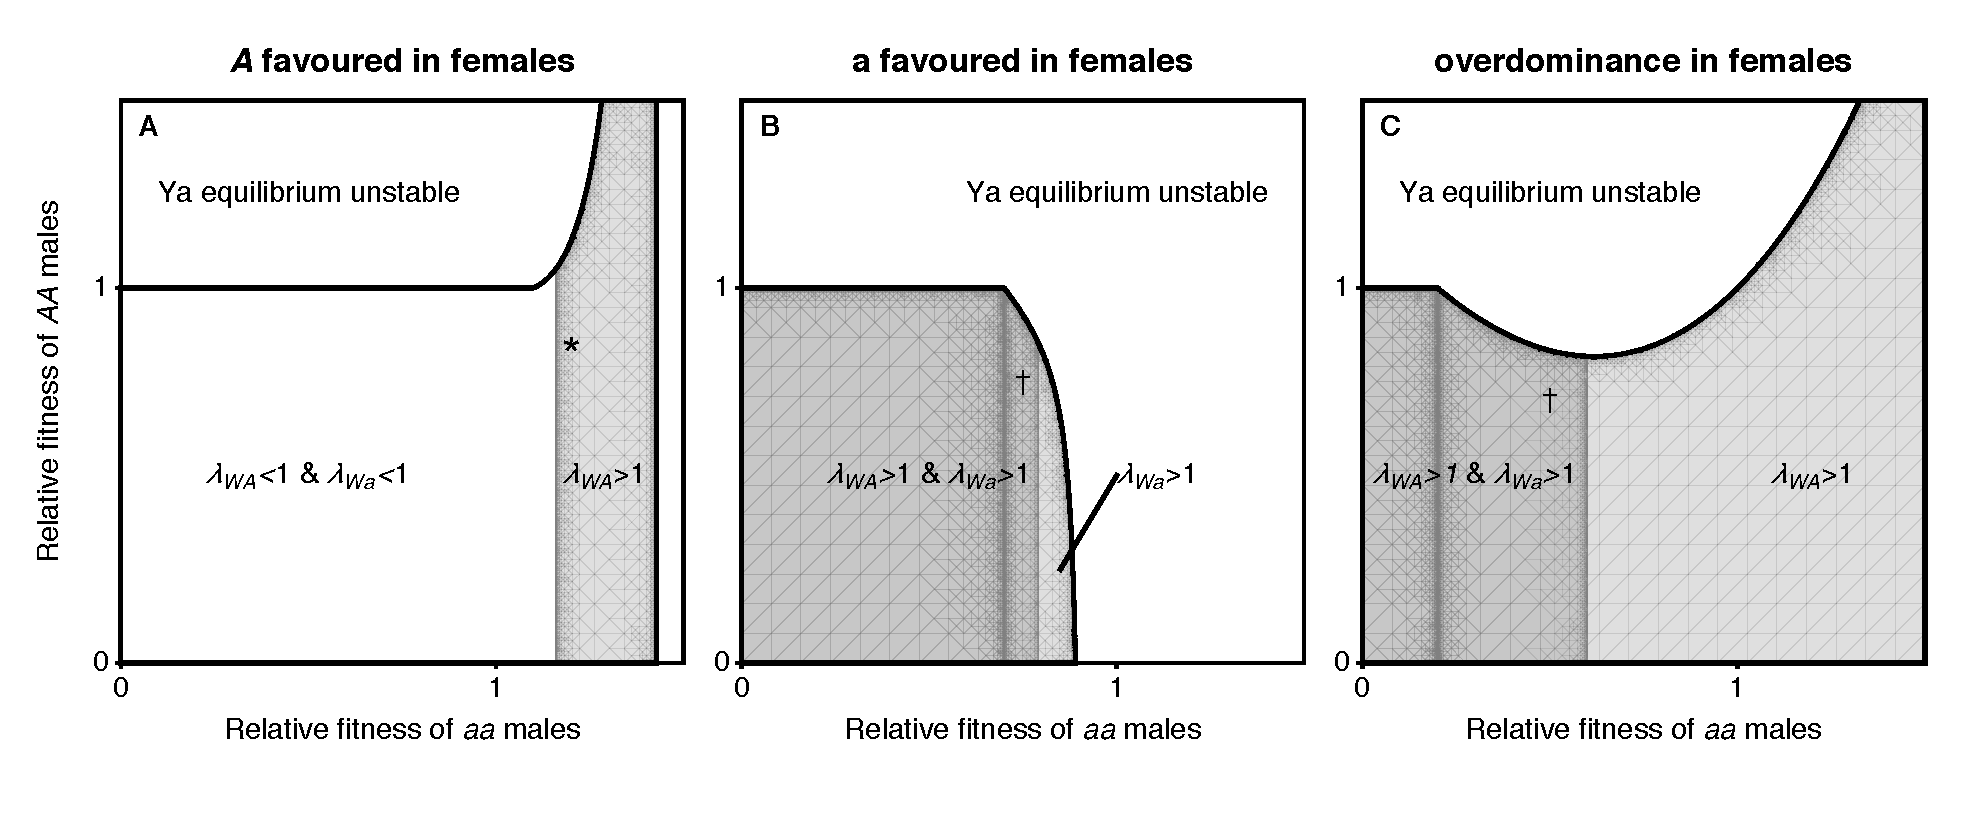
\includegraphics[width=1.25\linewidth]{Region_plot_combined_Mike}}
\caption{
When the ancestral-XY locus is tightly linked to a locus under selection ($r=0$), one or both neo-W haplotypes can spread. 
We vary the fitness of male homozygotes relative to heterozygotes ($w_{Aa}^\Hermaphrodite=1$) and only consider stable equilibria at which both \textbf{A} locus alleles are maintained and the $a$ allele is initially fixed on the Y, region outlined. 
Here, selection in females can favour the $A$ allele (panel A, $w_{aa}^\female=0.85$, $w_{AA}^\female=1.05$), favour the $a$ allele (panel B, $w_{aa}^\female=1.05$, $w_{AA}^\female=0.85$), or be overdominant (panel C, $w_{aa}^\female=w_{AA}^\female=0.6$). 
If $\lambda_{wA}$ or $\lambda_{wa}$ is greater than one, then a rare neo-W can spread for, at least, some values of $R>r$. 
For the parameter values marked with an asterisk, example invasion dynamics are shown in Figure \ref{fig:SexAntagTighter}C. 
Where both $\lambda_{wA}$ and $\lambda_{wa}$ are greater than one, a neo-W will spread when rare, regardless of linkage with the selected locus (for any $R$). 
Figure \ref{fig:positionOverdominance} shows two examples using the parameters marked with a dagger. 
Here, there is no haploid selection $t^\Hermaphrodite = \alpha^\Hermaphrodite_\Delta = 0$.
}
\label{fig:regionplots}
\end{figure}


%Neo-W alleles, on the other hand, can invade an ancestral XY system under some conditions (given in detail in the appendix). 
%%The full characteristic polynomials are given in the appendix (equations \ref{Binvasion} and \ref{Ainvasion}).
%Briefly, neo-W-$A$ and/or neo-W-$a$ haplotypes can spread when rare in the absence of recombination ($\lambda_{ma}>1$ and/or $\lambda_{mA}>1$), depending on the ancestral sex-ratio and allele frequencies. 
%Below we discuss the main forces determining the spread of these neo-W haplotypes and the impact of recombination for the overall success of the neo-W.
%To simplify our discussion we first outline the potential effects of haploid selection and then consider diploid selection in its absence.

%\textcolor{blue}{This explanation is clearer than the one I put in the appendix, if we drop it here, maybe we should try and re-word the corresponding part of the appendix using this paragraph}
%Haploid selection impacts the spread of neo-W haplotypes in three ways.
%Firstly, the zygotic sex ratio becomes male biased ($\zeta<1/2$) when the $a$ allele (which is fixed on the Y) is favoured during competition among male gametes or by meiotic drive in males. 
%This facilitates the spread of a neo-W because neo-W alleles cause the zygotes that carry them to develop as the rarer, female, sex. 
%Secondly, haploid selection in males affects the diploid genotypes of females by altering the allele frequencies in the male gametes that female gametes pair with.
%For instance, because an epistatically dominant neo-W always causes its carrier to become female, it creates females who carry either $Y-a$ or $X$ genotypes from their father.
%Thus, because when there is a polymorphism the $X$ carries some non-zero frequency of $A$, haploid selection in males impacts the diploid genotypes of females (e.g., creating more $Aa$ females when drive in males favours $Y-a$).
%How this affects the spread of the neo-W then depends on diploid and haploid selection in females.
%Thirdly, female drive and gamete competition directly select on neo-W haplotypes.
%Drive for $A$ in females favours neo-W-$A$ haplotypes, at a cost to neo-W-$a$ haplotypes, and vice-versa when there is drive for $a$.
%The impact of this drive depends on how often XX and neo-W females are heterozygous.
%Competition among female gametes acts similarly, and depends on the frequency of $A$ on resident X chromosomes (e.g., competition among eggs has no affect on the initial spread of the neo-W-$A$ haplotype when $A$ is fixed on the X).
%Because haploid selection in females favours one neo-W haplotype at the expense of the other, recombination off the favoured background becomes more detrimental as it becomes more favoured. Thus higher rates of recombination between the neo-W and the selected locus, $R$, can lead to smaller leading eigenvalues when there is haploid selection in females.

%In the absence of haploid selection and with the $A$ allele is fixed on the X, it is possible for both neo-W haplotypes can spread ($\lambda_{mA}>1$ and $\lambda_{ma}>1$ in \ref{Binvasion}), and thus neo-W invasion can occur regardless of its linkage to the selected locus.
%Invasion does not occur with purely sexually-antagonistic selection (i.e., $a$ directionally favoured in males and $A$ directionally favoured in females) because the X is then already as specialized as possible on the female sex.
%However, if, for example, $AA$ individuals suffer a fitness cost in females, yet $A$ is fixed on the X due to strong overdominance in males, both neo-W-$A$ and neo-W-$a$ haplotypes spread because they produce fewer unfit $AA$ females and never experience counter-selection in males.
%This is true even for the neo-W-$A$ haplotype because it can pair with a $Y-a$ haplotype and still be female. 
%When both haplotypes can spread alone the rate of recombination between the neo-W and the selected locus, $R$, does cannot prevent invasion, and thus the system can evolve looser sex-linkage (e.g., the neo-W could arise on an autosome, $R=1/2$).
%Even when only one haplotype can spread, invasion can still occur up to some positive rate of recombination, $R>0$ (as long as equation \ref{eq:lambdasGen} is satisfied). 
%That looser sex-linkage can evolve is contrary to the conclusions of \cite{vanDoorn:2010hu}, who did not explicitly calculate invasion fitness under ancestrally tight sex-linkage. \textcolor{blue}{or, just didn't calculate the equilibria (A) an (B).}
%Similar scenarios have been shown to select for a modifier that increases recombination between the sexes \citep[green regions of Figure 2 in][]{Otto2014}.
%\textcolor{blue}{n.b., the recombination regions are only subsets mostly because you also generate a really unfit Y haplotype through recombination. Probably not worth mentioning.}
%
%In the absence of haploid selection it is also possible for a neo-W to invade when there is a stable polymorphism at the $\mathbf{A}$ locus on X chromosomes.
%For example, overdominance in males and strong directional selection for $a$ in females creates a scenario that favours the spread of both neo-W haplotypes at equilibrium ($\lambda_{mA}>1$ and $\lambda_{ma}>1$ in \ref{Ainvasion}), as both haplotypes bring more $a$ alleles into females and never experience counter-selection in males.
%Thus, as in the case of the $A$ being fixed on the X, looser sex-linkage can evolve with a polymorphic X (i.e., $\lambda>1$ with $R>0$) and this is expected under the same scenarios that select for a modifier that increases recombination between the sex chromosomes \citep[blue regions of Figure 2 in][]{Otto2014}.

\subsubsection*{Loose linkage with the ancestral sex-determining region}


%\textcolor{blue}{As with the discussion, this section might need some editing for (1) unclearly describing looser linkage never evolving without haploid selection, which we now show is possible above and (2) going on about sex ratio selection too much - this should be changed to something along the lines of  ``male biased zygotic sex ratios ($\zeta-1/2$) are of the order of $\epsilon^2$. Therefore Fisherian sex ratio selection directly favours neo-Ws by a similar magnitude. 
%Perhaps surprisingly, neo-Ws can be favoured to the same degree by haploid selection in females when female haploid selection favours the alleles that tend to be carried by the neo-W.
%Thus XY to ZW is the same as ZW to XY even though sex ratio biases only exist in one case, given the assumptions made in this section.
%''
%}

%weak selection
%We are particularly concerned with whether or not a rare neo-sex-determining allele increases in frequency, which occurs when the largest eigenvalue, $\lambda$, is greater than one. 
%Here, we explicitly determine the conditions under which invasion occurs by assuming that the $A$ allele reaches an equilibrium frequency under the ancestral sex-determination system before the neo-sex-determination system ($m$) arises. 
%The equilibrium frequency of $A$ on different ancestral backgrounds ($\hat{p}^\male_Y$, $\hat{p}^\male_X$, and $\hat{p}^\female_X$) is given by equations \eqref{eq:pAve} and \eqref{eq:freq_diffs} where we assume selection and meiotic drive are weak relative to recombination ($s^\Hermaphrodite$, $t^\Hermaphrodite$, $\alpha_{\Delta}^\Hermaphrodite$ of order $\epsilon$). 
Assuming that selection is weak relative to all recombination rates ($r$, $R$ and $\rho$), we denote the leading eigenvalues describing the invasion of a neo-Y ($k=0$) and a neo-W ($k=1$) into an ancestrally XY system by $\lambda_{Y',XY}$ and $\lambda_{W',XY}$, respectively. To leading order in selection, these are:

\begin{equation}
\lambda_{Y',XY} =1+ V_{A}S_{A}^2\frac{ \left( r-R \right) }{r R}+O\left(\epsilon^3 \right) 
\label{eq:lambda_neoY}
\end{equation}

\noindent 
and 

\begin{equation}
\lambda_{W',XY} =\lambda_{Y',XY}+\left(2\alpha_{\Delta}^\male-2\alpha_{\Delta}^\female+t^\male-t^\female \right) \left( \hat{p}^\male_Y-\hat{p}^\male_X \right)/2
+O\left(\epsilon^3 \right) \\
\label{eq:lambda_neoW}
\end{equation}

\noindent
where $V_{A}=\bar{p}(1-\bar{p})$ is the variance in the equilibrium frequency of $A$ and $S_{A}=(D^\male +\alpha_{\Delta}^\male+t^\male) - (D^\female+\alpha_{\Delta}^\female+t^\female)$ describes sex differences in selection for the $A$ versus $a$ across diploid selection, meiosis, and gametic competition.
The diploid selection term, $D^\Hermaphrodite=\big{[} \bar{p}s^\Hermaphrodite+(1-\bar{p})h^\Hermaphrodite s^\Hermaphrodite\big{]} -\big{[} \bar{p}h^\Hermaphrodite s^\Hermaphrodite+(1-\bar{p}) \big{]}$, is the difference in fitness between $A$ and $a$ alleles in diploids of sex $\Hermaphrodite \in \{\female,\male\}$, where $\bar{p}$ is the leading-order probability of mating with an $A$-bearing gamete from the opposite sex (equation \ref{eq:pAve}). 
The difference in $A$-allele-frequency among Y-bearing sperm versus X-bearing sperm is given by $\hat{p}^\male_Y-\hat{p}^\male_X=V_{A}\big{(}D^\male - D^\female+\alpha_{\Delta}^\male-\alpha_{\Delta}^\female+t^\male-t^\female\big{)}(1-2r)/2r$. 


The neo-sex-determining allele, $m$, will spread if $\lambda_{m,XY}>1$. 
Equation \eqref{eq:lambda_neoY} demonstrates that, under weak selection, a neo-Y will invade an XY system if and only if it is more closely linked to the selected locus than the ancestral sex-determining region (i.e., if $R<r$; note that $V_{A}S_{A}^2$ is strictly positive as long as \textbf{A} is polymorphic). 
This echoes our tight linkage results above where a neo-Y could never invade if $r\approx0$. It is also consistent with the results of \citet{vanDoorn:2007eu}, who considered diploid selection only and also found that homogametic transitions (XY to XY or ZW to ZW) can only occur when the neo-sex-determining locus is more closely linked to a locus under sexually-antagonistic selection. 
%Because tighter linkage between the sex-determining region and a selected locus evolves during these transitions, stronger associations between selected alleles and diploid sexes can build up by selection (e.g., between male-beneficial alleles and the male-determining allele, Y).%, increasing diploid mean fitness (Figure \ref{fig:Combination_MeanFit}). 

With weak selection and no haploid selection ($t^\Hermaphrodite=\alpha^\Hermaphrodite_{\Delta}=0$), the spread of a neo-W is equivalent to the spread of a neo-Y ($\lambda_{W',XY}=\lambda_{Y',XY}$), such that heterogametic transitions (XY to ZW or ZW to XY) can also occur only if the neo-sex-determining region is more closely linked to a locus under selection ($R<r$), as found by \citet{vanDoorn:2010hu}. 
With haploid selection, however, the additional term in equation \eqref{eq:lambda_neoW} can be positive, which can allow, for example, neo-W invasion ($\lambda_{W',XY}>1$) even when the neo-sex-determining region is less closely linked to the selected locus ($R>r$). 
%These transitions are unusual because, when $R>r$, associations that selection has built up between alleles more favourable in one sex and alleles that determine sex will be weakened. 
%Mean diploid fitness therefore decreases during heterogametic transitions that create looser sex-linkage (Figure \ref{fig:Combination_MeanFit}B,D). 

%%%%%%%%%%%%%%%%%%%%%%%%%%%%%%%%%%%%%%%%%%%%%%%%%%%%%%%%%
%A neo-W can invade an XY system under a large number of selective regimes
%%%%%%%%%%%%%%%%%%%%%%%%%%%%%%%%%%%%%%%%%%%%%%%%%%%%%%%%%
\begin{figure}[!h]
\centering
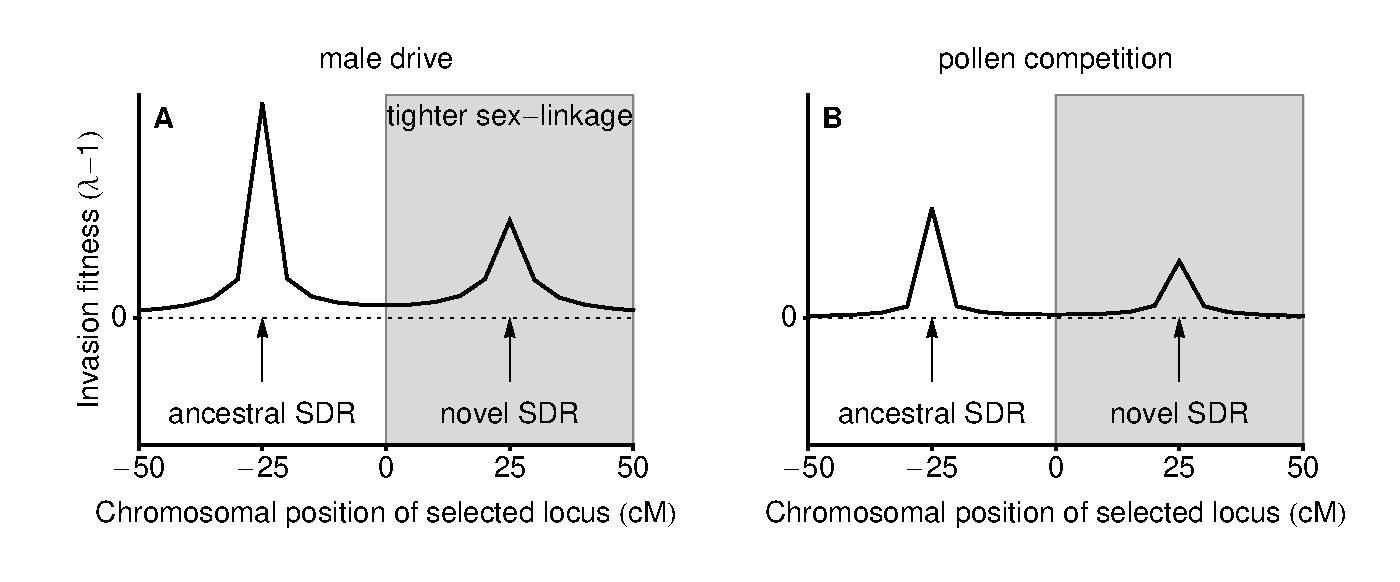
\includegraphics[width=\linewidth]{PositionPlot_8}
\caption{
% A neo-W can invade an XY system under a large number of selective regimes.
%In panel A, there is no haploid selection ($t^\Hermaphrodite = \alpha^\Hermaphrodite_{\Delta} = 0$) and selection in diploids is sexually antagonistic ($s^\male = -s^\female = 1/10$, $h^\male = 1-h^\female = 3/10$), in which case the neo-sex-determining allele can only invade if it is more closely linked to the selected locus ($R<r$, gray region; but see Figure \ref{fig:SexAntagTighter}B for the case of very tight linkage).
Ploidally-antagonistic selection allows a less tightly linked neo-W to invade.
In panel A, male drive ($\alpha^\male_{\Delta} = -1/20$, $t^\Hermaphrodite = \alpha^\female_{\Delta} = 0$) opposes selection in diploids (no sex-differences: $s^\Hermaphrodite = 1/10$, $h^\Hermaphrodite = 7/10$), in which case the neo-sex-determining allele can invade regardless of linkage.   
In panel B, gametic competition in males ($t^\male = -1/10$, $t^\female = \alpha^\Hermaphrodite_{\Delta} = 0$) opposes selection in diploids (sex-differences: $s^\male = 1/20$, $s^\female = 3/20$, $h^\Hermaphrodite = 7/10$), in which case the neo-sex-determining allele can once again invade regardless of linkage.
We use Haldane's map function \citep[Equation 3 in ][]{Haldane1919} to convert from map distance (centiMorgans, cM) to the probability of recombination (an odd number of cross-over events).   
%\textcolor{red}{Check the mismatch between red and black lines here: probably because of adding or subtracting from 1. }
%\textcolor{blue}{Can remove the mismatch by flipping the fitnesses between males and females (again). That is, if $M_{AA}$ is the fitness of $AA$ male diploids in an ancestral XY system, then $M_{AA}$ is the fitness of $AA$ female diploids in an ancestral ZW system. I think this makes sense in A, where we don't really want a difference between the red and black curves, but this makes less sense in B and C where we want to restrict haploid selection to males regardless of the ancestral system. We could just not flip the haploid fitnesses, but then does it make sense to flip the diploid fitnesses?}
}
\label{fig:Combination_Centimorgans}
\end{figure}
%%%%%%%%%%%%%%%%%%%%%%%%%%%%%%%%%%%%%%%%%%%%%%%%%%%%%%%%%


Equation \eqref{eq:lambda_neoW} shows that, with weak selection, neo-W alleles can invade an XY system for a large number of selective regimes. 
To clarify the parameter space under which $\lambda_{W',XY}>1$, we consider several special cases. 
Firstly, if the \textbf{A} locus is unlinked to the ancestral sex-determining region ($r=1/2$), a more closely linked neo-W ($R<1/2$) can always invade because there is no ancestral association between $A$ alleles and sex chromosomes in males, $\left( \hat{p}^\male_Y-\hat{p}^\male_X \right)=0$, see equation \eqref{eq:freq_diffs}. 
The second term in equation \eqref{eq:lambda_neoW} therefore disappears and invasion depends only on the sign of $(r-R)$. 
Indeed, invasion typically occurs when the neo-W is more closely linked to the selected locus than the ancestral sex-determining region (Figure \ref{fig:Combination_Centimorgans}).

Secondly, we can simplify the discussion of cases where invasion occurs despite looser sex-linkage, $R>r$, by focusing on the special case where $R=1/2$ and $r<1/2$ (e.g., the selected locus is on the ancestral sex chromosome and the novel sex-determining locus arises on an autosome). 
In Table \ref{tab:specialcases} we give the conditions where invasion occurs when we further assume that haploid selection only occurs in one sex (e.g., during male meiosis only) and dominance coefficients are equal in the two sexes, $h^\female=h^\male$. 
When there is no gametic competition and meiotic drive is in one sex only, an unlinked neo-W can invade as long as the same allele is favoured during diploid selection in males and females ($s^\female s^\male>0$, see Figure \ref{fig:Combination_Centimorgans}A and Figure \ref{fig:SexRatioBad}B). %, which is 50\% of the parameter space. 
When there is no meiotic drive and gametic competition occurs in one sex only, an unlinked neo-W can invade as long as the same allele is favoured in male and female diploid selection and there are sex differences in selection of one type (e.g., $s^\female(s^\male-s^\female)>0$, see Figure \ref{fig:Combination_Centimorgans}B). %, which is 25\% of the parameter space. 
These special cases indicate that neo-W invasion occurs for a relatively large fraction of the parameter space, even if the neo-W uncouples the sex-determining locus from a locus under selection. 

\begin{table}[ht]
\centering
\smallskip
\caption{Invasion conditions for unlinked neo-W ($R=1/2$, $r<1/2$) into ancestral XY with one form of haploid selection}
\begin{tabular}{l l c }
\hline\hline
Scenario &  Assumptions & neo-W spreads ($\lambda_{W',XY}>1$) if \\ [0.5ex] \hline
%  $r=1/2$, $R<1/2$ & Always \\ [0.5ex] \hline
%  $r<1/2$, $R=1/2$ &  \\ [0.5ex] \hline
\noalign{\vskip 1mm}
  male drive only & $h^\male=h^\female$, $t^\female=t^\male=\alpha^\female_{\Delta}=0$ & $s^\female s^\male>0$ \\ [0.5ex]
 female drive only & $h^\male=h^\female$, $t^\female=t^\male=\alpha^\male_{\Delta}=0$ & $s^\female s^\male>0$ \\ [0.5ex]
 sperm competition only &  $h^\male=h^\female$, $t^\female=\alpha^\female_{\Delta}=\alpha^\male_{\Delta}=0$ & $s^\female(s^\male-s^\female)>0$ \\ [0.5ex]
  egg competition only & $h^\male=h^\female$, $t^\male=\alpha^\female_{\Delta}=\alpha^\male_{\Delta}=0$ & $s^\male(s^\female-s^\male)>0$ \\ [0.5ex]
  \hline \hline
  \label{tab:specialcases}
 \end{tabular}
\end{table}


%If we further assume equal dominance ($h^\female=h^\male$) and that haploid selection only occurs during male meiosis ($t^\female=t^\male=\alpha^\female_{\Delta}=0$), or female meiosis ($t^\female=t^\male=\alpha^\male_{\Delta}=0$), neo-W invasion occurs when $s^\female s^\male>0$, Figure \ref{fig:Combination_Centimorgans}B.
%That is, when the same allele is favoured by selection in both males and females (it may remain polymorphic via counter selection during meiotic drive). 

%\textcolor{red}{It may seem counterintuitive that, if the $A$ allele is more common on the ancestral-Y than the ancestral-X, and only favoured during haploid selection in males}

%\textcolor{red}{although our predictions also perform well when recombination is small, see figure \ref{fig:WinvasionLowR}. We would have to add a line showing what invasion fitness the weak selection approximation would give and add dots to this figure (dots that are currently connected by a line), as in (vD\&K, 2010) }

%Sex ratios
%Previous research suggests that when the ancestral sex-determining locus is linked to a locus that experiences haploid selection (e.g., meiotic drive), a new, unlinked sex-determining locus invades in order to restore equal sex ratios \citep{Kozielska:2010vm}. 
%Our model provides a good opportunity to determine whether Fisherian sex-ratio selection provides a useful explanation for the evolution of new sex-determining loci in other contexts. 
%Consider, for example, the case where the \textbf{A} locus is linked to the ancestral-SDR ($r<1/2$) and experiences meiotic drive in males only (e.g., during spermatogenesis but not during oogenesis, $\alpha^\male \neq 1/2$, $\alpha^\female=1/2$). 
%We will also disregard gametic competition ($t^\female=t^\male=0$) such that zygotic sex ratios are only biased by meiotic drive in males. 
%In this case, the zygotic sex ratio can be initially biased only if the ancestral sex-determining system is XY (Figure \ref{fig:Combination_Turnover}B). 
%If the ancestral sex-determining system is ZW, the zygotic sex ratio will be 1:1 because diploid sex is determined by the proportion of Z-bearing versus W-bearing eggs and meiosis in females is fair (Figure \ref{fig:Combination_Turnover}D).
%Thus, if the zygotic sex ratio is crucial to the evolution of new genetic sex-determining systems, invasion into ZW and XY systems will be distinct. 
%However, under weak selection we find that invasion by a homogametic neo-sex-determining allele (XY to XY or ZW to ZW) or by a heterogametic neo-sex-determining allele (XY to ZW or ZW to XY) occur under the same conditions. 
%That is, we can show that $\lambda_{Y',XY}=\lambda_{W',ZW}$ and $\lambda_{Y',ZW}=\lambda_{W',XY}$ (at least up to order $\epsilon^3$; for a numerical example, compare Figure \ref{fig:Combination_Turnover}A,B to Figure \ref{fig:Combination_Turnover}C,D).
%As it turns out, under weak selection the strength of sex-ratio selection favouring, say, the invasion of a neo-W in an XY system is the same as the strength of meiotic drive favouring the invasion of a neo-Y in a ZW system. 
%Even when these forces are not exactly the same (e.g., under tight sex-linkage; compare black and red curves near -25 and 25cM in Figure \ref{fig:Combination_Centimorgans}), it is important to remember that sex-ratio selection is only one of many potential selective forces acting to determine transitions between sex-determining systems.
%It is even possible for the other selective forces to overwhelm sex-ratio selection and favour sex-determination transitions that create sex-ratio biases (Figure \ref{fig:Combination_Turnover}A,C).

Previous research suggests that when the ancestral sex-determining locus is linked to a locus that experiences haploid selection (e.g., meiotic drive), a new, unlinked sex-determining locus invades in order to restore equal sex ratios \citep{Kozielska:2010vm}. 
Consider, for example, the case where the \textbf{A} locus is linked to the ancestral-SDR ($r<1/2$) and experiences meiotic drive in males only (e.g., during spermatogenesis but not during oogenesis, $\alpha^\male_\Delta \neq 0$, $\alpha^\female_\Delta=0$), without gametic competition ($t^\female=t^\male=0$).
In this case, the zygotic sex ratio can be initially biased only if the ancestral sex-determining system is XY (Figure \ref{fig:SexRatioBad}B). 
%If the ancxestral sex-determining system is ZW, the zygotic sex ratio will be 1:1 because diploid sex is determined by the proportion of Z-bearing versus W-bearing eggs and meiosis in females is fair (Figure \ref{fig:Combination_Turnover}D).
We might therefore expect a difference in the potential for XY to ZW and ZW to XY transitions. 
However, to leading order with selection weak relative to recombination, we find that sex ratio selection favours the spread of a neo-W (through the first terms in table \ref{tab:haplotype_growth}) by an amount that is equal in magnitude to the fitness effects of alleles associated with new sex-determining alleles (second terms in table \ref{tab:haplotype_growth}).
Thus, invasion by a neo-W into an XY system and invasion by a neo-Y into a ZW system occur under the same conditions ($\lambda_{Y',XY}=\lambda_{W',ZW}$ and $\lambda_{Y',ZW}=\lambda_{W',XY}$, at least to order $\epsilon^2$).
For example, in Figure \ref{fig:SexRatioBad}B neo-W alleles invade an ancestrally-XY system where females are initially rare because the ancestral-Y is associated with a male meiotic drive allele.
However, Figure \ref{fig:SexRatioBad}A shows that a neo-Y can invade an ancestrally-ZW system under the same conditions. 
In fact, where $R<1/2$ the neo-Y becomes associated with the male meiotic drive allele such that the zygotic sex ratio evolves to become biased towards males.

%As selection becomes stronger (or linkage becomes tighter), this symmetry between sex-ratio selection and haploid selection is lost, causing differences in the strength of selection favouring the two heterogametic transitions (compare red to black near -25cM and 25 cM in Figure \ref{fig:Combination_Centimorgans}). \textcolor{red}{normalise fitness in sexually antagonistic case}

%%%%%%%%%%%%%%%%%%%%%%%%%%%%%%%%%%%%%%%%%%%%%%%%%%%%%%%%%
%Sex-ratio selection is not a good predictor of neo-W invasion into an XY system
%%%%%%%%%%%%%%%%%%%%%%%%%%%%%%%%%%%%%%%%%%%%%%%%%%%%%%%%%
\begin{figure}[!h]
\centering
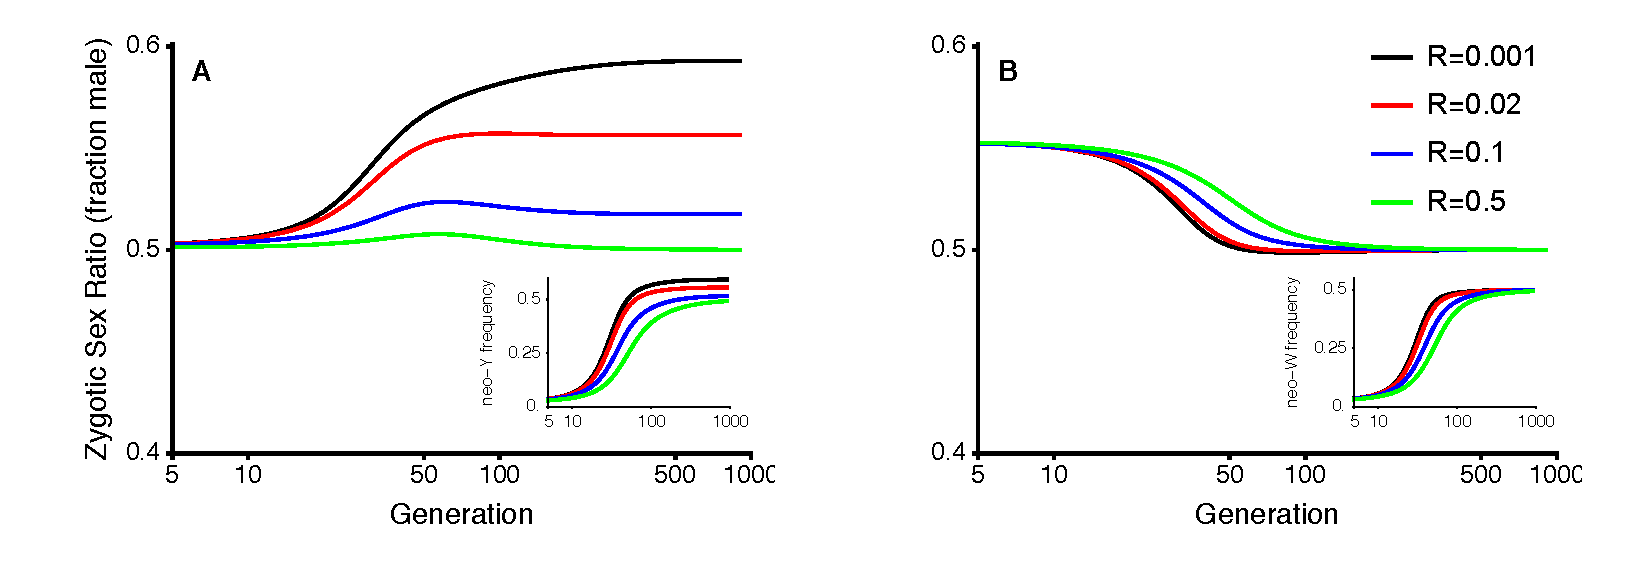
\includegraphics[width=\linewidth]{Temporal_SR_Mike}
\caption{
Fisherian sex-ratio selection alone is not a good predictor of turnover between sex-determining systems.
In this figure, selection is ploidally antagonistic with haploid selection favouring the $a$ allele during male meiosis.
In panel A, male drive in an ancestral ZW system has no affect on the zygotic sex ratio, yet a neo-Y can invade and replace the ancestral sex-determination system (inset shows neo-Y frequency among male gametes, the ancestral W also goes to fixation during this transition). 
When $R<1/2$, the neo-Y becomes associated with the allele favoured by drive, causing the zygotic sex ratio to become biased, hence the frequency of neo-Y among male gametes can be higher than $0.5$ (inset).
In panel B, male drive in an ancestral XY system causes a male bias, allowing a neo-W to invade and replace the ancestral sex-determination system (inset shows neo-W frequency among female gametes, the ancestral Y also goes to fixation), which balances the zygotic sex ratio.
Parameters:  $s^\female =s^\male = 0.2$, $h^\female = h^\male = 0.7$, $t^\female = t^\male = \alpha^\female_\Delta = 0$, $\alpha^\male_\Delta = -0.1$, $r=0.02$.
}
\label{fig:SexRatioBad}
\end{figure}
%%%%%%%%%%%%%%%%%%%%%%%%%%%%%%%%%%%%%%%%%%%%%%%%%%%%%%%%%

The green curves in Figure \ref{fig:SexRatioBad} shows transitions between male and female heterogametey even though the new sex-determining region is unlinked to a locus that experiences haploid and diploid selection. 
We use these green curves to discuss why heterogametic transitions can occur when $R=1/2$ and $r<1/2$, as in Table \ref{tab:specialcases}.
In Figure \ref{fig:SexRatioBad}B, an unlinked neo-W can spread because the zygotic sex ratio is ancestrally male biased. 
In Figure \ref{fig:SexRatioBad}A, an unlinked neo-Y spreads despite the fact that the ancestral zygotic sex ratio is even. 
In this case, the the male meiotic drive allele, $a$, is initially more common among ancestral-Z-bearing eggs than ancestral-W-bearing eggs because the Z is found in males more often than the W ($\hat{p}_{W}^\female-\hat{p}_{Z}^\female>0$, equation \ref{eq:freq_diffs}). 
%In this case, the ancestral male determining allele, Z, is initially associated with the male meiotic drive allele, $a$, because the Z is found in males more often than the W and $r<1/2$. 
Polymorphism at the \textbf{A} locus is maintained by counter-selection against the $a$ allele in diploids and therefore ancestral-ZZ males have generally low diploid fitness. 
The neo-Y spreads because it produces males with high diploid fitness through matings with ancestral-W-bearing female gametes, which are more likely to carry the $A$ allele. 
A freely recombining neo-Y ($R=1/2$) is equally likely to be segregate with the $A$ or $a$ allele and is therefore unaffected by male meiotic drive.
Thus, a key factor in explaining why heterogametic transitions can occur when $R>r$ is that that the neo-SDR determines sex in the diploid phase but recombination occurs before any subsequent haploid selection. 

%Therefore Fisherian sex ratio selection directly favours neo-Ws by a similar magnitude. 
%Perhaps surprisingly, neo-Ws can be favoured to the same degree by haploid selection in females when female haploid selection favours the alleles that tend to be carried by the neo-W.
%Thus XY to ZW is the same as ZW to XY even though sex ratio biases only exist in one case, given the assumptions made in this section

\subsubsection*{Environmental sex determination}

We next consider the case where the new sex-determining mutation, $m$, causes sex to be determined probabilistically or by heterogeneous environmental conditions (environmental sex determination, ESD), with individuals carrying allele $m$ developing as females with probability $k$.
Here, we do not assume that the environmental conditions that determine sex also differentially affect the fitness of males versus females. 
Such correlations can favour environmental sex-determination systems that allow each sex to be produced in the environment in which it has highest fitness; in the absence of these correlations, previous theory would predict that ESD is favoured when it produces more equal sex ratios than the ancestral system \citep[see reviews by][]{Charnov:1982wg,Bull:1983vi,West:2009we}. %(e.g., maternal condition, mate quality, age, or host size)  

The characteristic polynomial determining the eigenvalues (equations \ref{eq:recursions}) does not factor for ESD mutants as it does for $k=0$ or $k=1$. 
We therefore focus on weak selection here. 
Assuming weak selection, the spread of the new sex-determining region is given by 

\begin{equation}
\begin{split}
\lambda_{ESD',XY} =& 1 + (1-2k)^2V_{A}{S_{A}}^2\frac{r-R}{r R} \\
&+\frac{k(\hat{p}^\male_Y-\hat{p}^\male_X)}{2}\left[ k \left(2\alpha_{\Delta}^\male-2\alpha_{\Delta}^\female+t^\male-t^\female \right) -4(1-k)S_{A}\right]+O\left(\epsilon^3\right),
\end{split}
\label{eq:lambda_ESD_k}
\end{equation}

\noindent
which reduces to $\lambda_{Y',XY}$ when $k=0$ and $\lambda_{W',XY}$ when $k=1$. 

%Under Fisherian sex-ratio selection, autosomal modifiers favour equal investment in male and female offspring, i.e., a 1:1 sex ratio \citep{Fisher:1930wy,Charnov:1982wg,West:2009we}. 
%A novel environmental sex-determiner that causes half of its carriers to become female and half to become male ($k=1/2$) will be in males half of the time and in females half of the time (like an autosome).
%In addition, these novel sex-determination alleles equalize the sex ratio and therefore one might expect them to be favoured by Fisherian sex-ratio selection when the resident sex ratio is biased.
%However, assuming weak selection, we find that the growth rate of a rare, dominant offspring-controlled neo-ESD allele that produces males or females with equal probability ($k=1/2$) is
Of particular interest are ESD mutations that cause half of their carriers to develop as females and half as males ($k=1/2$, creating equal sex ratios), the spread of which is given by
\begin{equation}
\lambda_{ESD',XY} =1+ \frac{1}{2}\frac{(\lambda_{Y',XY\rvert R=1/2}-1) + (\lambda_{W',XY\rvert R=1/2}-1)}{2} + O\left(\epsilon^3\right),
%V_A \frac{r}{1-2r}  \frac{s_{f} \left( s^\male - 3 s^\female\right) }{8 \left( s_{f} + s_{m} \right)^2} t_{m}^2.
\label{eq:lambda_ESD}
\end{equation}
\noindent
where $\lambda_{Y',XY\rvert R=1/2}$ and $\lambda_{W',XY\rvert R=1/2}$ represent $\lambda_{Y',XY}$ and $\lambda_{W',XY}$ when evaluated at $R=1/2$ (Equations \ref{eq:lambda_neoY} and \ref{eq:lambda_neoW}).
That is, recombination between the selected locus and the novel sex-determining locus, $R$, doesn't enter into the $k=1/2$ results.
This is because sex is essentially randomized each generation, %as if the novel sex-determiner were on an unlinked site that half the time acts as a neo-$W$ and half the time as a neo-$Y$.
preventing associations from building up between allele $A$ and sex. 
Equation \eqref{eq:lambda_ESD} shows that the neo-ESD gets half of the fitness of a feminizing mutation (neo-$W$) and half of the fitness of a masculinizing mutation (neo-$Y$), but only has an effect one half of the time (the other half of the time it produces the same sex as the ancestral system would have, to leading order). 
As discussed above, $\lambda_{Y',XY\rvert R=1/2}$ is necessarily less than one, but $\lambda_{W',XY\rvert R=1/2}$ can be greater than one if there is haploid selection.
That is, when there is haploid selection, ESD mutations can invade an ancestrally-XY system because they generate females that are either rare or have high fitness, in the same manner as a neo-W. 

%An important result from equation \eqref{eq:lambda_ESD} is that ESD can invade if there is haploid selection. 
%When evaluated at $R=1/2$, $\lambda_{Y',XY}$ is necessarily less than one, but $\lambda_{W',XY}$ can be greater than one if there is haploid selection, as discussed above. 
%Previous studies where ESD is favoured have typically assumed that environmental conditions (e.g., maternal condition, mate quality, age, or host size) can differentially affect the fitness of males versus females such that ESD invades because it allows sex determination to depend on the environment \citep[reviewed in][]{Charnov:1982wg,Bull:1983vi,West:2009we}. 
%Here, ESD mutations can spread because they generate females that are either rare or have high fitness, in the same manner as a neo-W. 

Significantly, equation \eqref{eq:lambda_ESD} is the same whether ESD is invading an ancestrally XY or ZW system (because $\lambda_{Y',XY} = \lambda_{W',ZW}$ and $\lambda_{W',XY} = \lambda_{Y',ZW}$).
Thus, Fisherian sex-ratio selection alone does not explain the invasion of ESD under weak selection because the sex ratio is only biased by male haploid selection when the ancestral sex-determination system is XY. 
Specifically, with male haploid selection, the neo-ESD is equally likely to invade when it equalizes the zygotic sex ratio (through $\lambda_{W',XY}$) and when it doesn't (through $\lambda_{Y',ZW}$). 
%This is again because haploid selection can facilitate the turnover of sex chromosomes either through sex ratio biases or through associations between the new sex determining region with selected alleles. 
%With weak selection, these two forces are nearly equal in strength. 
In addition, we note that ESD may not invade, even if the sex ratio is initially biased (e.g., with drive in males only, $r<1/2$, $h^\female=h^\male$, and $s^\female s^\male<0$, such that $\lambda_{W',XY}<1$, see Table \ref{tab:specialcases}). 


%Depends 50\% on its fitness relative to non-mutant males and 50\% on its fitness relative to non-mutant females. 

%\subsubsection*{Maternally-controlled neo-ESD}

%Fisherian sex-ratio selection is sometimes considered in terms of balancing parental investment in male versus female offspring \citep{Charnov:1982wg}.
%In addition, under environmental sex-determination, the proportion of males/females is sometimes controlled by the mother (e.g., the proportion of eggs laid in warm versus cold environments). 
%We therefore also considered the invasion of a neo-sex-determining allele ($m$) in a model in which mothers that have at least one $m$ allele produce daughters with probability $k$. 
%As with offspring-controlled ESD, for all $k\in\{0,1/2,1\}$, we find that invasion into an ancestral XY system is the same as invasion into an ancestrally ZW system (at least up to order $\epsilon^3$, assuming weak selection), implying that transitions between genetic sex-determination and maternally controlled environmental sex-determination are not driven by Fisherian sex-ratio selection alone.
%\textcolor{red}{(Maternal ESD analysis still lacks meiotic drive -- Mathematica can't seem to deal with the added complexity.)}

%One might think that when the sex of zygotes is under the control of mothers, there would be strong selection to balance the sex ratio among zygotes. 
%However, we find that, with no meiotic drive and weak selection, the invasion fitness of a dominant, maternally controlled sex-determiner that produces proportion $k$ daughters can be written
%\begin{equation}
%\lambda_{k} = 1 + V_A S_A C_k + O\left(\epsilon^3\right),
%\end{equation}
%where
%\begin{equation}
%V_A = \frac{- \left[ t_m + h (s_{f}+s_{m}) \right] \left[ t_m + (1-h) (s_{f}+s_{m}) \right]}{(1-2h)^2(s_{f}+s_{m})^2}
%\end{equation}
%is the variance in $A$ ($V_A>0$ when the polymorphic resident equilibrium is stable), 
%with $h$ the dominance coefficient (equal in both sexes), 
%$C_k$ is a term that depends on $k$.
%
%%k=0
%\begin{equation}
%C_0 = big \; ugly \; term
%\end{equation}
%
%%k=1
%\begin{equation}
%C_1 = \frac{\left[ (2r(1-R)-R) s^\female + (1-2r)R s^\male \right]}{2}
%\end{equation}
%
%%k=1/2
%\begin{equation}
%C_{1/2} = even \; bigger, \; uglier \; term
%\end{equation}
%
%When $k=1$ the maternal- and offspring-controlled results are the same, $C_1 = C_W$, since the mutation remains in females (and hence mutant daughters always have mutant mothers).
%However, with $k\neq1$ the results with maternal control differ from those with offspring control.
%Interestingly, for all $k\in\{0,1/2,1\}$, we find that invasion into an ancestrally XY system is the same as invasion into an ancestrally ZW system (at least up to order $\epsilon^3$), implying that sex-ratio selection does not drive transitions between genetic sex determination and maternally controlled environmental sex determination.
%Of particular interest is $k=1/2$ (i.e., when the mother perfectly balances the sex ratio of her offspring).
%When both recombination rates are small we have $C_{1/2} \approx R(s^\male - s^\female)/8 = \lim_{r \rightarrow 0} C_1/4$.
%This implies that, at least under tight linkage, the invasion of maternally-controlled ESD is independent of $R$ (because $S_A\propto R^{-1}$) and can invade whenever a neo-$W$ can (which can invade even when it biases the sex ratio further; Figures \ref{fig:WinvasionLowR} -- \ref{fig:WinvasionHighR}).


\section*{Discussion}

%\textcolor{blue}{maybe re-order to put the results up front and focus on sex ratio less. Somewhere around these first two paragraphs we should include our tight linkage results. At the moment it doesn't make total sense because it assumes that tighter linkage is always favoured unless there is haploid selection.}


%MAIN RESULT
Two predominant theories explaining the remarkably high frequency of transitions between sex-determination systems are sexually-antagonistic selection and sex-ratio selection \citep[reviewed in][]{Blaser2012, vanDoorn2014re}.
The former predicts that neo-sex-determining alleles can invade when they arise in closer linkage with a sexually-antagonistic locus \citep{vanDoorn:2007eu,vanDoorn:2010hu}.
The latter predicts that new sex-determining systems are generally favoured if they result in more equal sex-ratios than the ancestral system. 
%The latter predicts that neo-W alleles will invade an XY system when there is a male bias caused by haploid selection in males, and vice-versa, a neo-Y will invade a ZW system when there is a female bias caused by haploid selection in females \citep{Kozielska:2010vm,Ubeda:2015fx}.
Firstly, we show that selection (including sexually-antagonistic selection) on loci within or near the non-recombining region of the ancestral sex-determining region can favour heterogametic transitions (XY to ZW or ZW to XY) to new sex-determining systems that are less closely linked to the selected loci (e.g., see Figure \ref{fig:SexAntagTighter}). 
Secondly, assuming that selection is weak relative to recombination (`weak selection'), we show that new sex-determining alleles are typically favoured if they are more closely linked to a locus under haploid selection, which is the only condition favouring homogametic transitions (XY to XY or ZW to ZW). 
In addition, with haploid selection and weak selection, heterogametic transitions (XY to ZW or ZW to XY) can occur even when the new sex-determining region is less closely linked to the locus under selection (e.g., see Figure \ref{fig:SexRatioBad}). 
%\textcolor{red}{need to mention sex ratio here}
%Neo-W (neo-Y) alleles invade when their fitness in females (males) is greater than the mean fitness of females (males) under the ancestral sex-determination system and/or females (males) are the rarer sex.


%TIGHT LINKAGE RESULTS
%When the rate of recombination between the ancestral sex-determining locus and a locus under selection is small relative to the strength of selection (i.e., sex-linkage is tight, or selection is strong), heterogametic transitions (XY to ZW or ZW to XY) that reduce sex-linkage are possible, with or without haploid selection (Figures \ref{fig:SexAntagTighter} and \ref{fig:regionplots}).

%The likelihoods of these transitions are driven by sex-ratio selection, direct selection on alleles linked to the neo-sex-determining allele, the ability of the neo-sex-determining allele to avoid selection in one sex, and the ability of the neo-sex-determining allele to bring alleles on the sex-specific chromosome in the ancestor into the other sex (given that the neo-sex determining allele is epistatically dominant to its predecessor).

%This possibility that looser sex-linkage could evolve, even in the absence of haploid selection (Figure \ref{fig:regionplot_2a}A), was overlooked in \cite{vanDoorn:2010hu}, likely because they did not explicitly consider the case of initially tight linkage between the \textbf{A} locus and the ancestral-SDR, which allows substantial differences in allele frequencies to build up \citep[$\hat{p}^\Hermaphrodite_{X} \neq \hat{p}_{Y}^\male$, equation \ref{eq:tightequil};][]{Lloyd1977,Otto2014}.
%Interestingly, there is substantial overlap between the parameter space that allows both neo-W-$A$ and neo-W-$a$ haplotypes to spread in an XY system and that which selects for increased recombination between X and Y chromosomes \citep[e.g., compare gray region of Figure \ref{fig:regionplot_2a}A with coloured regions of Figure 2(a) in][]{Otto2014}.
%This makes sense, as when both neo-W haplotypes can spread the neo-W can invade despite reducing sex-linkage, i.e., the rate of recombination between the sex-determining allele and the selected locus increases.
%We further find that it is easier for a neo-W to invade 
%\textcolor{red}{explain difference too? also explain why a neo-Y doesn't invade to reduce linkage despite selection for more recombination? mention something about haploid selection (Fig7B)?} \textcolor{blue}{maybe leave for now}


%HAPLOID SELECTION CAN ACT LIKE SEXUALLY-ANTAGONISTIC SELECTION
%It has previously been demonstrated that new sex-determining systems can evolve if there is genetic variation maintained by sexually-antagonistic selection \citep{vanDoorn:2007eu,vanDoorn:2010hu}. 
%In particular, 
%Under weak selection (or loose sex-linkage), transitions to new sex-determining systems can occur when they arise more closely linked to a sexually-antagonistic locus \citep{vanDoorn:2007eu,vanDoorn:2010hu}.
%New sex-determining alleles are again favoured if they are more closely linked to a locus under haploid selection, which is the only condition favouring homogametic transitions (XY to XY or ZW to ZW).
%HAPLOID SELECTION ALSO ALLOWS LOOSER LINKAGE TO EVOLVE
%However, with haploid selection, heterogametic transitions (XY to ZW or ZW to XY) can occur even when the new sex-determining region is less closely linked to the locus under selection. 
%Neo-W (neo-Y) alleles invade when their fitness in females (males) is greater than the mean fitness of females (males) under the ancestral sex-determination system and/or females (males) are the rarer sex.

%With sexually-antagonistic selection (between diploid sexes) only, linkage between a selected locus and the sex-determining region strengthens associations between male beneficial alleles and the male-determining allele (Y or Z) and between female beneficial alleles and the female-determining allele (X or W). 
%Thus, the mean fitness of both males and females increases with closer linkage to the sex-determining region. 
%Therefore, new sex-determining alleles only invade if they are more closely linked than the ancestral sex-determining region. 
%However, if there is haploid selection on loci linked to an XY (ZW) sex-determining region, selection can maintain polymorphisms at which the product of the frequency of females (males) and the mean fitness of females (males) is lower than it would be without sex-linkage. 
%In these cases, unlinked neo-W (neo-Y) alleles can increase the frequency and/or fitness of the only sex they are found in, at a cost to the other sex, and invade despite lowering population mean fitness (Figure \ref{fig:Combination_MeanFit}). 
%\textcolor{red}{This is similar to mitochondria and male disease ...?}

%%SEX-RATIO SELECTION
%\textcolor{blue}{maybe drop paragraph?}
%\textcolor{red}{I messed with the sex-ratio selection paragraphs to tone down our "it doesn't matter" speech from before. Have at any amendments you'd like to make.}
%Linkage between haploid selected loci and sex-determining regions cases biased zygotic sex ratios \citep{Hamilton:1967ts,Burt:2006,Field:2012fd,Field:2013cc}.
%One might then expect Fisherian sex-ratio selection to drive the spread of new sex-determining systems that bring the sex ratio closer to 50:50. 
%Fisherian sex-ratio selection follows from the fact that, for an autosomal locus, half of the genetic material is inherited from a male, and half from a female \citep{Fisher:1930wy,West:2009we}. 
%Thus, if the population sex ratio is biased towards females, the average per-individual contribution of genetic material to the next generation from males is greater than the contribution from females (and vice versa for male-biased sex ratios). 
%Therefore, a mutant that increases investment in males will spread via the higher per-individual contributions made by males. 
%%%That is, under Fisherian sex-ratio selection, the success of a mutant relative to the non-mutant depends, in equal parts, on the contributions made by males and females to the next generation. 
%An implicit assumption of Fisherian sex-ratio selection is that the mutant allele is autosomal and has the same inheritance pattern as the non-mutant allele. 
%The mutations we consider here, neo-sex-determining alleles, break this assumption. 
%For example, the success of neo-Y/neo-W mutations depends only on the number of alleles contributed by males/females (Table \ref{tab:haplotype_growth}). 
%In this respect, a neo-W is similar to a cytoplasmic element, which also does not experience selection to balance sex ratios \citep{Frank:1989vl,Werren:1998co,Chase:2007bf}.
%Even mutants that are equally likely to be found in males or females, such as an environmental sex determination mutation (equation \ref{eq:lambda_ESD}), are not strictly autosomal if they determine sex. 
%Thus, despite the fact that sex ratio biases caused by gametic competition or meiotic drive have been shown to exert Fisherian sex-ratio selection on various autosomal modifiers \citep{Stalker:1961th,Smith:1975ft,Frank:1989vl,Hough:2013uo,Ubeda:2015fx, Otto:2015va}, we do not find evidence of Fisherian sex-ratio selection acting during invasion by neo-sex-determination systems (e.g., see Figure \ref{fig:Combination_Turnover} and \citealt{Ubeda:2015fx}, in which a neo-Y invades despite biasing sex ratios). 

%Sex ratio biases caused by gametic competition or meiotic drive have been shown to exert Fisherian sex-ratio selection on various autosomal \citep{Stalker:1961th,Smith:1975ft,Frank:1989vl,Hough:2013uo,Ubeda:2015fx, Otto:2015va} and sex-linked \citep{Kozielska:2010vm} modifiers.
Sex-ratio biases caused by haploid selection can facilitate heterogametic transitions between sex-determining systems. 
For instance, alleles favoured by haploid selection in males often become associated with the Y, which leads to a male-biased zygotic sex-ratio.
This male bias increases the potential for a neo-W to invade (Table \ref{tab:haplotype_growth}), which can equalize the sex-ratio \citep[e.g., see Figure \ref{fig:SexRatioBad}B, for related examples see][]{Kozielska:2010vm,Ubeda:2015fx}.
%We find that sex-ratio biases caused by haploid selection can also affect transitions between sex-determining systems (e.g., see $\zeta$ terms in Table \ref{tab:haplotype_growth}). 
%However, the neo-W may not equalize the sex-ratio (e.g., if the driving allele also drives in females or affects competition among eggs)
However, sex-ratio selection can be overwhelmed by additional selective effects (e.g., when a linked allele is beneficial for male diploids but detrimental for female diploids; Table \ref{tab:specialcases}), preventing the neo-W from invading. %and equalizing the sex ratio.
Indeed, transitions between sex-determining systems can even lead to stronger sex-ratio biases.
For example, where a neo-Y invades and is linked with a locus that experiences haploid selection in male gametes, the sex ratio evolves to become biased \citep[e.g., see Figure \ref{fig:SexRatioBad}A and step 1 in][]{Ubeda:2015fx}.
%For example, in an ancestral ZW system, haploid selection in males can allow a linked neo-Y to invade, despite the fact that it creates a male-biased sex ratio because the neo-Y becomes associated with the driven allele (Figure \ref{fig:SexRatioBad}A).
%\textcolor{blue}{and figure 1, where the end of one panel is the same as the beginning of another, however, this figure may change).}
%What we would like to stress is that sex-ratio selection alone cannot predict when new sex-determining systems can evolve.
Furthermore, with weak selection, we find that there is no difference in conditions allowing XY to ZW and ZW to XY transitions, indicating that sex chromosome transitions are not predominantly predicted by their effect on the sex-ratio (i.e., the sex-ratio bias created by male haploid selection facilitates the spread of a neo-W into an XY system the same way that male haploid selection drives the spread of a neo-Y into a ZW system with a 1:1 sex ratio). 
%An asymmetry can develop when sex-linkage is tight (e.g., Figure \ref{fig:Combination_Centimorgans} near -25cM and 25cM) but under most circumstances we do not predict asymmetry between XY to ZW and ZW to XY transitions despite the presence/absence of sex ratio selection. 
Thus, haploid selection can favour heterogametic transitions both via sex-ratio selection %\citep[as predicted by][]{Kozielska:2010vm} 
and via fitness effects of alleles that are associated with the neo-sex-determining allele, and these selection pressures are predicted to often be of equal magnitude when selection is weak. 
%\textcolor{red}{Maybe try to emphasise surprisingness in the paragraph more? e.g., how wrong you'd be if you assumed selection to equalise sex ratios, or it this implied?}
%\textcolor{blue}{nice, pretty subtle argument but I think that's a good job.}

%Previous studies where ESD is favoured have typically assumed that environmental conditions (e.g., maternal condition, mate quality, age, or host size) can differentially affect the fitness of males versus females such that ESD invades because it allows sex determination to depend on the environment \citep[reviewed in][]{Charnov:1982wg,Bull:1983vi,West:2009we}. 

%SEX-RATIO BIAS IN UBEDA ET AL
%DRAFT (improve): In \citet{Ubeda:2015fx}, the new sex determining locus spreads because it arises in linkage with a locus that experiences drive. They assume that drive occurs predominantly in one sex, e.g., during spermatogenesis or a 'killer' sperm. A driving allele is maintained at an intermediate frequency by selection, e.g., because it causes male sterility when homozygous (because all male sperm are killed). Y chromosomes that arise in linkage with the driving allele spread because they allow drive to occur more often, thus genetic sex determination with a sex ratio bias evolves. 
%Thus \citet{Ubeda:2015fx} also find that genetic sex determiners can invade, despite causing sex ratios to become biased. 
%Finally, they show that autosomal 'restorers' that negate the effects of meiotic drive can invade and restore an equal sex ratio. 

%WHY SEX-RATIO BIASES CAN BE FAVOURED
%We note two other ways in which sex determination has been shown to relate to zygotic sex ratios.
%Firstly, female-biased sex ratios can be favoured when there is local mate competition, where all matings are between siblings and assuming one male can inseminate many females \citep{Hamilton:1967ts}. 
%Therefore, with local mate competition, feminizing mutations can spread because they bias the sex ratio towards females \citep{Wilson:1981vm,Vuillleumier:2007bh}. 
%Secondly, environmental conditions (e.g., maternal condition, mate quality, age, or host size) can differentially affect the fitness of males versus females such that the optimal allocation to males/females depends on the environment \citep{Trivers:1973wb,Charnov:1977tx,Charnov:1982wg}. 
%In such cases, flexible sex-determination systems may evolve in order to allow the zygotic sex ratio to be determined in a way that depends on the environment \citep{Charnov:1977tx,Werren:1984tl,Pen:2010kk}. 
%In this study, we do not consider environmental condition dependence or local mate competition \citep[reviewed in][]{Charnov:1982wg,Bull:1983vi,West:2009we}. 

%HOW TO TEST EMPIRICALLY
%\textcolor{blue}{I think Sally was sceptical of this idea. i.e., if the second term in \ref{eq:lambda_neoW} is negative, then get less transitions with haploid selection included, right? }
%\textcolor{red}{Yeah, and given that only 1/2 the discovered plant sex chromosomes are hetermorphic and there are so few plant sex chromosomes to begin with (Charlesworth 2016 Annual Review Plant Biology), might it be the case that haploid selection is constraining things? perhaps we could think of some particular forms of haploid selection that might be common and give their predicted effects, or just say some things that are possible with haploid selection that are not without it -- if there are any. just looking at eq 3 though, its gonna be hard to get a low freq of A on the Y if haploid selection in males favours A, i.e., it should often be positive when there is no female haploid selection, right?}
%\textcolor{blue}{That sounds right to me and is backed up by equation \eqref{eq:freq_diffs}. It may be technically possible for that term to be negative though. Re: hetermorphism, I see that as a slightly different issue. It's thought that haploid selection may prevent deletions from becoming fixed on the Y, like in the Crowson (2017) paper. 
%I think the issue of `why so few plant sex chromosomes' is partly an issue of detection and also `why so much hermaphroditism'. Is it possible that the ESD results could show selective forces that also favour transitions from dioecy to hermaphroditism? I think so. Our ESD mutant produces 1/2 females and 1/2 males whereas a hermaphrodite invests roughly equally in each type of gamete produced. We don't consider the forces that are usually thought to be involved in these transitions though (inbreeding depression, reproductive assurance and possibly others?). }
%Taken at face value, our results indicate that transitions in heterogametey (XY to ZW or vice versa) are more likely to be favoured by selection if there is selection upon both haploid and diploid genotypes rather than diploid selection alone (). 
%This prediction could be examined using a suitable proxy for haploid selection, for example, \cite{Lenormand:2005vb} use the outcrossing rate in plants as a proxy for the strength of pollen competition. 
%In animals, one might expect gametic competition to be stronger in species where sperm is required to live for a long time after spermatogenesis because transcripts shared during spermatogenesis may become depleted, revealing the haploid phenotype of the sperm \citep{Immler:2014im}. 
%Given the caveats mentioned above about the form of meiotic drive modelled, we would also expect that heterogametic transitions in sex determination would be more common in clades where there is meiotic drive.

%Together, our models demonstrate novel selective forces that favour heterogametic transitions (XY to ZW or ZW to XY). 
%One common prediction is therefore that heterogametic transitions are favoured under a wider range of conditions than homogametic transitions. 
%However, heterogametic transitions are not clearly in excess. For example, \citet{Vicoso:2015hf} found a dozen sex chromosome configurations among Dipteran species but only one transition between male and female heterogametey. 
%While our models examine the selective forces that favour the spread of new sex-determining regions, observed transitions could also reflect the mutation rate for neo-Y versus neo-W alleles (e.g., duplications of the ancestral sex determining region could be particularly likely). 
%In addition, heterogametic transitions could be limited due to the production of YY males or WW females (see below). 
%Alternatively, it might be useful to compare clades that are expected to differ in the strength of haploid selection (e.g., plants are thought to experience more selection during their multicellular haploid stage

%COMPARATIVE PATTERNS 
We have shown that the spread of new sex determination systems can be driven by loci experiencing haploid selection. 
Because haploid selection can cause transitions that increase or decrease sex-linkage, haploid selection may lead to less stability, and greater potential for cycling, in sex-determination systems (e.g., the final state of the red line in Figure \ref{fig:SexRatioBad}A is the starting state in Figure \ref{fig:SexRatioBad}B). 
In particular, if haploid selection is strong but selective differences between male and female diploids are weak, we find that heterogametic transitions (XY to ZW or vice versa) are favoured more strongly than homogametic transitions (e.g., with $|D^\male - D^\female| << |\alpha_\Delta^\male - \alpha_\Delta^\female + t^\male - t^\female|$ we have $\lambda_{W',XY} > \lambda_{Y',XY}$; Equations \ref{eq:lambda_neoW} and \ref{eq:freq_diffs}). 
Turnovers driven by haploid selection may help to explain the relative rarity of heteromorphic sex chromosomes in plants, which are thought to experience more selection during their multicellular haploid stage.
For example, among relatively few dioecious clades in which multiple species have well characterized sex chromosomes \citep{Ming:2011iy}, heterogametic transitions have been inferred in \textit{Silene} subsection \textit{Otites} \citep{Slancarova:2013dq} and in \textit{Salicaceae} \citep{Pucholt2015,Pucholt2017}.
%Potentially, successive heterogametic transitions between master regulators of sex-determination could be inferred from careful examination of the molecular pathways by which sex is determined. 
%Our predictions could also be examined using a suitable proxy for haploid selection, for example, \cite{Lenormand:2005vb} use the outcrossing rate in plants as a proxy for the strength of pollen competition. 
Furthermore, assuming that transitions from dioecy to hermaphroditism (equal parental investment in male and female gametes) are favoured in a similar manner to the ESD examined here (equal probability of zygotes developing as males or females), our results suggest that competition during the haploid stage could drive transitions between dioecy and hermaphroditism, which are frequent in plants \citep{Kafer2017, Goldberg2017}.
%In animals, one might expect gametic competition to be stronger in species where sperm is required to live for a long time after spermatogenesis because transcripts shared during spermatogenesis may become depleted, revealing the haploid phenotype of the sperm \citep{Immler:2014im}.
%We would also expect that heterogametic transitions in sex determination would be more common in clades where there is meiotic drive. 

%IDENTIFICATION OF LOCI IN GENOMIC LOCATIONS THAT IMPLICATE THEM IN SEX-CHROMOSOME TURNOVER
%The hypotheses presented here can be empirically investigated in a similar manner to the idea that transitions between sex-determining systems are favoured by linkage to sexually-antagonistic variation. 
%In the case of sexually-antagonistic variation, one supporting observation is that genes expected to be under sexually-antagonistic selection (e.g., those causing bright male colouration) have been found on recently derived sex chromosomes \citep{Lindholm:2002dw,Tripathi:2009cw,Ser:2010iq}. 
In support of their role in sex chromosome turnover, genes expected to be under sexually-antagonistic selection (e.g., those causing bright male colouration) have been found on recently derived sex chromosomes \citep{Lindholm:2002dw,Tripathi:2009cw,Ser:2010iq}. 
Our results show that, if loci experiencing overdominance and/or sexually-antagonistic selection can be identified in close linkage with the ancestral sex-determining locus (rather than only the novel sex-determining locus), then they could also be implicated in driving heterogametic transitions between sex-determination systems. 
%As noted by \citet{vanDoorn:2010hu}, it would be prudent to compare closely related clades in order to determine whether observed polymorphisms predate a transition in sex-determination or arose afterwards. %, particularly because sex-linkage allows sexually-antagonistic selection to maintain polymorphisms under a different and larger parameter space \citep{Rice:1987hs,Jordan:2011fj}. 
 In addition, we show haploid selection on loci around either the ancestral- or the novel-sex-determining regions could have had a role in driving sex chromosome turnover. 
%Our results suggest that polymorphic loci that are ancestrally sex-linked and under sex-specific selection could also drive heterogametic transitions between sex-determination systems. 
%As with sexually-antagonistic selection, the presence of haploid selected loci around ancestral- or novel-sex-determining regions could support their role in sex chromosome turnover.
%We note that linkage with sex chromosomes is not, a priori, more permissive to the maintenance of ploidally antagonistic variation \citep{Immler:2012tl}. 
A recent transcriptome analysis in \textit{Rumex}, suggests a role for gametic competition in the evolution of sex-determination systems, showing that Y-linked genes are have higher expression in haploid pollen than autosomal genes \textcolor{red}{(check this is accurate)}.
Interestingly, haploid-expression is also more common on the autosome that is orthologous to the sex chromosomes in closely related species suggesting that new sex chromosomes may have been favoured through their association with haploid selected alleles on these chromosomes \textcolor{red}{(Sandler et al., 2017, Personal Communication)}.

%Limitation 1: DEGENERATE Y
We assume that sex-determining alleles do not experience direct selection except via their associations with sex and selected alleles.
However, in some cases, there may be significant degeneration around the sex-limited allele (Y or W) in the ancestral sex-determining region because recessive deleterious mutations and/or deletions accumulate around the Y or W sex-determining regions \citep{Rice:1996ke,Charlesworth:2000cc,Bachtrog:2006ed,Marais:2008hm}. 
During heterogametic transitions (XY to ZW or ZW to XY), but not homogametic transitions (XY to XY or ZW to ZW), any recessive deleterious alleles linked to the Y or W are revealed to selection in YY or WW individuals \citep{Bachtrog:2014bx}. 
This phenomenon was studied by \citet{vanDoorn:2010hu}, who found that degeneration can prevent fixation of a neo-W or a neo-Y allele, leading to a mixed sex-determination system where the ancestral and new sex-determining loci are both segregating. 
However, they noted that very rare recombination events around the ancestral sex-determining region can allow these heterogametic transitions to complete.  
%While not explicitly studied, we also predict that Y or W degeneration would prevent fixation of the new sex-determining genes considered here.
Degeneration around the Y or W could explain why heterogametic transitions are not observed to be much more common than homogametic transitions despite the fact that our models demonstrate that they are favoured under a wider range of conditions. 
For example, \citet{Vicoso:2015hf} found a dozen sex chromosome configurations among Dipteran species but only one transition between male and female heterogametey. 

%Limitation 2: TWO ALLELE DRIVE
Another simplification that we made is that meiotic drive involves only a single locus with two alleles. 
However, many meiotic drive systems involve an interaction with another locus at which alleles may `suppress' the action of meiotic drive \citep[][]{Burt:2006,Lindholm:2016cw}.
Thus, the dynamics of meiotic drive alleles can be heavily dependent on the interaction between two loci and the recombination rate between them, which in turn can be affected by sex-linkage if there is reduced recombination between sex chromosomes \citep{Hurst:1991uh}.
Furthermore, in some cases, a driving allele may act by killing any gametes that carry a `target' allele at another locus, in which case there can be fertility effects which can affect the equilibrium frequency of a meiotic drive allele \citep{Holman:2015en}. 
In polygamous mating systems, the intensity of pollen/sperm competition can depend on the density of males available to donate pollen/sperm, which can itself depend on the sex ratio \citep{Taylor:2002wu}. 
In terms of our model, this implies that the strength of gametic competition ($t^\male$) may both determine and be determined by the sex ratio. 
How the evolution of new sex-determining mechanisms could be influenced by two-locus meiotic drive and/or by ecological feedbacks under different mating systems remains to be studied.

%\textcolor{blue}{similarly, this part doesn't discuss our new tight linkage results or our new perspective on sex ratios.}
%CONCLUSION
We have shown that tight sex-linkage and haploid selection can drive previously unexpected transitions between sex-determination systems.
In particular, both can select for neo-sex-determining loci that are more loosely linked. 
In addition, haploid selection alone can cause transitions analogous to those caused by purely sexually-antagonistic selection, eliminating the need for differences in selection between male and female diploids.
Perhaps counterintuitively, transitions involving haploid selection can be driven by sex-ratio selection or cause sex-ratio biases to evolve. 
We conclude that haploid selection should be considered as a pivotal factor driving transitions between sex-determination systems. 
Overall, our results suggest several new scenarios under which new sex-determination systems are favoured, which could help to explain why the evolution of sex-determination systems is so dynamic. 
%Further, we have shown the way in which transitions are affected by haploid selection is not intuitively obvious. 
%Firstly, sex-specific haploid selection affects turnovers between sex-determination systems in a manner that is qualitatively different from diploid sex-specific selection. 
%In particular, closer linkage between a sex-determining locus and a selected locus is not always favoured during heterogametic transitions when there is haploid selection. 
%Secondly, even though haploid selection is a source of zygotic sex-ratio biases, in our models Fisherian sex-ratio selection does not have good explanatory power in determining whether various sex-determination systems evolve. 
%This result is surprising given that sex ratios are ultimately determined via the sex-determination system, and leads us to the conclusion that three selective forces -- haploid, diploid, and sex-ratio selection -- should all be considered when exploring transitions between sex-determination systems.


\bibliographystyle{amnatnat.bst}
\bibliography{sex_chromosomes.bib}

\newpage
%\section*{Figures}
%\newpage

%%%%%%%%%%%%%%%%%%%%%%%%%%%%%%%%%%%%%%%%%%%%%%%%%%%%%%%%%
%Tighter linkage allows looser sex-linkage to evolve, even in absence of haploid selection
%%%%%%%%%%%%%%%%%%%%%%%%%%%%%%%%%%%%%%%%%%%%%%%%%%%%%%%%%
%\begin{figure}[!h]
%\centering
%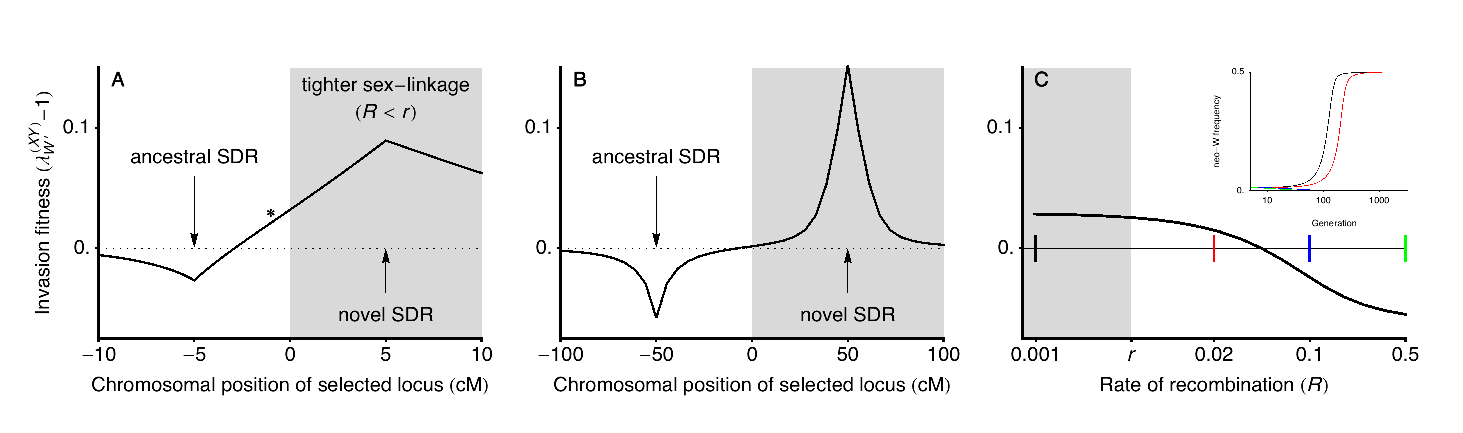
\includegraphics[width=\linewidth]{PositionPlot_SexAntagTighter}
%\caption{
%In the absence of haploid selection, tight linkage allows looser sex-linkage to evolve in transitions between XY and ZW systems.
%In panel A, linkage is loose enough relative to selection that the weak selection analytical results hold, and a neo-W can only invade when it is more tightly linked with the selected locus ($R<r$; shaded region).
%In panel B, linkage is tight enough relative to selection that the weak selection analytical results do no hold, and a neo-W can only invade even when it is less tightly linked with the selected locus ($r<R$; unshaded region).
%Parameters: $w_{AA}^\female = w_{aa}^\male = 1.05$, $w_{aa}^\female = w_{AA}^\male = 0.85$, $w_{Aa}^\female = 1$, $w_{Aa}^\male = 0.925$, $t^\Hermaphrodite = \alpha^\Hermaphrodite_\Delta = 0$.
%}
%\label{fig:SexAntagTighter}
%\end{figure}
%%%%%%%%%%%%%%%%%%%%%%%%%%%%%%%%%%%%%%%%%%%%%%%%%%%%%%%%%
%\newpage

%%%%%%%%%%%%%%%%%%%%%%%%%%%%%%%%%%%%%%%%%%%%%%%%%%%%%%%%%
%Both neo-W haplotypes can spread, in the absence of haploid selection, when there is overdominance
%%%%%%%%%%%%%%%%%%%%%%%%%%%%%%%%%%%%%%%%%%%%%%%%%%%%%%%%%
%\begin{figure}[!h]
%\centering
%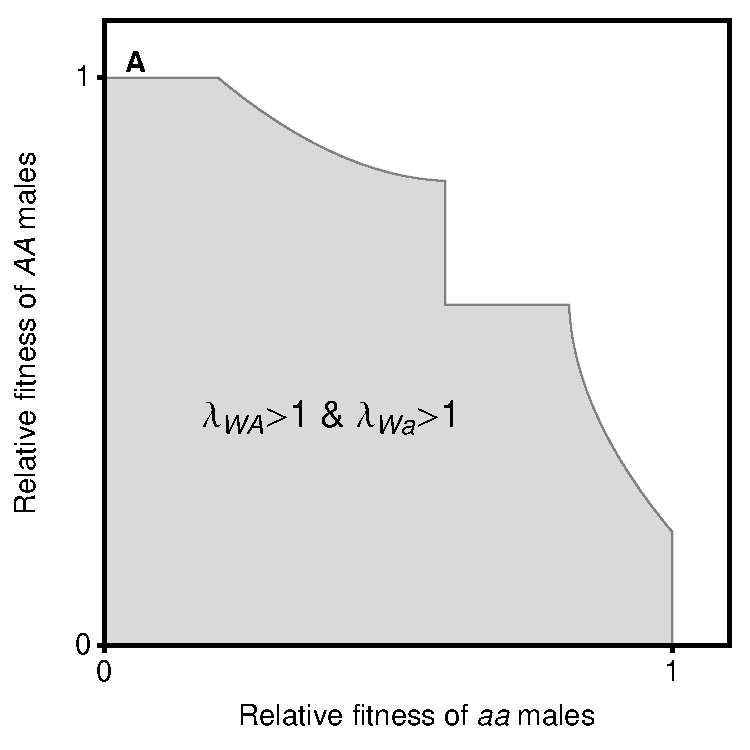
\includegraphics[width=0.45\linewidth]{regionplot_2a}
%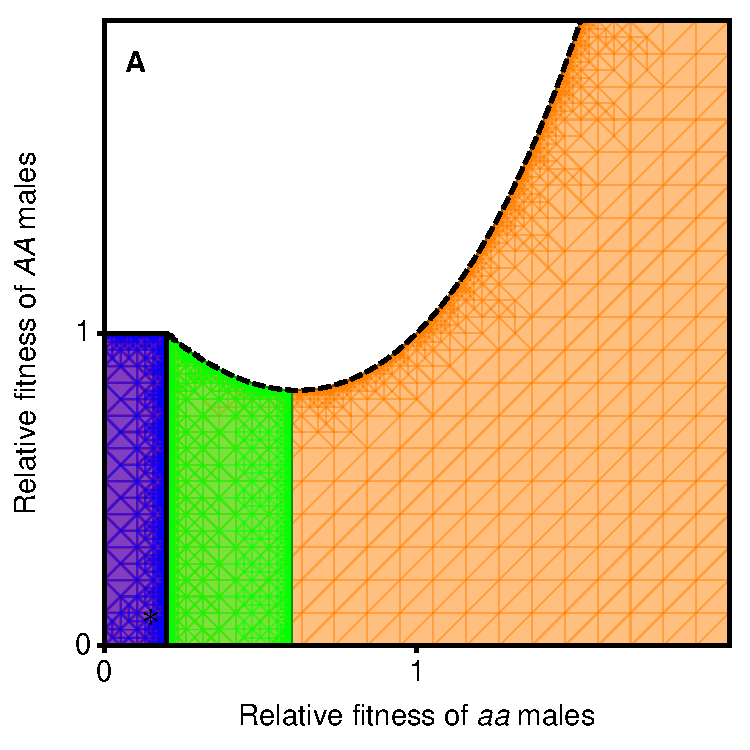
\includegraphics[width=0.45\linewidth]{regionplot_2a_Color_Ya_Either}
%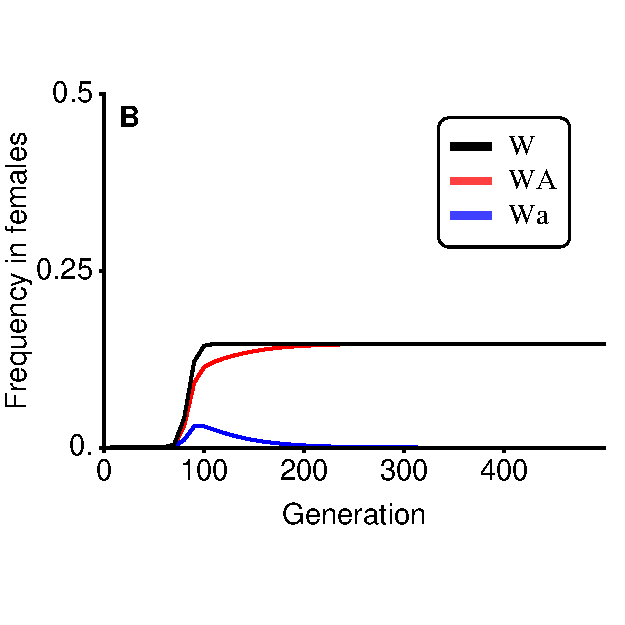
\includegraphics[width=0.45\linewidth]{BothWsInvade_Overdominance}
%\caption{
%In the absence of haploid selection, both neo-W haplotypes can spread in an XY system when there is overdominance.
%Panel A shows the range of male homozygote fitnesses that allow either neo-W haplotypes to invade.
%The blue region overlaps with a red region, where both neo-W haplotypes can invade a population with $A$ fixed on the X and $a$ fixed on the Y.
%The green region (overlapped by the orange region) is where both neo-W haplotypes can invade a population with $a$ fixed on the Y and a polymorphic X.
%The orange region (outside the green region) is where only the neo-W-$A$ haplotype can invade
%Panel B shows the temporal dynamics of the invading neo-W haplotypes; in this case the neo-W does not fix, leading to a polymorphic sex-determining system.
%Asterisk in panel A marks parameter values ($w_{aa}^\male=0.15$, $w_{AA}^\male=0.1$) used in panel B.
%Parameters: $w_{AA}^\female = w_{aa}^\female = 0.6$, $w_{Aa}^\Hermaphrodite = 1$, $t^\Hermaphrodite = \alpha^\Hermaphrodite_\Delta = 0$, $r=R=0$.
%\textcolor{red}{make two more temporal plots with visible asterisks in green and orange regions; figure out better colours to show possibilities}
%}
%\label{fig:BothOverdominance}
%\end{figure}
%%%%%%%%%%%%%%%%%%%%%%%%%%%%%%%%%%%%%%%%%%%%%%%%%%%%%%%%%
%\newpage

%%%%%%%%%%%%%%%%%%%%%%%%%%%%%%%%%%%%%%%%%%%%%%%%%%%%%%%%%
%With weak selection, a less tightly linked neo-W can invade an XY system when there is some haploid selection, and this invasion decreases mean diploid fitness
%%%%%%%%%%%%%%%%%%%%%%%%%%%%%%%%%%%%%%%%%%%%%%%%%%%%%%%%%
%\begin{figure}[!h]
%\centering
%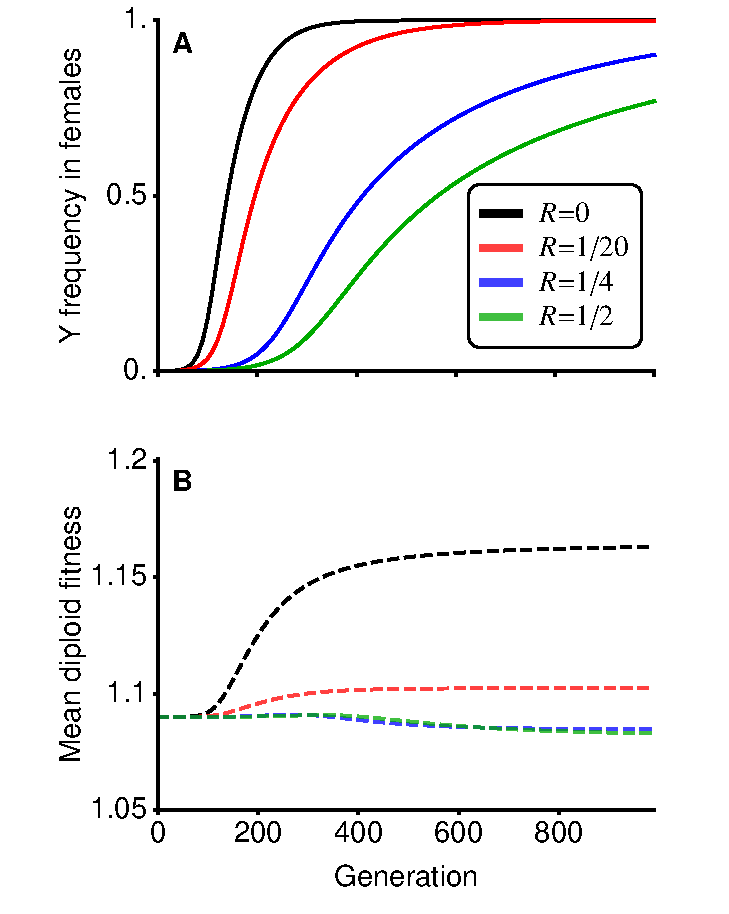
\includegraphics[width=0.5\linewidth]{Loose_Fitness_Decline}
%\caption{
%With weak selection, a less tightly linked neo-W can invade (and fix in) an XY system (causing the Y to fix in females) when there is some haploid selection (blue and green curves in panel A), and this invasion decreases mean diploid fitness (green and blue curves in panel B).
%Parameters: $s^\Hermaphrodite = 0.2$, $h^\Hermaphrodite = 0.7$, $t^\Hermaphrodite = \alpha^\male_\Delta = 0$, $\alpha^\female_\Delta = -0.1$, $r=1/10$.
%}
%\label{fig:LooseDecline}
%\end{figure}
%%%%%%%%%%%%%%%%%%%%%%%%%%%%%%%%%%%%%%%%%%%%%%%%%%%%%%%%%
%\newpage

%%%%%%%%%%%%%%%%%%%%%%%%%%%%%%%%%%%%%%%%%%%%%%%%%%%%%%%%%
%A neo-W can invade an XY system under a large number of selective regimes
%%%%%%%%%%%%%%%%%%%%%%%%%%%%%%%%%%%%%%%%%%%%%%%%%%%%%%%%%
%\begin{figure}[!h]
%\centering
%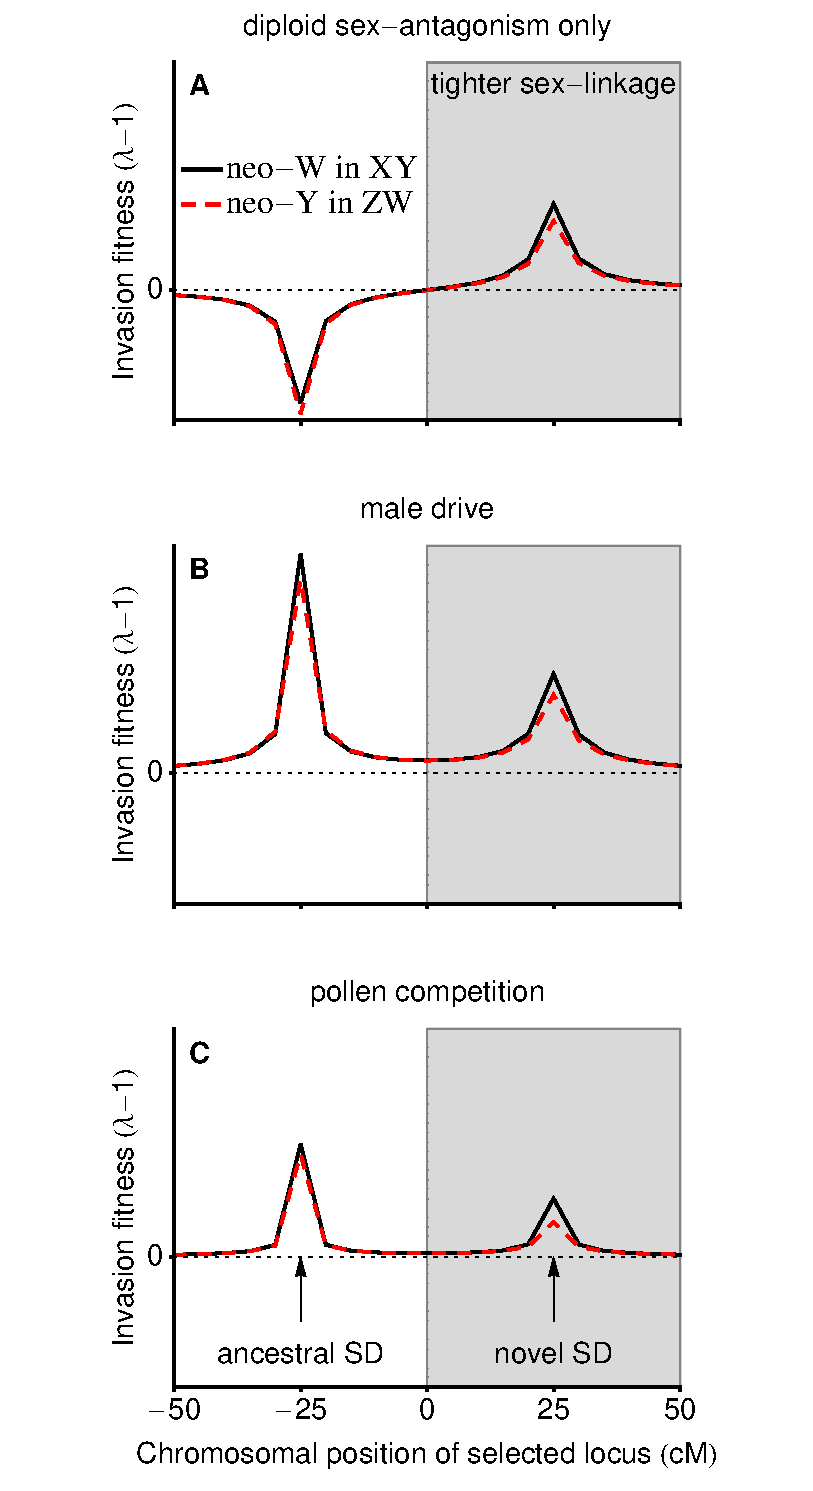
\includegraphics[width=0.5\linewidth]{PositionPlot_4}
%\caption{
% A neo-W can invade an XY system under a large number of selective regimes.
%In panel A, there is no haploid selection ($t^\Hermaphrodite = \alpha^\Hermaphrodite_{\Delta} = 0$) and selection in diploids is sexually antagonistic ($s^\male = -s^\female = 1/10$, $h^\male = 1-h^\female = 3/10$), in which case the neo-sex-determining allele can only invade if it is more closely linked to the selected locus ($R<r$, gray region; but see Figure \ref{fig:SexAntagTighter}B for the case of very tight linkage).
%In panel B, male drive ($\alpha^\male_{\Delta} = -1/20$, $t^\Hermaphrodite = \alpha^\female_{\Delta} = 0$) opposes selection in diploids (no sex-differences: $s^\Hermaphrodite = 1/10$, $h^\Hermaphrodite = 7/10$), in which case the neo-sex-determining allele can invade regardless of linkage.   
%In panel C, haploid competition in males ($t^\male = -1/10$, $t^\female = \alpha^\Hermaphrodite_{\Delta} = 0$) opposes selection in diploids (sex-differences: $s^\male = 3 s^\female = 3/20$, $h^\Hermaphrodite = 7/10$), in which case the neo-sex-determining allele can once again invade regardless of linkage.
%We use Haldane's map function \citep[Equation 3 in ][]{Haldane1919} to convert from map distance (centiMorgans, cM) to the probability of recombination (an odd number of cross-over events).   
%}
%\label{fig:Combination_Centimorgans}
%\end{figure}
%%%%%%%%%%%%%%%%%%%%%%%%%%%%%%%%%%%%%%%%%%%%%%%%%%%%%%%%%
%\newpage

%%%%%%%%%%%%%%%%%%%%%%%%%%%%%%%%%%%%%%%%%%%%%%%%%%%%%%%%%
%Sex-ratio selection is not a good predictor of neo-W invasion into an XY system
%%%%%%%%%%%%%%%%%%%%%%%%%%%%%%%%%%%%%%%%%%%%%%%%%%%%%%%%%
%\begin{figure}[!h]
%\centering
%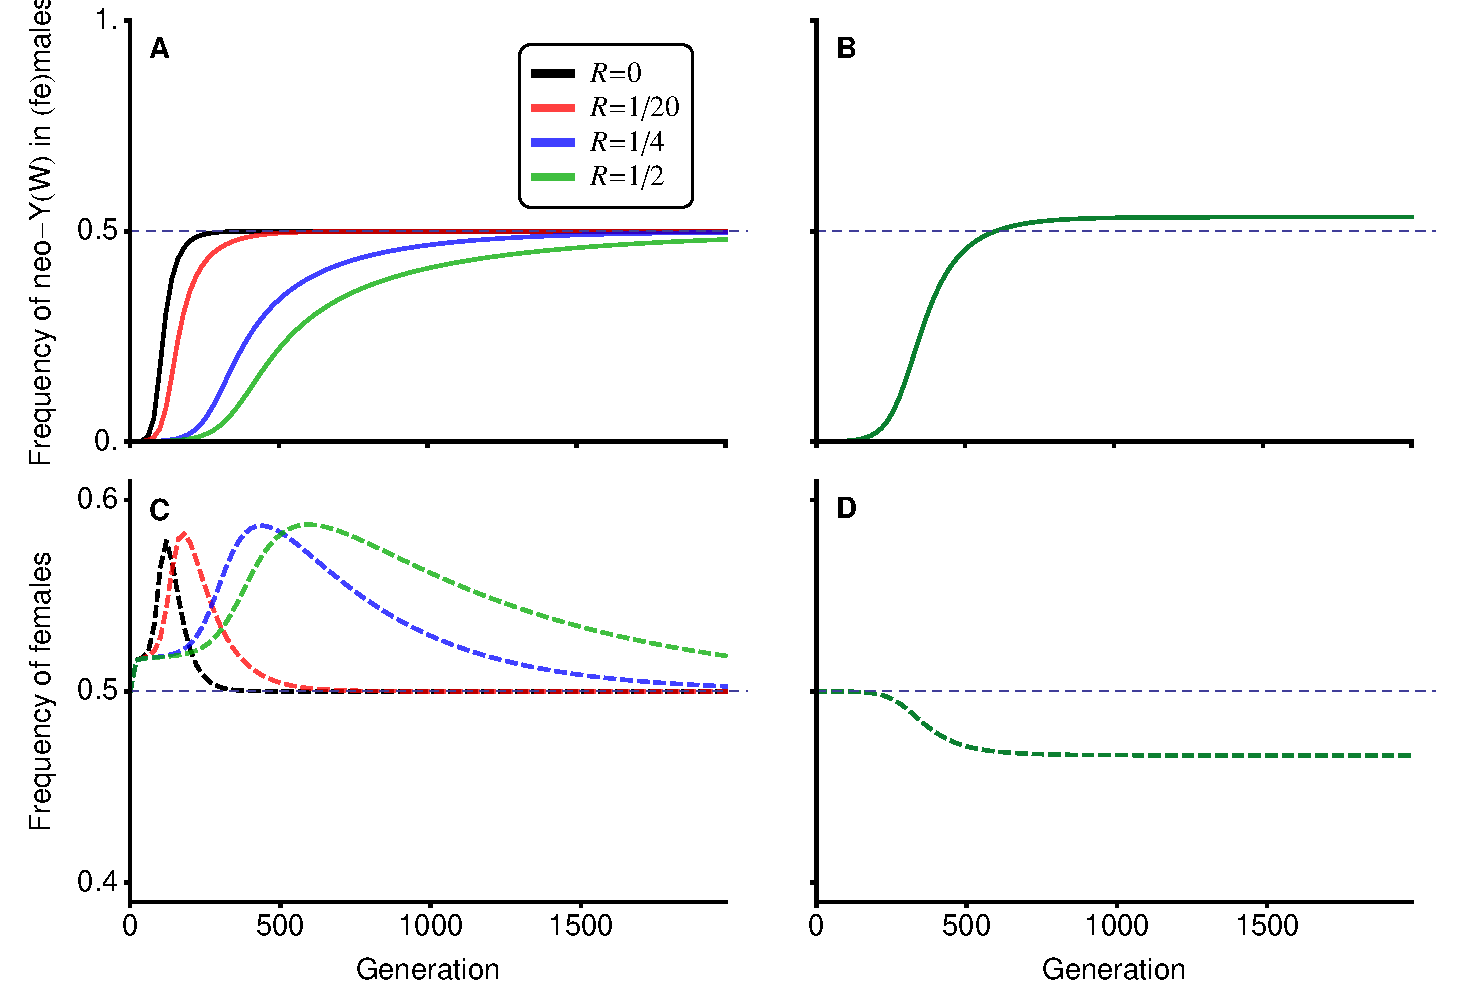
\includegraphics[width=\linewidth]{Combination_Turnover_Ratio}
%\caption{
%Sex-ratio selection alone is not a good predictor of turnover between sex-determining systems.
%In panels A and C, male drive in an ancestral XY system causes a male bias, allowing a neo-W to invade and fix (causing the Y to fix in females), which balances the sex ratio (it also avoids selection in males, and thus makes better females in this case of sex-specific ploidally-antagonistic selection).
%In panels B and D, male drive in an ancestral ZW system has no affect on the sex ratio, yet a neo-Y can invade and fix (causing the W to fix in males) because it becomes linked with the driving allele, and this imparts a sex ratio bias.
%Parameters:  $s^\female =s^\male = 0.2$, $h^\female = h^\male = 0.7$, $t^\female = t^\male = \alpha^\male_\Delta = 0$, $\alpha^\female_\Delta = -1/10$, $r=1/20$.
%}
%\label{fig:SexRatioBad}
%\end{figure}
%%%%%%%%%%%%%%%%%%%%%%%%%%%%%%%%%%%%%%%%%%%%%%%%%%%%%%%%%
%\newpage

%%%%%%%%%%%%%%%%%%%%%%%%%%%%%%%%%%%%%%%%%%%%%%%%%%%%%%%%%
%Haploid selection can lead to polymorphic SD systems 
%%%%%%%%%%%%%%%%%%%%%%%%%%%%%%%%%%%%%%%%%%%%%%%%%%%%%%%%%
%\begin{figure}[!h]
%\centering
%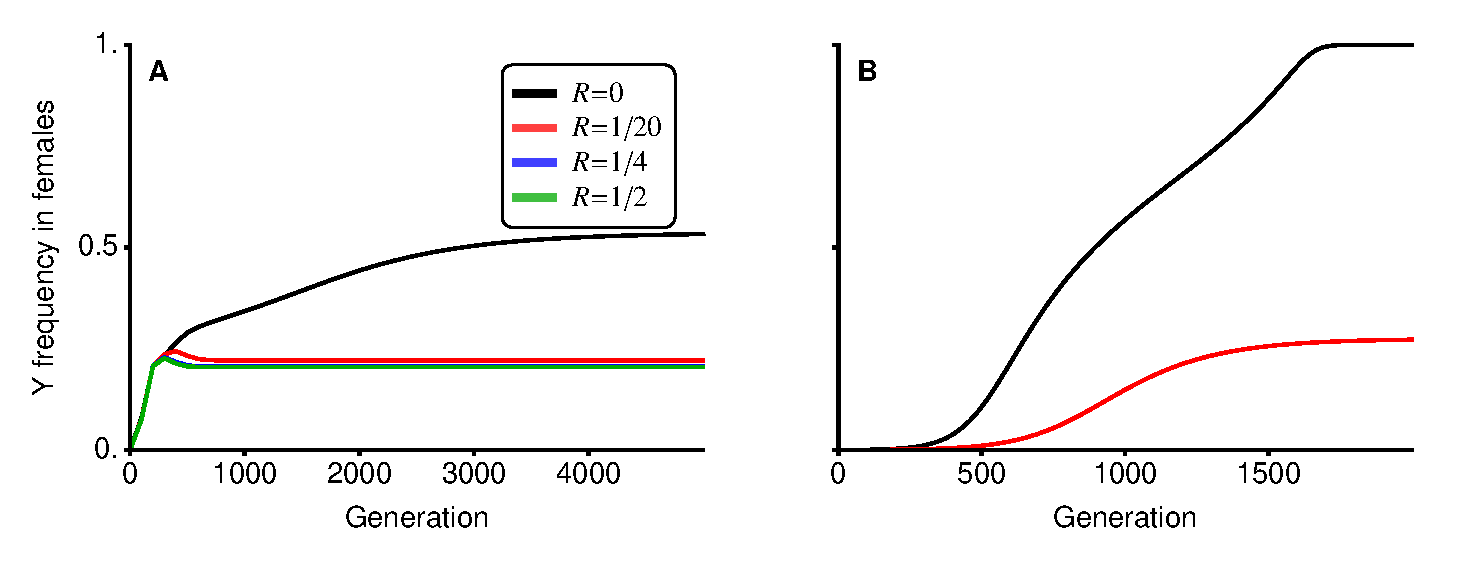
\includegraphics[width=\linewidth]{Polymorphic}
%\caption{
%Tight linkage (relative to selection) and/or haploid selection can cause stable polymorphic sex-determining systems.
%In panel A, there is strong overdominance in both sexes and no haploid selection  (parameters as in Figure \ref{fig:BothOverdominance}B with $r = 1/10$), in which case a neo-W can invade regardless of sex-linkage, but cannot not fix (i.e., the Y does not fix in females, and X, Y, W, and Z all segregate at equilibrium).
%In panel B, there is sex-antagonistic selection at the diploid stage and drive in females (parameters as in Figure \ref{fig:SexAntagTighter} with $\alpha^\female_\Delta = 1/20$ and $r = 1/10$), in which case a sufficiently tightly linked neo-W can invade ($R<\sim r$), but only fixes if $R=0$.   
%}
%\label{fig:Polymorphism}
%\end{figure}
%%%%%%%%%%%%%%%%%%%%%%%%%%%%%%%%%%%%%%%%%%%%%%%%%%%%%%%%%
%\newpage

%%%%%%%%%%%%%%%%%%%%%%%%%%%%%%%%%%%%%%%%%%%%%%%%%%%%%%%%%
%CYCLES!
%%%%%%%%%%%%%%%%%%%%%%%%%%%%%%%%%%%%%%%%%%%%%%%%%%%%%%%%%
%\begin{figure}[!h]
%\centering
%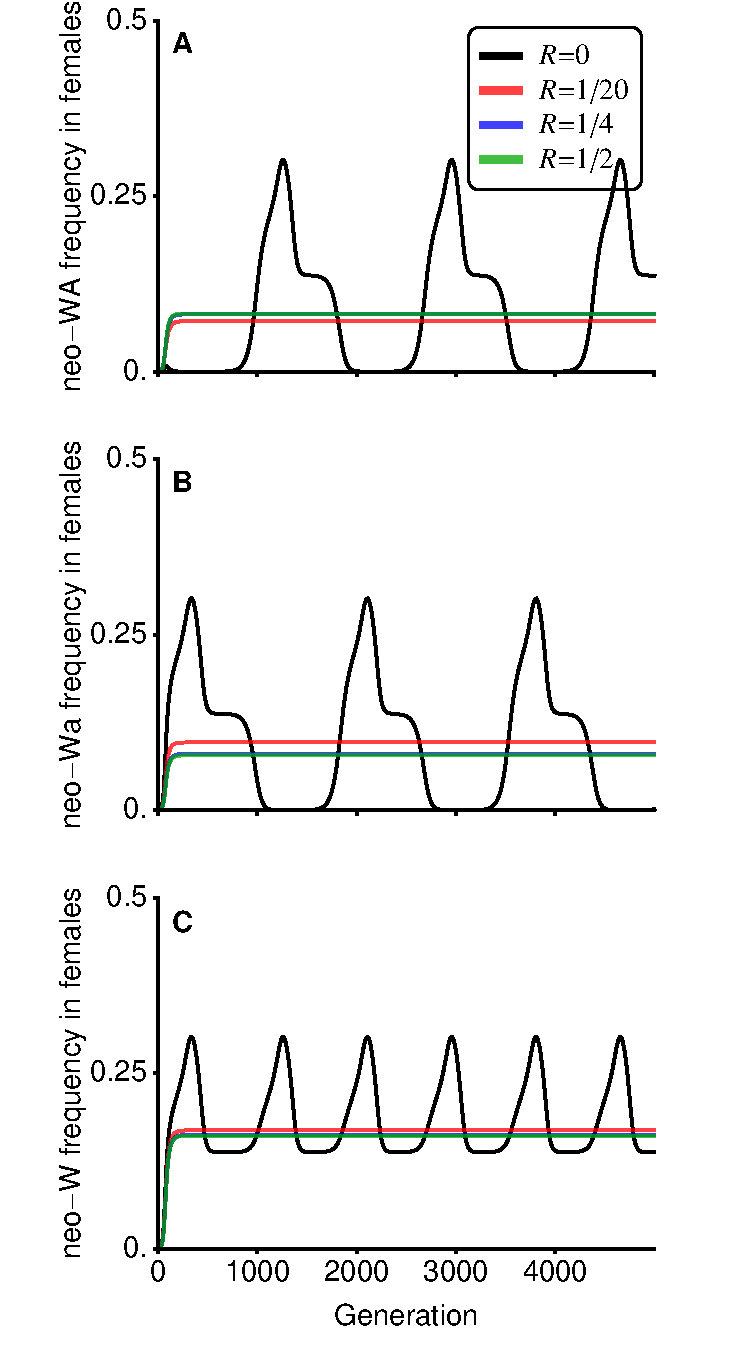
\includegraphics[width=0.5\linewidth]{BothWsInvade_Overdominance_Cycles}
%\caption{
%Thought I'd show this just for fun (not for publication).
%}
%\label{fig:Cycles}
%\end{figure}
%%%%%%%%%%%%%%%%%%%%%%%%%%%%%%%%%%%%%%%%%%%%%%%%%%%%%%%%%
%\newpage

%%%%%%%%%%%%%%%%%%%%%%%%%%%%%%%%%%%%%%%%%%%%%%%%%%%%%%%%%
%Heterogametic transitions with/without sex ratio change
%%%%%%%%%%%%%%%%%%%%%%%%%%%%%%%%%%%%%%%%%%%%%%%%%%%%%%%%%
%\begin{figure}[!h]
%\centering
%\begin{tikzpicture}[remember picture]
%	\node[] (plot) {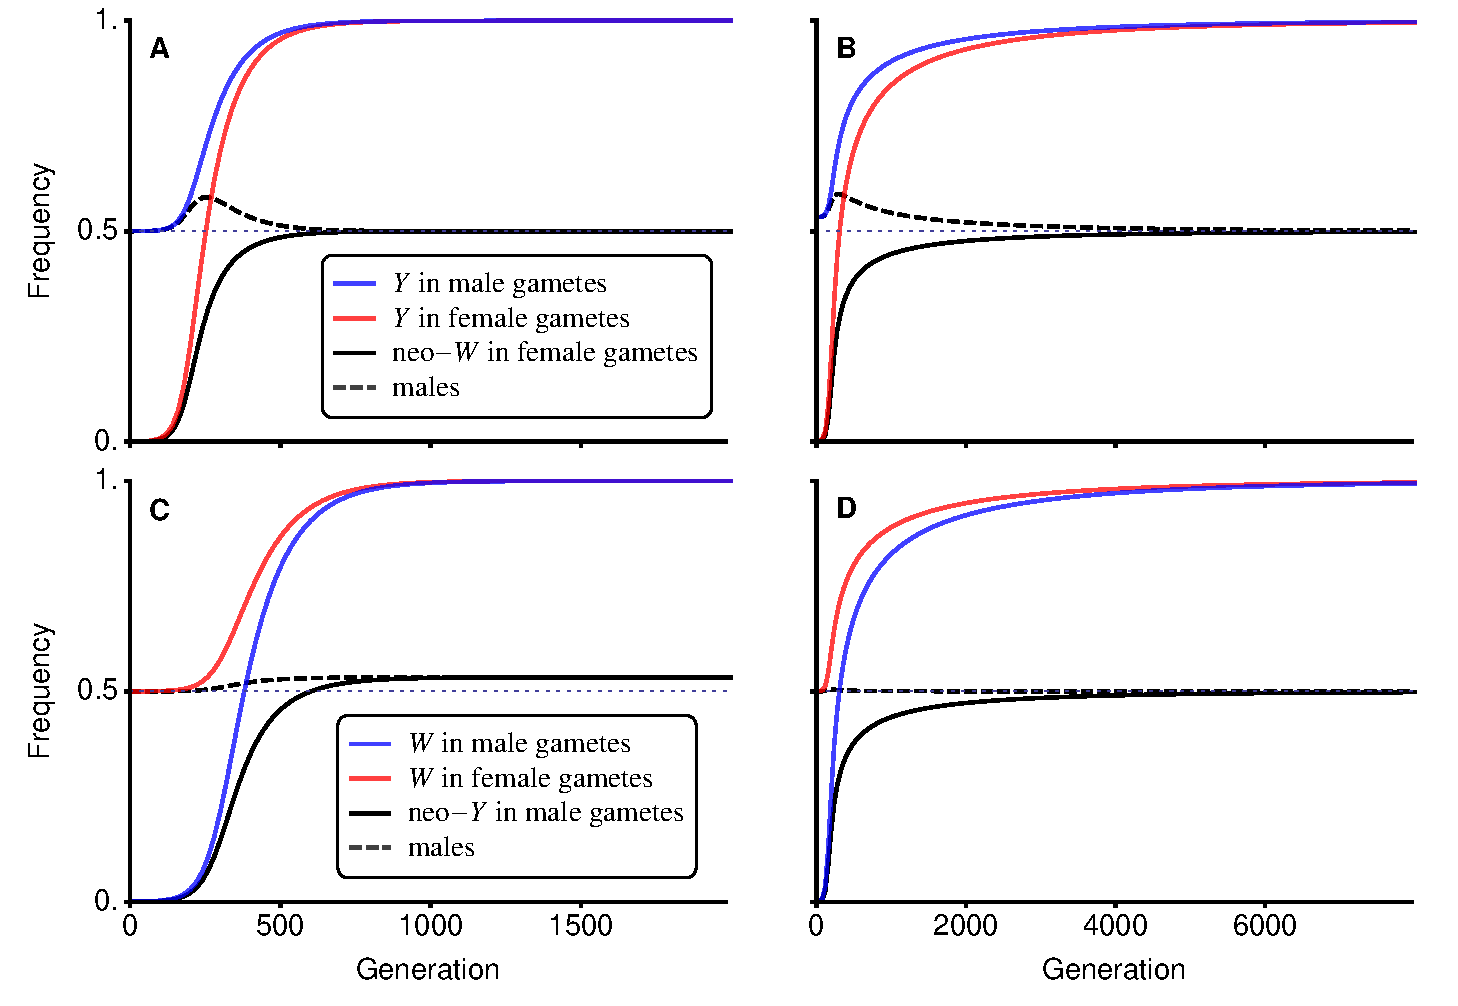
\includegraphics[width=\linewidth]{Combination_Turnover}};
%	\node[above = 0cm of plot, xshift = -70] () {$r=0.5$, $R=0.05$};
%	\node[above = 0cm of plot, xshift = 120] () {$r=0.05$, $R=0.5$};
%	\node[left = 0cm of plot, yshift = 105, rotate = 90] () {XY $\rightarrow$ ZW};
%	\node[left = 0cm of plot, yshift = -20, rotate = 90] () {ZW $\rightarrow$ XY};
%\end{tikzpicture}
%\caption{
%Heterogametic transitions from XY to ZW sex determination (neo-W frequency shown by black lines, panels A and B) or from ZW to XY (neo-Y frequency shown by black lines, panels C and D) occur similarly regardless of sex ratio biases present before (B versus D) or after (C versus A, dashed lines show male frequency). 
%During invasion by a neo-ZW sex-determination system (A and B), the ancestral Y fixes in both males and females (blue and red lines). 
%Similarly, the ancestral W allele fixes in males and females (blue and red lines) during a ZW to XY transition. 
%In this plot, there is no gametic competition ($t^\female=t^\male=0$) and meiotic drive occurs during male meiosis only ($\alpha^\female_{\Delta}=0$, $\alpha^\male_{\Delta}=-1/5$). Therefore, sex ratio biases can only arise when the \textbf{A} locus is linked to an XY sex-determining locus.
%In panels A and C, the neo-sex-determining locus is more closely linked to the \textbf{A} locus than the ancestral sex-detemining region ($r=1/2$, $R=1/20$) such that a neo-Y can caused biased sex ratios (panel C).
%In panels B and D, the ancestral sex-determining locus is more closely linked to the \textbf{A} locus than the neo-sex-detemining locus ($r=1/20$, $R=1/2$). 
%Therefore, an ancestral XY sex determination can have a biased zygotic sex ratio that becomes unbiased after an unlinked neo-W invades (B). 
%However, in panel D, a unlinked neo-Y invades an ancestral ZW sex-determination system in a similar manner but no biases to the zygotic sex ratio occur. 
%With diploid selection alone, neo-sex-determining loci do not spread if they are less closely linked to the \textbf{A} locus than the ancestral sex-determining locus (see equation \eqref{eq:lambda_neoW} and Figure \ref{fig:Combination_Centimorgans}A). 
%In this plot there are no sex differences in selection and an equilibrium is maintained because selection in diploids opposes meiotic drive, $s^\female =s^\male = 1/5$, $h^\female = h^\male = 7/10$.
%\textcolor{red}{Aesthetic adjustments: 
%%Could add titles to the columns/rows: neo-W for row 1, neo-Y for row 3, $r=0.5$, $R=0.05$ for column 1 and $r=0.05$, $R=0.5$ for column 2. 
%%Could adjust padding (too much whitespace where there is no axis label). 
%%It also seems could increase ratio of font size relative to plot size to make figure more compact. 
%%Matt - could you uncomment the line legends in the Mathematica file (function not included in my Mathematica version).
%Add chromosome cartoons to depict recombination rates?
%}
%}
%\label{fig:Combination_Turnover}
%\end{figure}
%%%%%%%%%%%%%%%%%%%%%%%%%%%%%%%%%%%%%%%%%%%%%%%%%%%%%%%%%
%\newpage


%%%%%%%%%%%%%%%%%%%%%%%%%%%%%%%%%%%%%%%%%%%%%%%%%%%%%%%%%
%Heterogametic transitions with/without sex ratio change
%%%%%%%%%%%%%%%%%%%%%%%%%%%%%%%%%%%%%%%%%%%%%%%%%%%%%%%%%
%\begin{figure}[!h]
%\centering
%\begin{tikzpicture}[remember picture]
%	\node[] (plot) {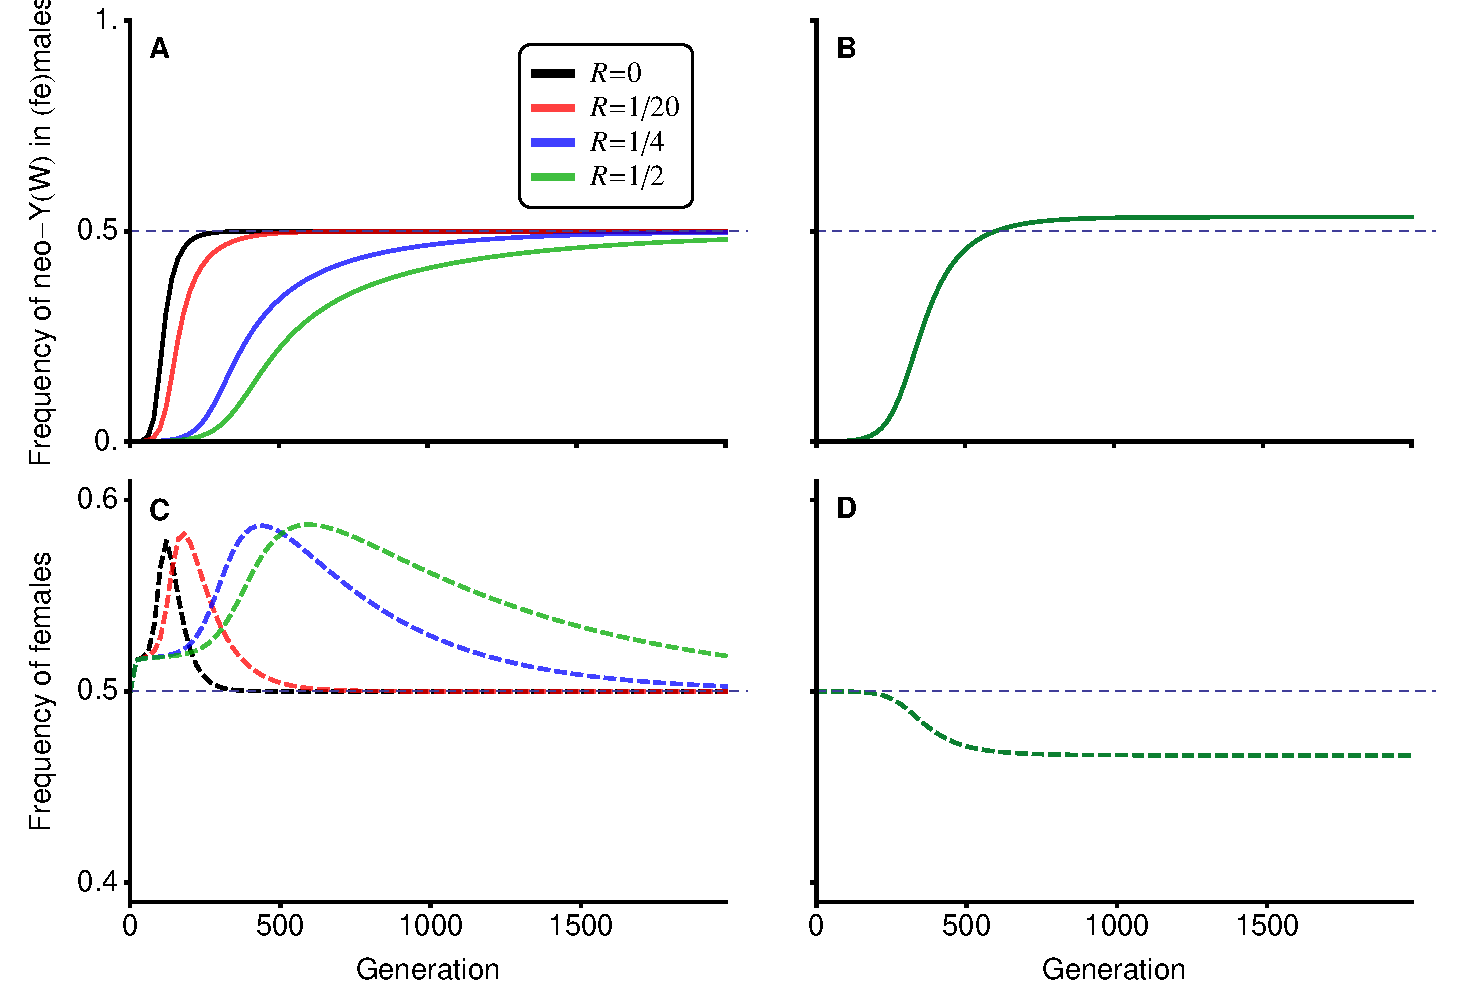
\includegraphics[width=\linewidth]{Combination_Turnover_Ratio}};
%	\node[above = -1cm of plot, xshift = -100] () {XY $\rightarrow$ ZW};
%	\node[above = -1cm of plot, xshift = 90] () {ZW $\rightarrow$ XY};
%\end{tikzpicture}
%\caption{
%%\textcolor{red}{Is this what Sally was thinking?}
%%\textcolor{blue}{I think this works but I'm confused as to why the speed of spread should be so much different for XY and ZW here. Figure \ref{fig:Combination_Turnover} and \ref{fig:Combination_Centimorgans} suggests that there's not much difference between XY->ZW and ZW->XY. Maybe we should just stick with the 4 cases in figure \ref{fig:Combination_Turnover}. }
%%\textcolor{red}{i messed up and had $r=0.5$ instead of $r=0.05$ for B and D. haven't fixed fitness plot below.}
%Heterogametic transitions occur (panels A and B) regardless of sex ratio biases (panels C and D).
%A neo-W invades (panel A) and equalizes the male-biased sex ratio (panel C) that was caused by meiotic drive in males.
%A neo-Y invades (panel B) a population with an equal sex ratio. 
%With any amount of linkage ($R<1/2$), the neo-Y becomes associated with the driving allele in males, and in the end causes a male bias.
%Parameters: $s^\female = s^\male = 1/5$, $h^\female = h^\male = 7/10$, $t^\female = t^\male=0$, $\alpha^\female_\Delta = 0$, $\alpha^\male_\Delta = -1/5$, $r = 1/20$.
%}
%\label{fig:Combination_Turnover_Ratio}
%\end{figure}
%%%%%%%%%%%%%%%%%%%%%%%%%%%%%%%%%%%%%%%%%%%%%%%%%%%%%%%%%%
%\newpage

%%%%%%%%%%%%%%%%%%%%%%%%%%%%%%%%%%%%%%%%%%%%%%%%%%%%%%%%%%
%%Changes in mean fitness
%%%%%%%%%%%%%%%%%%%%%%%%%%%%%%%%%%%%%%%%%%%%%%%%%%%%%%%%%%
%\begin{figure}[!h]
%\centering
%\begin{tikzpicture}[remember picture]
%	\node[] (plot) {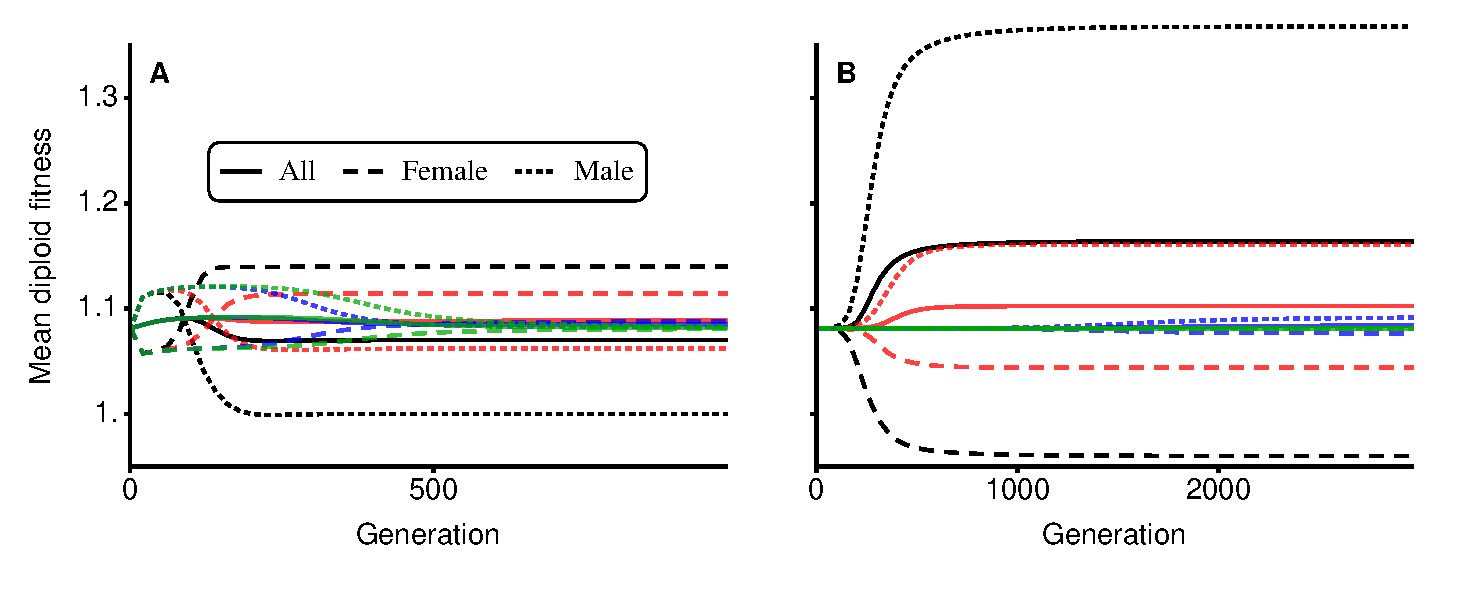
\includegraphics[width=\linewidth]{Combination_Fitness_Rec}};
%	\node[above = -1cm of plot, xshift = -100] () {XY $\rightarrow$ ZW};
%	\node[above = -1cm of plot, xshift = 90] () {ZW $\rightarrow$ XY};
%\end{tikzpicture}
%\caption{
%\textcolor{red}{This complicated thing matches the plot above. I don't think we want to include it...?}
%}
%\label{fig:Combination_Fitness_Rec}
%\end{figure}
%%%%%%%%%%%%%%%%%%%%%%%%%%%%%%%%%%%%%%%%%%%%%%%%%%%%%%%%%%
%\newpage

%%%%%%%%%%%%%%%%%%%%%%%%%%%%%%%%%%%%%%%%%%%%%%%%%%%%%%%%%
%Changes in mean fitness
%%%%%%%%%%%%%%%%%%%%%%%%%%%%%%%%%%%%%%%%%%%%%%%%%%%%%%%%%
%\begin{figure}[!h]
%\centering
%\begin{tikzpicture}[remember picture]
%	\node[] (plot) {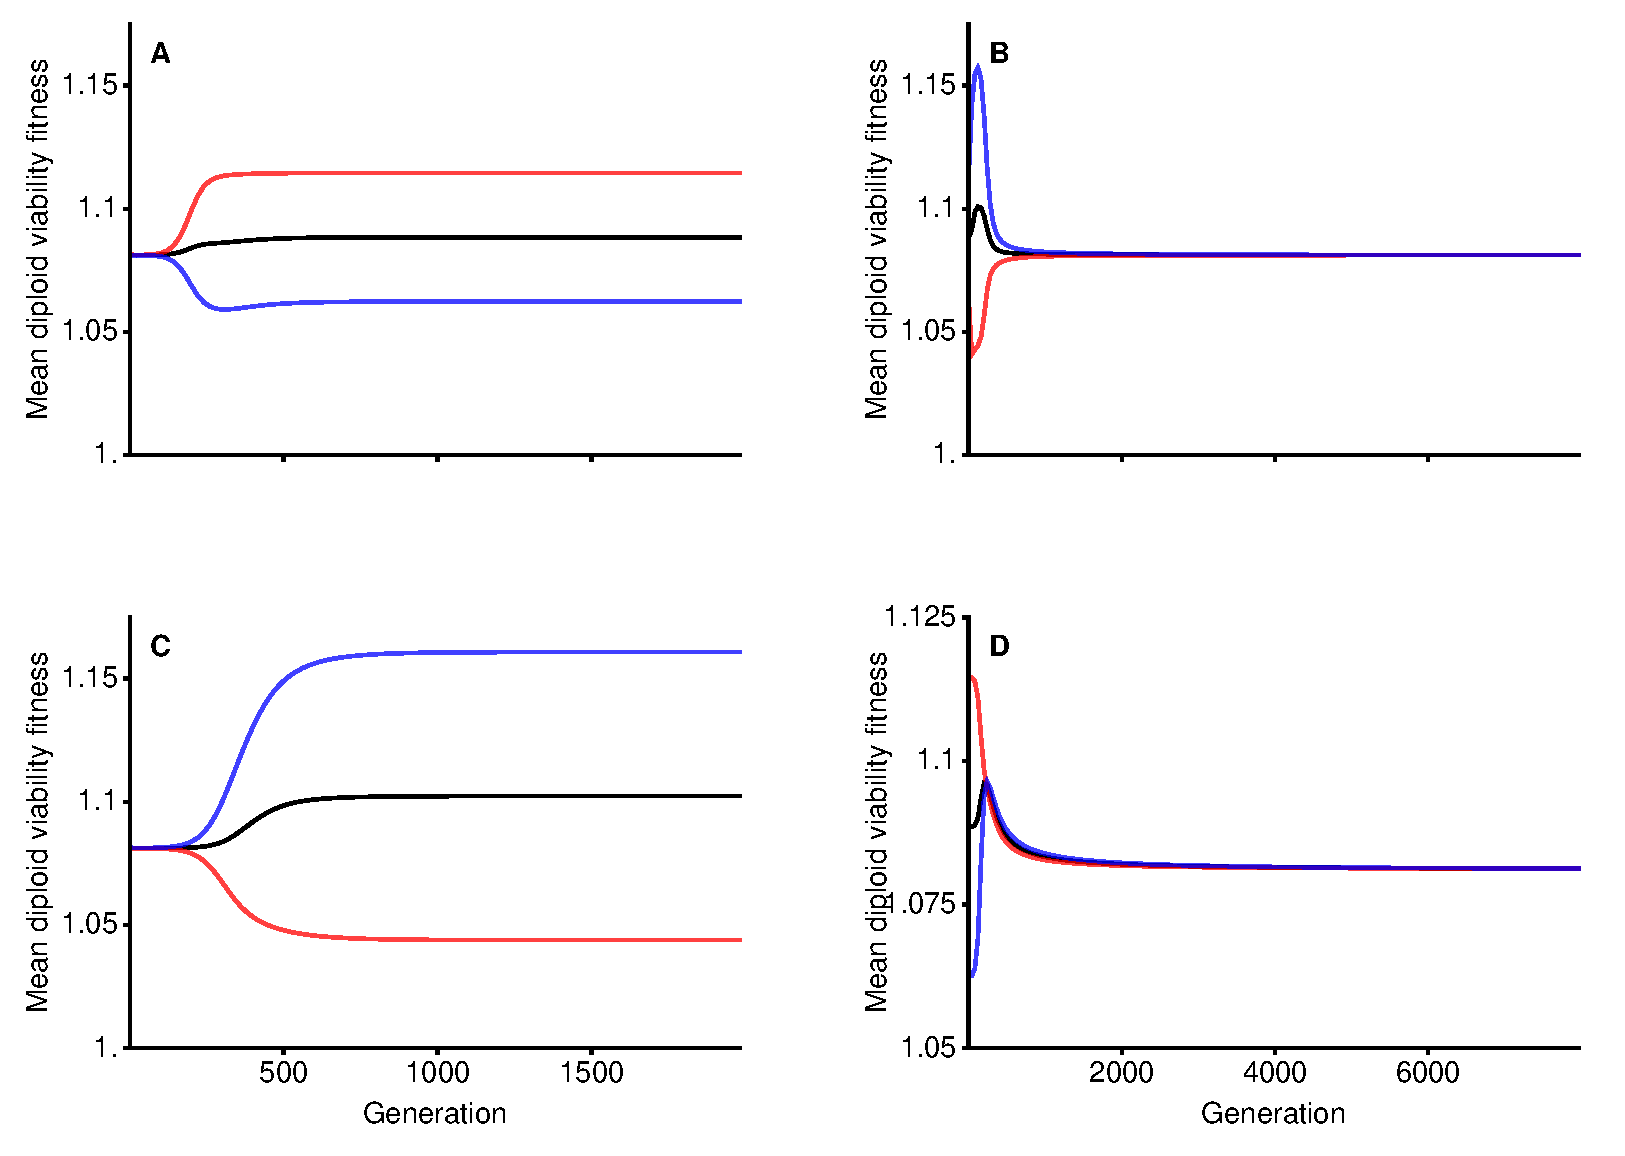
\includegraphics[width=\linewidth]{Combination_MeanFit}};
%	\node[above = 0cm of plot, xshift = -70] () {$r=0.5$, $R=0.05$};
%	\node[above = 0cm of plot, xshift = 120] () {$r=0.05$, $R=0.5$};
%	\node[left = 0cm of plot, yshift = 105, rotate = 90] () {XY $\rightarrow$ ZW};
%	\node[left = 0cm of plot, yshift = -20, rotate = 90] () {ZW $\rightarrow$ XY};
%\end{tikzpicture}
%\caption{
%Changes in mean diploid fitness of males (blue lines), females (red lines), and the entire population (black lines) during the transitions between sex-determination systems shown in Figure \ref{fig:Combination_Turnover}. 
%Here mean diploid fitness of a particular sex is its mean diploid viability fitness times twice its frequency in the population, to capture the fact that epistatically dominant sex-determining alleles can also invade because they selfishly make more of the sex they are in. 
%The mean fitness of females increases during the spread of neo-W alleles (A and B) and the mean fitness of males increases during the spread of neo-Y alleles (C and D). 
%However, when a neo-sex determining system evolves that is less closely linked to a locus under selection (B and D), population mean fitness decreases. 
%%\textcolor{red}{
%%Could add titles to the columns/rows: neo-W for row 1, neo-Y for row 3, $r=0.5$, $R=0.05$ for column 1 and $r=0.05$, $R=0.5$ for column 2. 
%%%\& possibly adjust padding (too much whitespace?). 
%%%Matt - could you uncomment the line legends in the Mathematica file (function not included in my Mathematica version).
%%}
%%\textcolor{red}{I'm still confused why male and female mean fitnesses aren't normalized by their frequency. I'm not sure we should be calling them means without this normalization step. Or we should justify this by saying that mean fitness also has something to do with the number of a sex, i.e., multiply *real* mean fitness in females by freqfemale/(1/2)? See the next figure for what happens when we do normalize.}
%\textcolor{blue}{I think we should give this plot showing (male mean fitness * freq males) and (female mean fitness * freq females), without multiplying by 2 (leave off black lines, population mean fitness). 
%We could also re-plot the sex ratios on this same scale. 
%The plot below, `adjusted for sex ratio', could then go in the appendix. The point is that neo-W (neo-Y) can invade when the frequency of females (males) multiplied by their mean fitness increases.  }
%}
%\label{fig:Combination_MeanFit}
%\end{figure}
%%%%%%%%%%%%%%%%%%%%%%%%%%%%%%%%%%%%%%%%%%%%%%%%%%%%%%%%%%
%\newpage

%%%%%%%%%%%%%%%%%%%%%%%%%%%%%%%%%%%%%%%%%%%%%%%%%%%%%%%%%
%Changes in mean fitness corrected for sex ratio
%%%%%%%%%%%%%%%%%%%%%%%%%%%%%%%%%%%%%%%%%%%%%%%%%%%%%%%%%
%\begin{figure}[!h]
%\centering
%\begin{tikzpicture}[remember picture]
%	\node[] (plot) {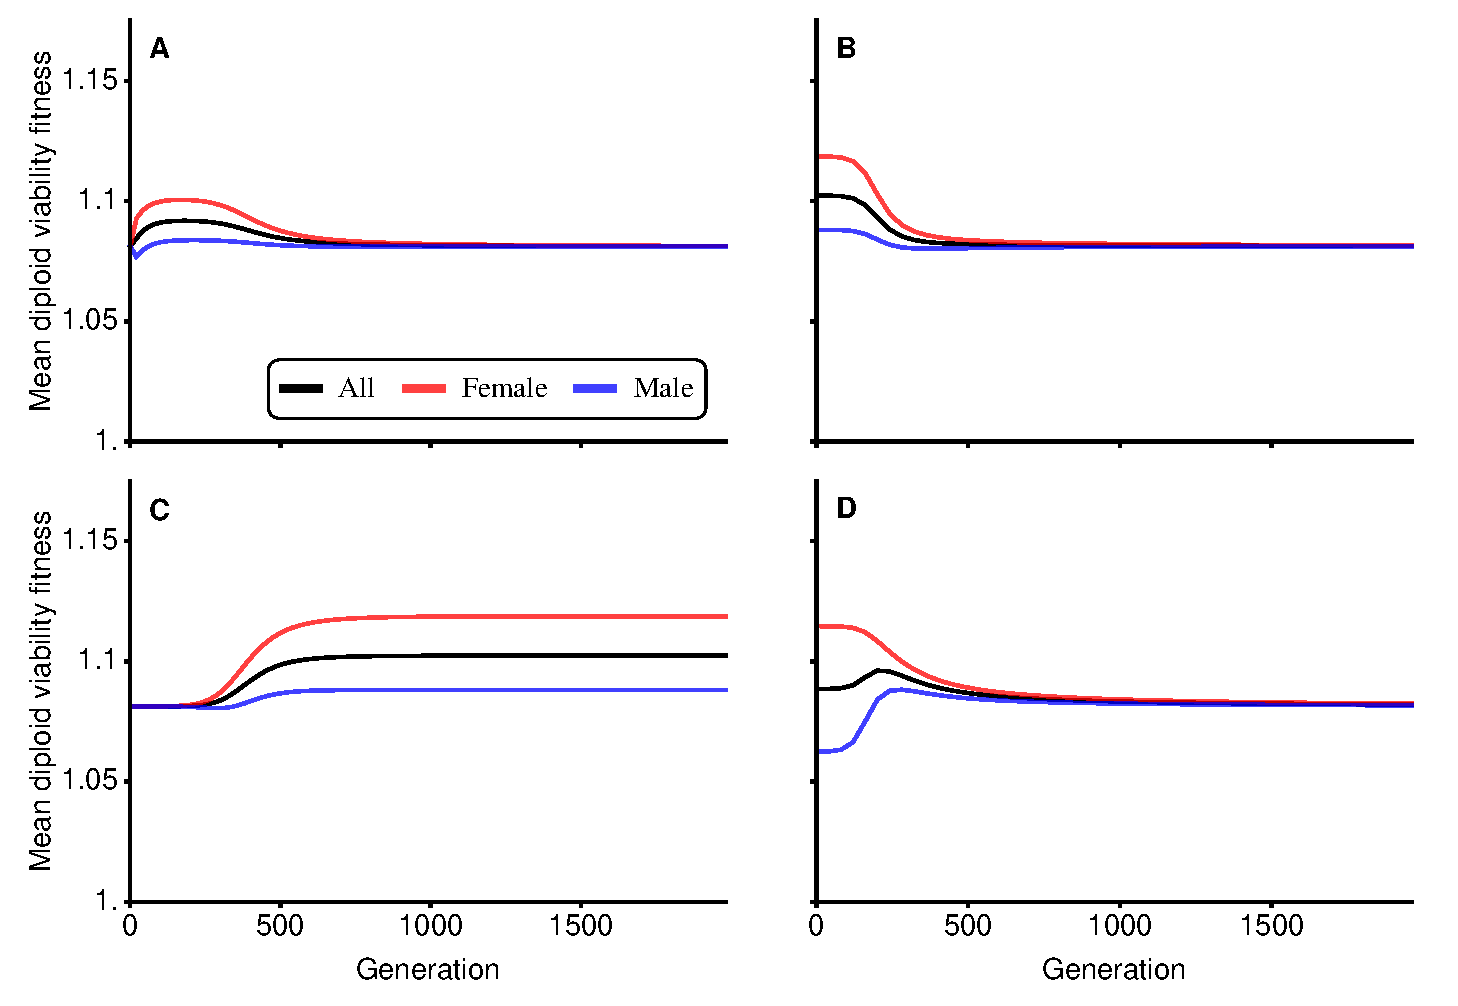
\includegraphics[width=\linewidth]{Combination_MeanFit_Corrected}};
%\end{tikzpicture}
%\caption{
%\textcolor{red}{Last plot with mean fitness of sexes corrected for sex ratio. Could add to previous plot with dashed lines?}
%}
%\label{fig:Combination_MeanFit_Corrected}
%\end{figure}
%%%%%%%%%%%%%%%%%%%%%%%%%%%%%%%%%%%%%%%%%%%%%%%%%%%%%%%%%%
%\newpage

%%%%%%%%%%%%%%%%%%%%%%%%%%%%%%%%%%%%%%%%%%%%%%%%%%%%%%%%%
%%Chromosomal Positions
%%%%%%%%%%%%%%%%%%%%%%%%%%%%%%%%%%%%%%%%%%%%%%%%%%%%%%%%%%
%\begin{figure}[!h]
%\centering
%%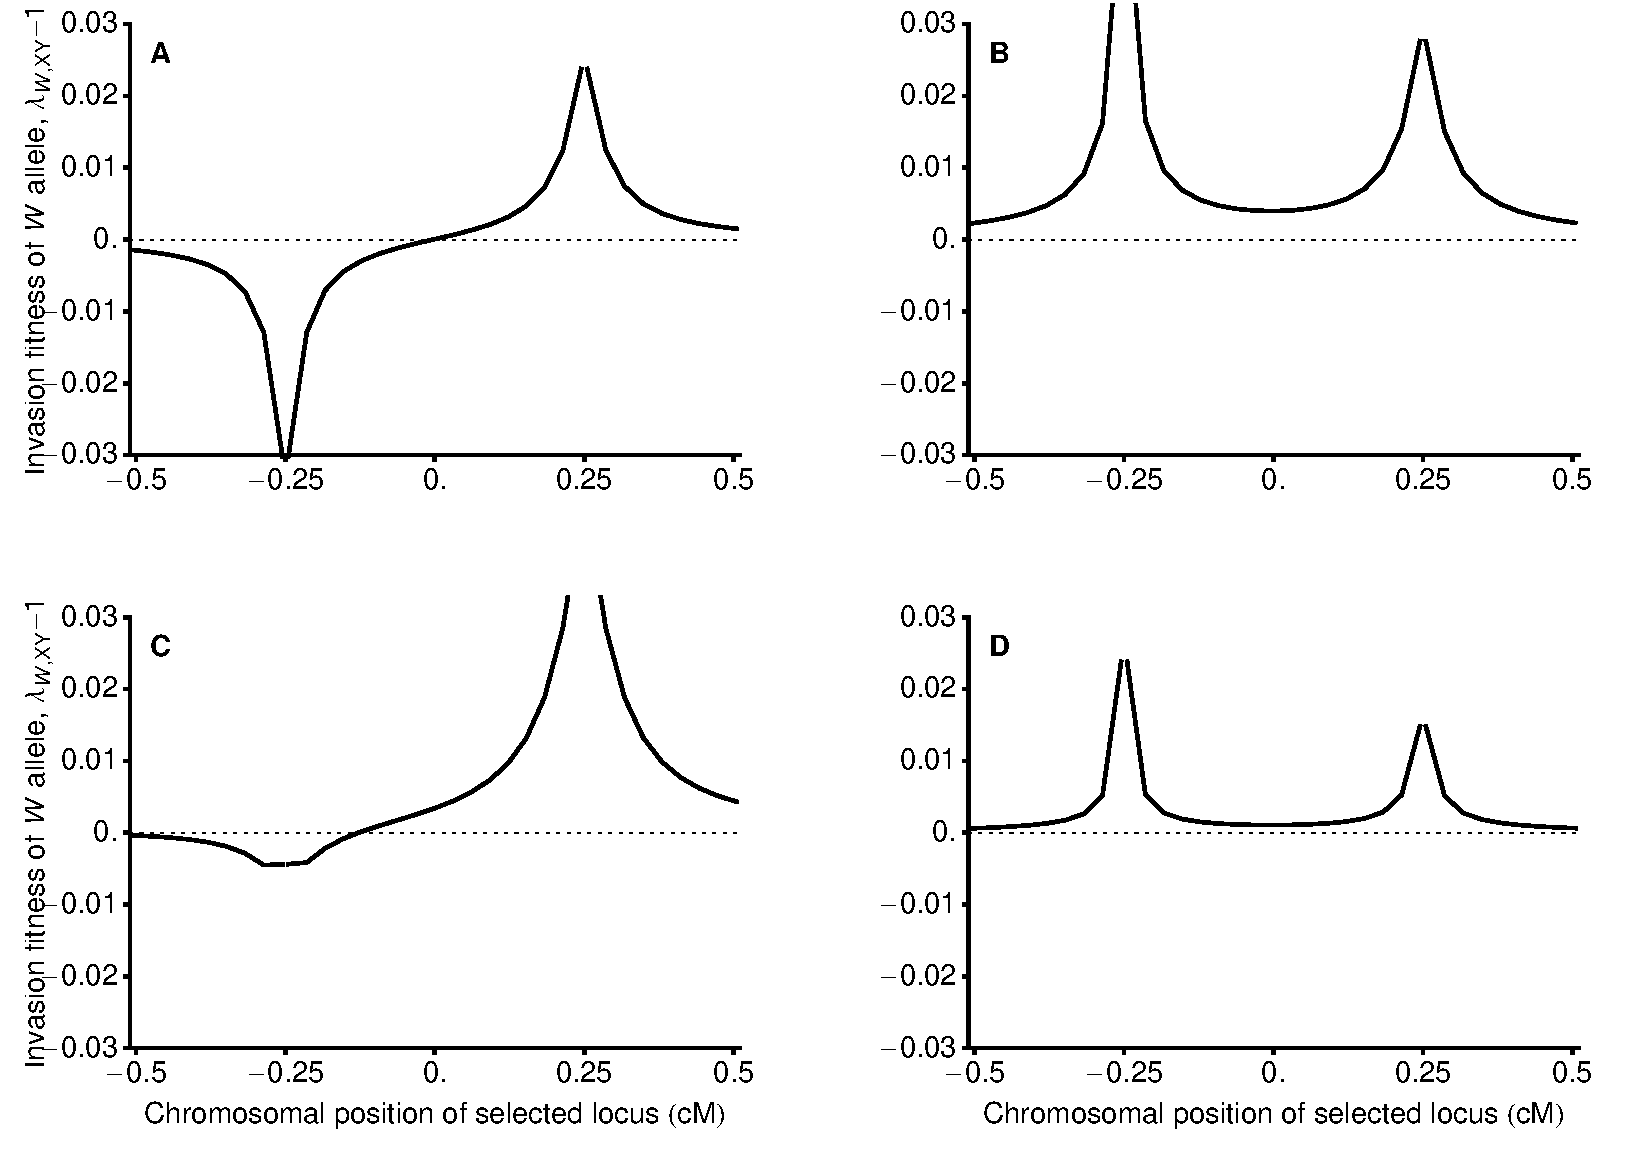
\includegraphics[width=\linewidth]{Combination_Centimorgan}\\
%%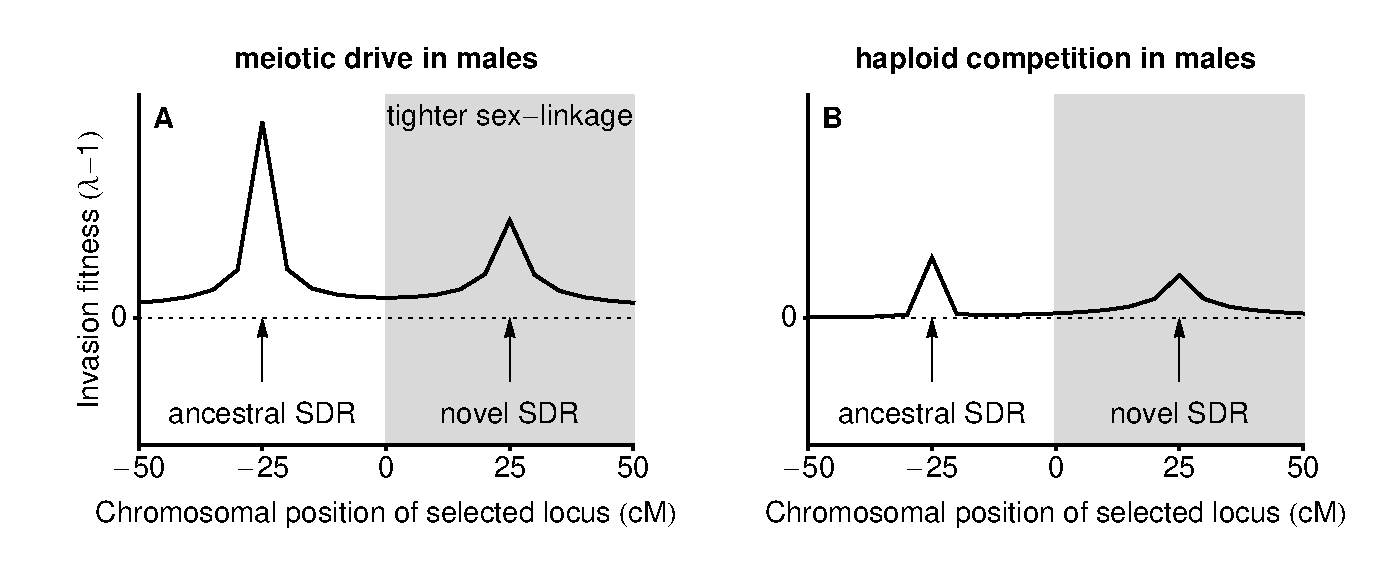
\includegraphics[width=\linewidth]{PositionPlot}\\
%\begin{tikzpicture}[remember picture]
%%	\node[] () {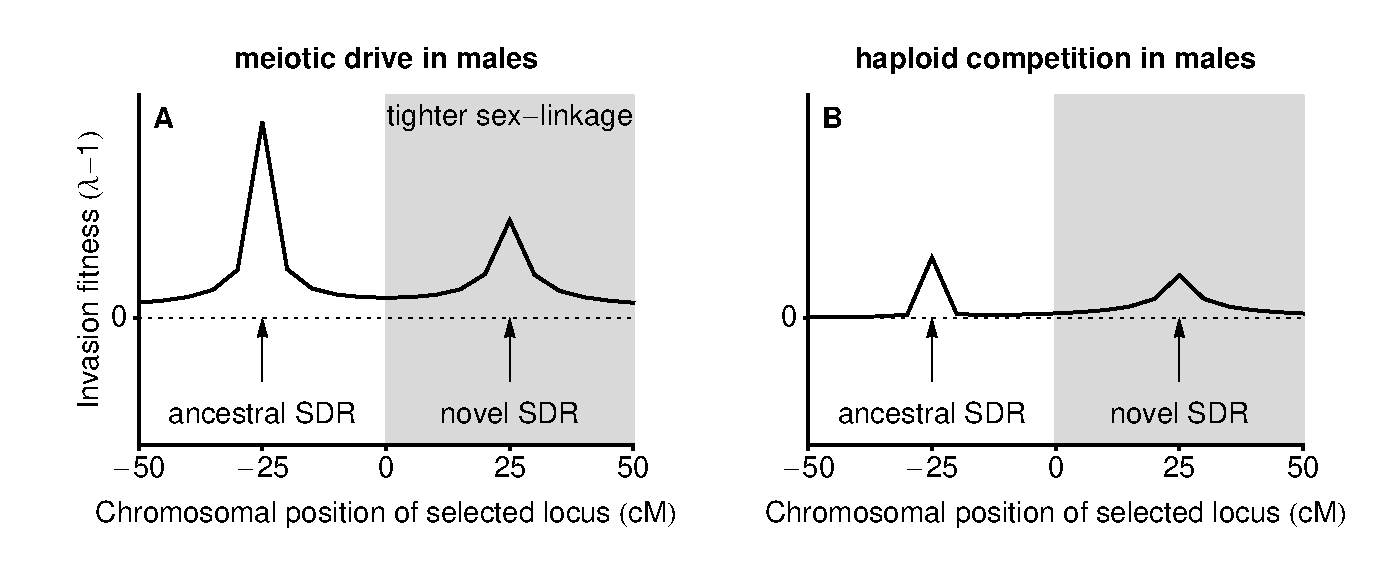
\includegraphics[width=\linewidth]{PositionPlot}};
%	\node[] () {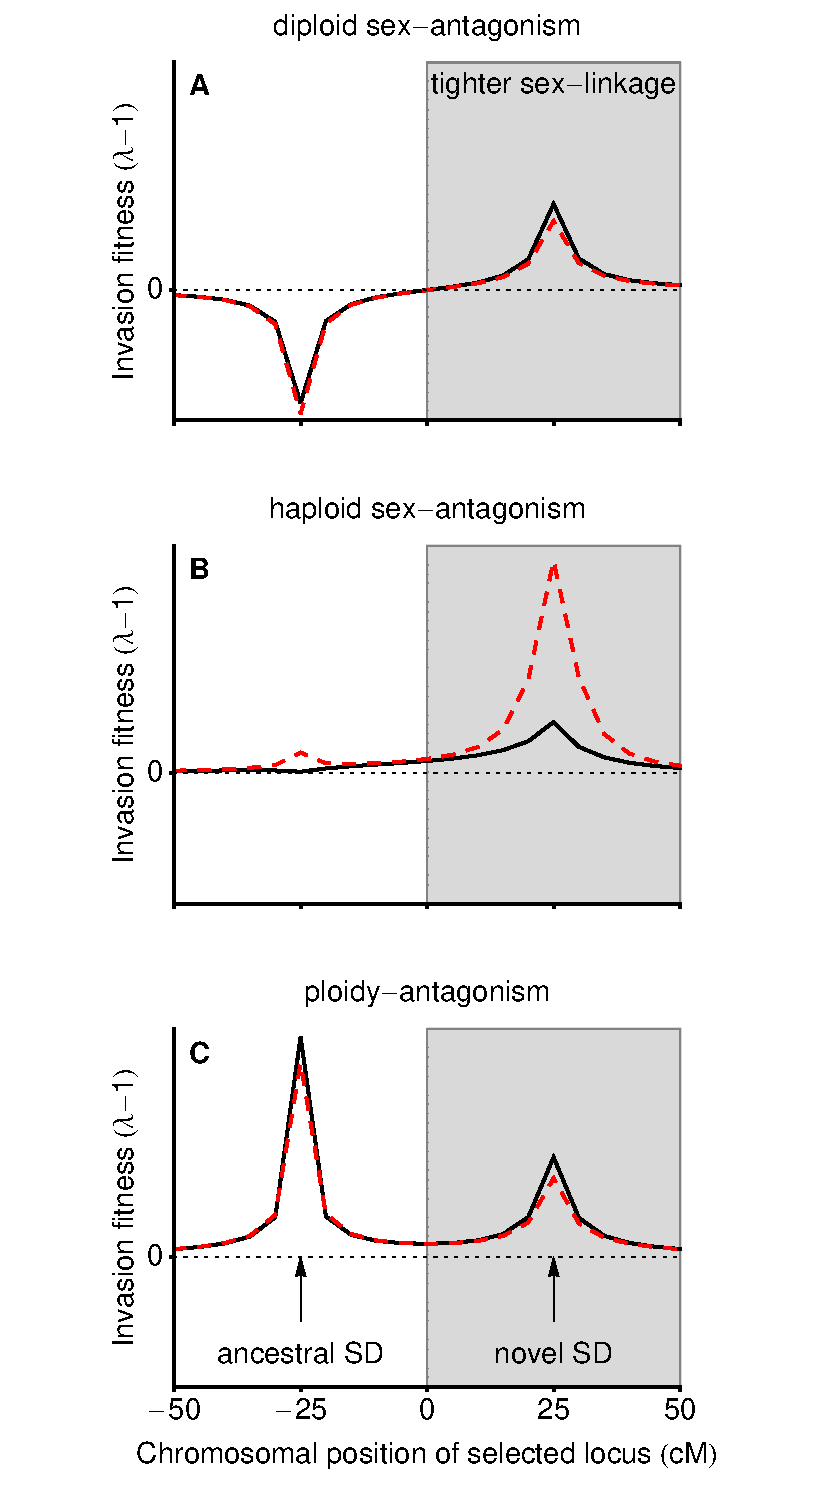
\includegraphics[width=0.5\linewidth]{PositionPlot_2}};
%%	\node[anchor=east] at (0, 1.5) {\footnotesize diploid sex-antagonism}; %, $s^\male s^\female < 0$};
%%	\node[anchor=east] at (6.5, 1.5) {\footnotesize haploid sex-antagonism}; %, $s^\male s^\female > 0$};
%%	\node[anchor=east] at (0, -3) {\footnotesize male drive (ploidy-antagonism)}; %, $s^\male < s^\female$};
%%	\node[anchor=east] at (6.5, -3) {\footnotesize find something interesting to plot};%, $s^\female < s^\female$};
%%	\node[anchor=center] at (-1.3, 4.25) {\scriptsize tighter sex-linkage};
%%	\node[anchor=center] at (2.45, 3.5) {\scriptsize ancestral SDR};
%%	\draw[->,thick] (2.45, 3.25) -- (2.45, 2.5);
%%	\node[anchor=center] at (-1.4, -0.25) {\scriptsize novel SDR};
%%	\draw[->,thick] (-1.4, -0.5) -- (-1.4, -1);
%\end{tikzpicture}
%\caption{
% A neo-W can invade an XY system under a large number of selective regimes.
%%Invasion fitness of a neo-sex-determining allele against the relative genomic location of a locus under direct selection. 
%% (neo-Y invading ZW in black, neo-W invading XY in red)
%%The ancestral sex-determining locus is located at -25 and the novel sex-determining locus is located at 25. %and that there is a polymorphism at the \textbf{A} locus maintained by selection.
%%Thus, if the neo-sex-determining allele invades in the gray region the system evolves tighter sex-linkage.  
%In panel A, there is no haploid selection ($t^\Hermaphrodite=\alpha^\Hermaphrodite_{\Delta}=0$) and selection in diploids is sexually antagonistic ($s^\male=-s^\female=1/10$, $h^\male=1-h^\female=3/10$), in which case the neo-sex-determining allele can only invade if it is more closely linked to the selected locus ($R<r$, gray region; but see Figure \ref{fig:SexAntagTighter}B).
%In panel B, there is no diploid selection ($s^\Hermaphrodite=0$) and selection in haploids is sexually antagonistic ($t^\male=-t^\female=0.08$, $\alpha^\Hermaphrodite_{\Delta}=0$), in which case the neo-sex-determining allele can invade regardless of linkage.   
%In panel C, selection in diploids ($s^\male=s^\female=1/10$, $h^\male=h^\female=7/10$) opposes drive in males ($\alpha^\male_{\Delta}=-0.05$, $t^\Hermaphrodite=\alpha^\female_{\Delta}=0$), in which case the neo-sex-determining allele can once again invade regardless of linkage.
%We use Haldane's map function \citep[Equation 3 in ][]{Haldane1919} to convert from map distance (centiMorgans, cM) to the probability of a cross-over event.    
%%we include haploid selection. %and assume that selection in diploids is not sexually-antagonistic ($s^\female s^\male>0$). 
%%A polymorphism can then be maintained by opposing selection between the haploid and diploid phases. 
%%In B, there is drive in favour of the $a$ allele in males ($\alpha^\male_{\Delta}=-1/20$), no female meiotic drive or gametic competition, $t^\Hermaphrodite=\alpha^\female_{\Delta}=0$), and equal selection in diploid sexes ($s^\female=s^\male=1/10$, $h^\female=h^\male=7/10$). 
%%In this case, a neo-W can invade even when the selected locus is more closely linked to the ancestral sex determining locus (see Table \ref{tab:specialcases} and Figure \ref{fig:Combination_Turnover}). 
%%In C and D, there is gametic competition among male gametes only (favouring $a$, $t^\male=-1/10$) and no meiotic drive or gametic competition in females ($t^\female=\alpha^\Hermaphrodite_{\Delta}=0$). 
%%In this case, the neo-W does not invade if $s^\female>s^\male$ (panel C: $s^\female=3/20$, $s^\male=1/20$) but does if $s^\female<s^\male$ (panel D: $s^\female=1/20$, $s^\male=3/20$), see Table \ref{tab:specialcases}.\\ 
%%\textcolor{red}{
%%1. I suspect that panel C has a region where no equilibrium is maintained (CHECK! Maybe include different parameters here or remove the part when no equilibrium). MMO: If you trust the sieve function there are stable equilibria across the entire range, although they differ greatly between XY and ZW systems near -25cM.
%%\\
%%2. Currently use different parameters for B than using in figure \ref{fig:Combination_Turnover} (selection/drive twice as strong in turnover figure). MMO: this is to keep it within the bounds of the plot -- using the same parameters as figure 1 makes the peak at -25 reach roughly 0.1, and then it is difficult to see the details of A,C, and D.
%%%This plot would also benefit from titles giving, e.g., ``sexually-antagonistic selection, $s^\female s^\male<0$'' for A, ``male meiotic drive, $s^\female s^\male>0$'' for B
%%}
%}
%\label{fig:Combination_Centimorgans}
%\end{figure}
%%%%%%%%%%%%%%%%%%%%%%%%%%%%%%%%%%%%%%%%%%%%%%%%%%%%%%%%%%
%\newpage

%%%%%%%%%%%%%%%%%%%%%%%%%%%%%%%%%%%%%%%%%%%%%%%%%%%%%%%%%%
%%Haplotype invasion region plot
%%%%%%%%%%%%%%%%%%%%%%%%%%%%%%%%%%%%%%%%%%%%%%%%%%%%%%%%%%
%\begin{figure}[!h]
%\centering
%\begin{tikzpicture}[remember picture]
%	\node[] () {
%	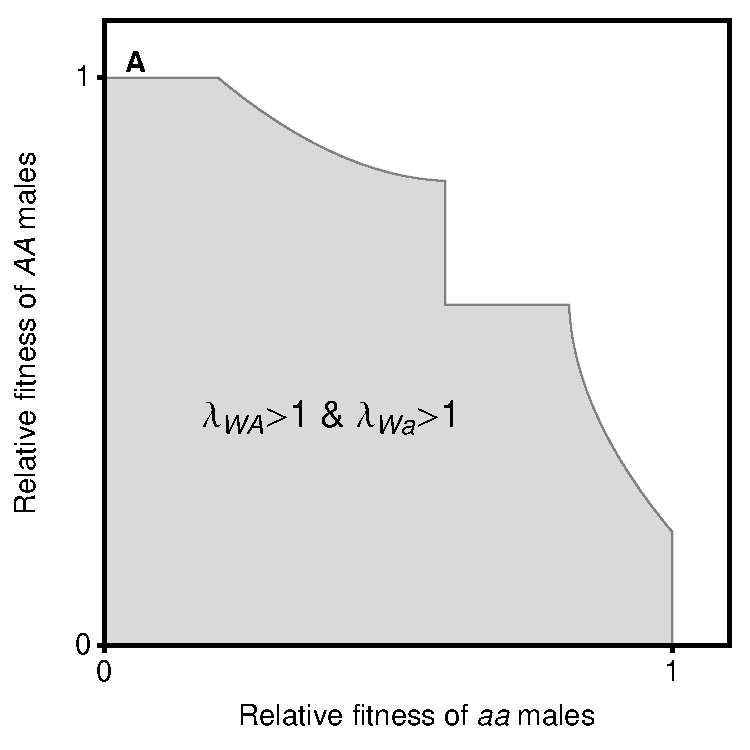
\includegraphics[width=0.5\linewidth]{regionplot_2a}
%	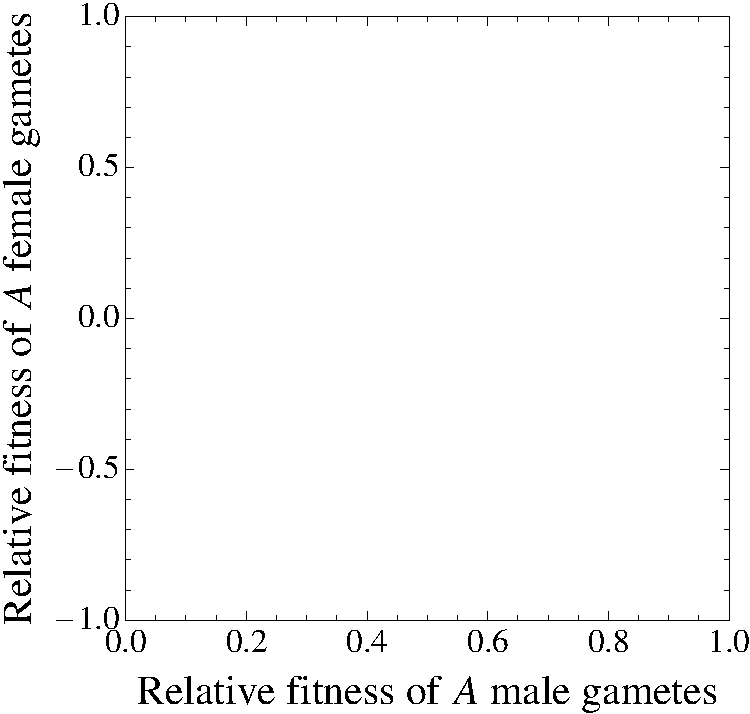
\includegraphics[width=0.5\linewidth]{regionplot_hap}
%	};
%\end{tikzpicture}
%\caption{
%Parameter space (gray) where both neo-W haplotypes can invade from the same stable resident $r=0$ equilibria (equations \ref{eq:tightequil}), and therefore where an unlinked neo-W can invade an XY system with perfect sex-linkage.
%\textbf{A}, In the absence of haploid selection, both neo-W haplotypes can invade for much of the parameter space where the relative fitnesses of male homozygotes, $w_{AA}^\male$ and $w_{aa}^\male$, are both less than that of the heterozygote, $w_{Aa}^\male = 1$.
%In the white region neo-W haplotypes paired with the allele fixed on the Y cannot invade.
%Parameters as in \cite{Otto2014} Figure 2a: $w_A^\Hermaphrodite=w_a^\Hermaphrodite$, $\alpha^\Hermaphrodite=1/2$, $w_{Aa}^\Hermaphrodite=1$, and $w_{AA}^\female=w_{aa}^\female=0.75$.
%\textbf{B}, When selection is the same in both diploid sexes ($w_{aa}^\Hermaphrodite = 1$, $w_{Aa}^\Hermaphrodite = 1 + h s$, $w_{AA}^\Hermaphrodite = 1+s$), both neo-W haplotypes can invade over a portion of the parameter space where selection in diploids ($s$) opposes the force of drive during meiosis in males ($\alpha_{\Delta}^\male$).
%Parameters: $w_A^\Hermaphrodite=w_a^\Hermaphrodite$, $\alpha^\female=1/2$, $h=1/2$.
%}
%\label{fig:regionplot_2a}
%\end{figure}
%%%%%%%%%%%%%%%%%%%%%%%%%%%%%%%%%%%%%%%%%%%%%%%%%%%%%%%%%%
%\newpage

%%%%%%%%%%%%%%%%%%%%%%%%%%%%%%%%%%%%%%%%%%%%%%%%%%%%%%%%%
%W invades XY and fixes
%%%%%%%%%%%%%%%%%%%%%%%%%%%%%%%%%%%%%%%%%%%%%%%%%%%%%%%%%
%\begin{figure}
%\centering
%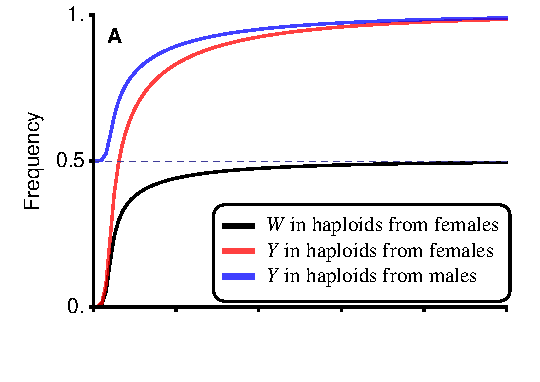
\includegraphics[width=0.5\linewidth]{FreqWLowR}\\
%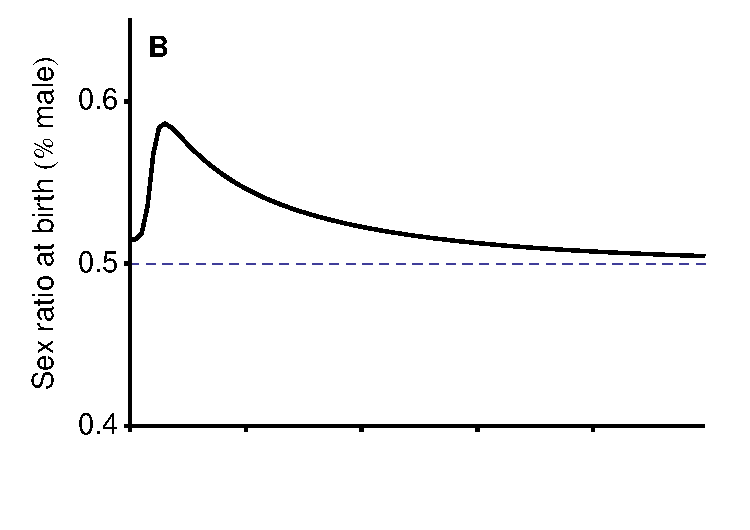
\includegraphics[width=0.5\linewidth]{SexRatioLowR}\\
%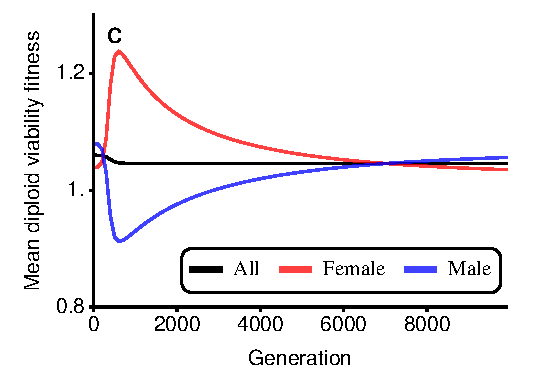
\includegraphics[width=0.5\linewidth]{MeanDipFitLowR}
%\caption{
%Haploid selection allows a neo-$W$ to invade an ancestral $XY$ system and fix (\textbf{A}) despite temporarily biasing the sex ratio further (\textbf{B}) and decreasing mean diploid viability fitness (\textbf{C}).
%Complete turnover between genetic sex-determination systems occurs despite the neo-$W$ being less tightly linked to the selected locus than the ancestral sex-determining locus is, $R>r$.
%Parameters: $k=1$, $s^\female = 0.05$, $s^\male = 0.15$, $h^\female = h^\male = 0.7$, $t^\female = 0$, $t^\male = -0.1$, $\alpha^\male = \alpha^\female = 1/2$, $r=0.01$, $R=0.05$.
%}
%\label{fig:WinvasionLowR}
%\end{figure}
%%%%%%%%%%%%%%%%%%%%%%%%%%%%%%%%%%%%%%%%%%%%%%%%%%%%%%%%%

%%%%%%%%%%%%%%%%%%%%%%%%%%%%%%%%%%%%%%%%%%%%%%%%%%%%%%%%%
%W invades XY but does not fix
%%%%%%%%%%%%%%%%%%%%%%%%%%%%%%%%%%%%%%%%%%%%%%%%%%%%%%%%%
%\begin{figure}
%\centering
%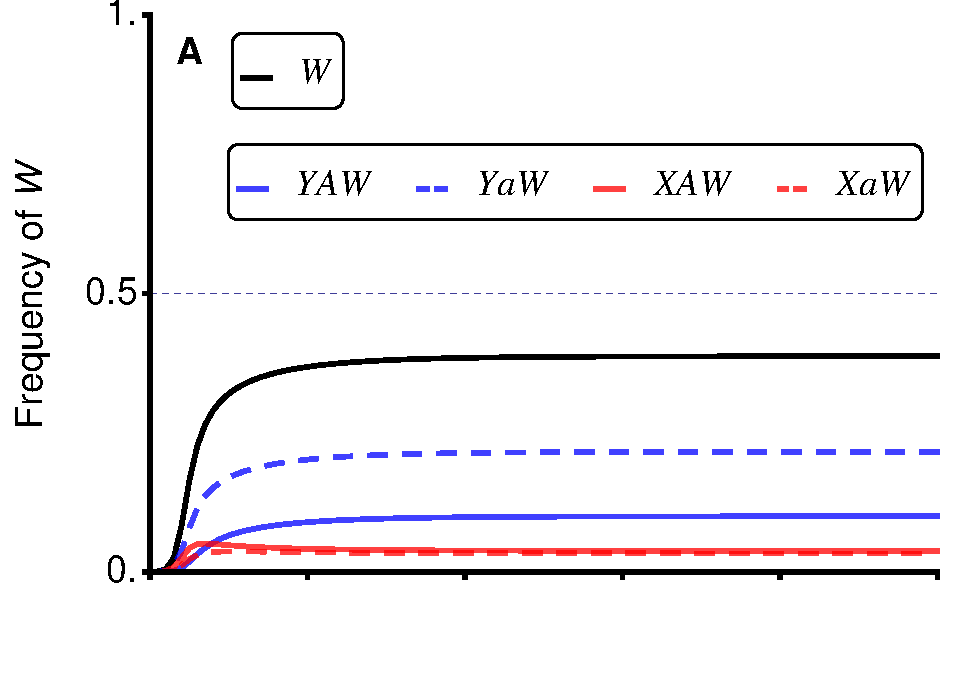
\includegraphics[width=0.5\linewidth]{FreqWHighR}\\
%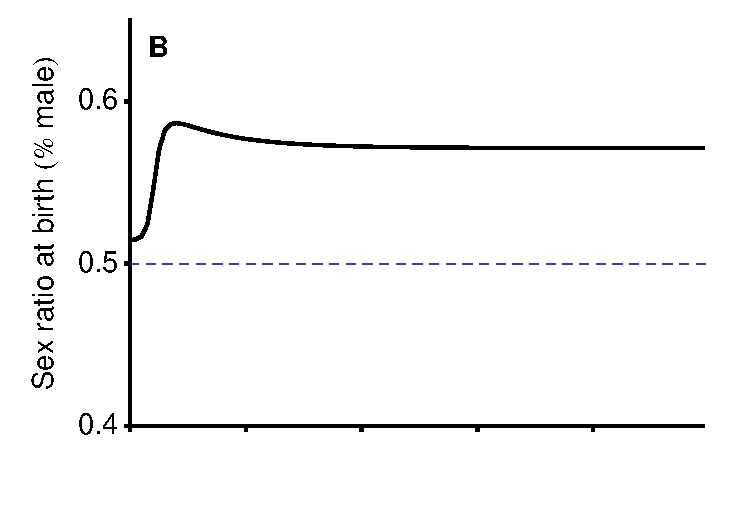
\includegraphics[width=0.5\linewidth]{SexRatioHighR}\\
%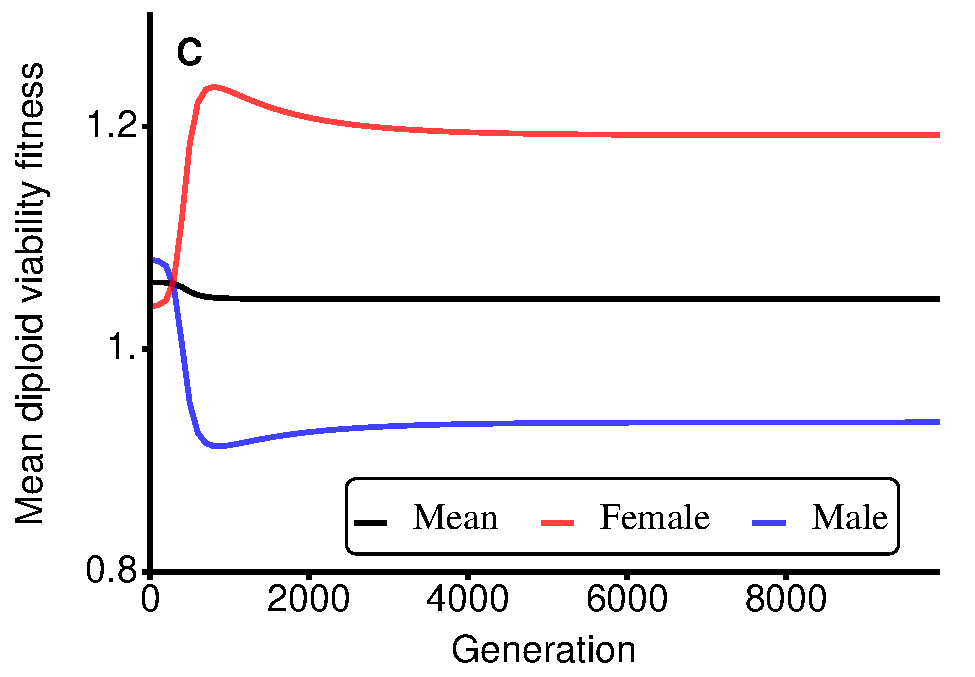
\includegraphics[width=0.5\linewidth]{MeanDipFitHighR}
%\caption{
%Haploid selection allows a completely unlinked neo-$W$ to invade an ancestral $XY$ system (\textbf{A}) despite further biasing the sex ratio (\textbf{B}) and decreasing mean diploid viability fitness (\textbf{C}).
%The neo-$W$ does not fix (although variation at the \textbf{A} locus is maintained, $V_A>0$), resulting in a polymorphic sex-determination system.
%Parameters as in Figure \ref{fig:WinvasionLowR} but with $R=0.5$.
%}
%\label{fig:WinvasionHighR}
%\end{figure}
%%%%%%%%%%%%%%%%%%%%%%%%%%%%%%%%%%%%%%%%%%%%%%%%%%%%%%%%%

%%%%%%%%%%%%%%%%%%%%%%%%%%%%%%%%%%%%%%%%%%%%%%%%%%%%%%%%%
%W invades for all rates of recombination with selected locus
%%%%%%%%%%%%%%%%%%%%%%%%%%%%%%%%%%%%%%%%%%%%%%%%%%%%%%%%%
%\begin{figure}
%\centering
%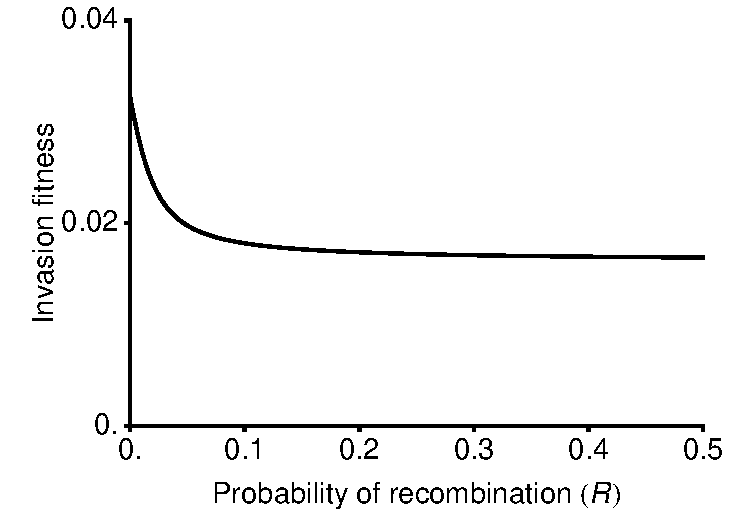
\includegraphics[width=0.5\linewidth]{InvasionVsRecombination}
%\caption{
%A neo-$W$ invades an ancestral $XY$ system with haploid selection regardless of how tightly it is linked to the selected locus. 
%Parameters as in Figure \ref{fig:WinvasionLowR}.
%}
%\label{fig:InvasionVsRecombination}
%\end{figure}
%%%%%%%%%%%%%%%%%%%%%%%%%%%%%%%%%%%%%%%%%%%%%%%%%%%%%%%%%

%%%%%%%%%%%%%%%%%%%%%%%%%%%%%%%%%%%%%%%%%%%%%%%%%%%%%%%%%
%W invasion versus position of selected locus
%%%%%%%%%%%%%%%%%%%%%%%%%%%%%%%%%%%%%%%%%%%%%%%%%%%%%%%%%
%\begin{figure}
%\centering
%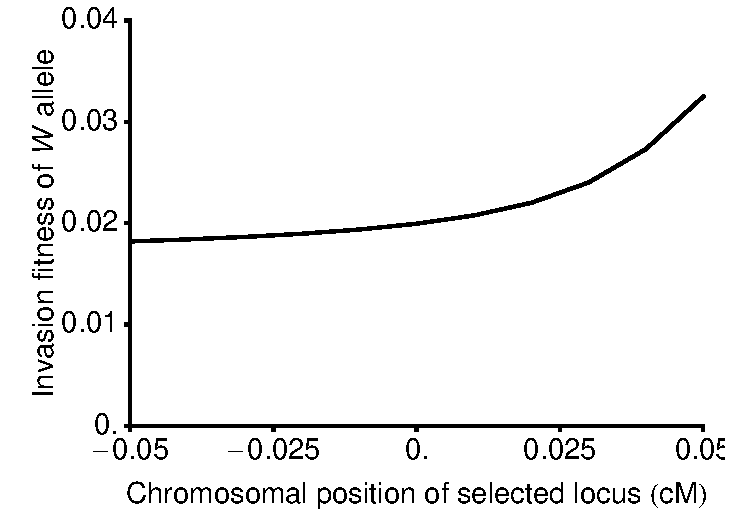
\includegraphics[width=0.5\linewidth]{InvasionVsCentiMorgans}
%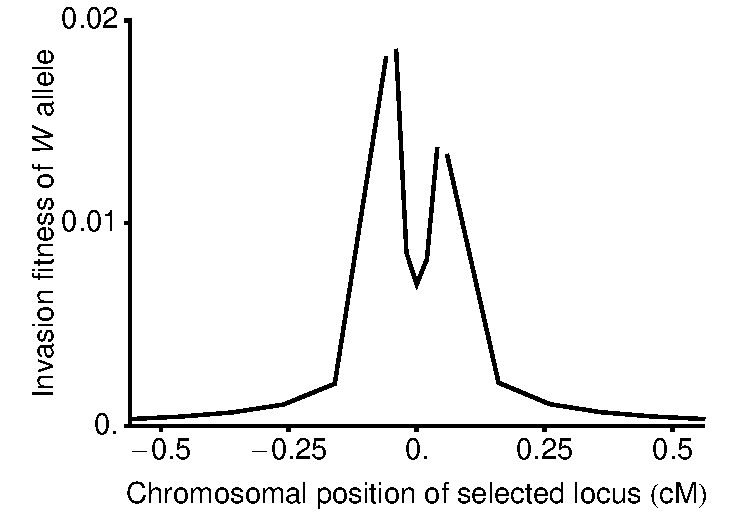
\includegraphics[width=0.5\linewidth]{InvasionVsCentiMorgansAllOrders}
%\caption{
%Haploid selection allows a neo-$W$ to invade an ancestral $XY$ system regardless of how tightly it and the ancestral sex-determining locus are linked to the selected locus. 
%The ancestral sex-determining locus is located at -0.05 and the novel sex-determining locus is located at 0.05 (corresponding to the peaks of invasion fitness), such that the probability of a cross-over between them is $\approx0.1$.
%The x-axis gives the position of the locus under haploid selection.
%We used Haldane's map function \citep[Equation 3 in ][]{Haldane1919} to convert from map distance (centiMorgans) to the probability of a cross-over event. 
%Parameters as in Figure \ref{fig:WinvasionLowR}.
%}
%\label{fig:InvasionVsCentiMorgans}
%\end{figure}
%%%%%%%%%%%%%%%%%%%%%%%%%%%%%%%%%%%%%%%%%%%%%%%%%%%%%%%%%

%%%%%%%%%%%%%%%%%%%%%%%%%%%%%%%%%%%%%%%%%%%%%%%%%%%%%%%%%
%Y invades ZW and fixes (counter example to Kozi explanation)
%%%%%%%%%%%%%%%%%%%%%%%%%%%%%%%%%%%%%%%%%%%%%%%%%%%%%%%%%
%\begin{figure}
%\centering
%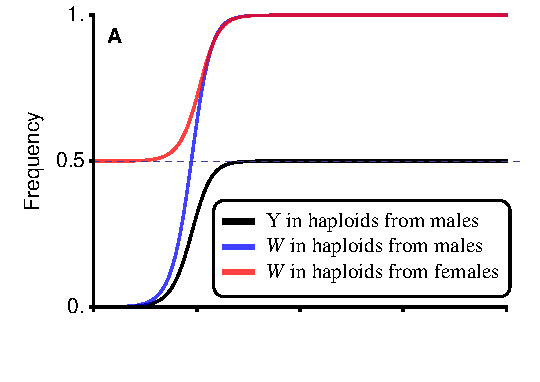
\includegraphics[width=0.5\linewidth]{FreqWCounterKozi}\\
%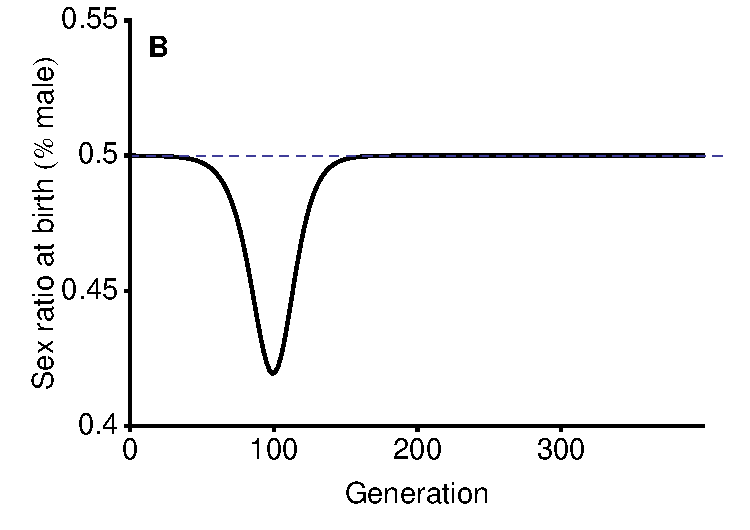
\includegraphics[width=0.5\linewidth]{SexRatioCounterKozi}\\
%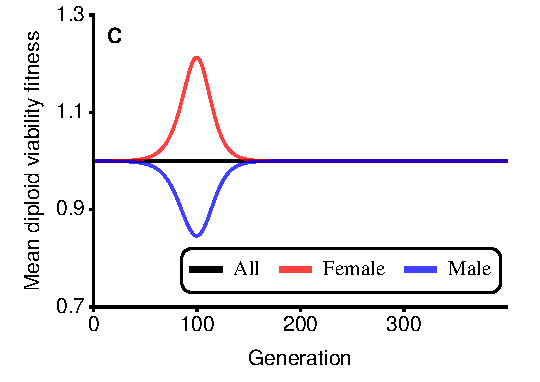
\includegraphics[width=0.5\linewidth]{MeanDipFitCounterKozi}
%\caption{
%Meiotic drive allows a neo-$Y$ to invade an ancestral $ZW$ system and fix (\textbf{A}) despite temporarily biasing the sex ratio (\textbf{B}). %and decreasing mean diploid viability fitness (\textbf{C}).
%Parameters: $k=0$, $s^\female = s^\male = t^\female = t^\male = 0$, $\alpha^\male = 0.4$, $\alpha^\female = 1/2$, $r=0$, $R=0$.
%}
%\label{fig:CounterKozi}
%\end{figure}
%%%%%%%%%%%%%%%%%%%%%%%%%%%%%%%%%%%%%%%%%%%%%%%%%%%%%%%%%

\setcounter{equation}{0}
\renewcommand{\theequation}{S.\arabic{equation}}
\setcounter{figure}{0}
\renewcommand{\thefigure}{S.\arabic{figure}}
\setcounter{table}{0}
\renewcommand{\thetable}{S.\arabic{table}}

%%%%%%%%%%%%%%%%%%%%%%%%%%%%%%%%%%%%%%%%%%%%%%%%%%%%%%%%%
\newpage

\section*{Appendix}

\subsection*{Recursion equations}
\label{app:recurs}

%\textcolor{red}{Should we adjust the subscripts throughout this subsection? Right now we end up re-defining $i$ and $j$ (when switching from haploid to diploid; this might have been my doing!) and then introduce three new subscripts $b$, $c$, and $l$, all of which can be derived from $i$ and $j$. Might be more straightforward to just use $p^\Hermaphrodite_{x_1,x_2,a_1,a_2,m_1,m_2}$ where 1 is maternal and 2 is paternal? We then no longer have to switch indices from haploid to diploid and the connection to other variables is clear: $b=m_1m_2$, $c=x_1x_2$, and $l=a_1a_2$. I guess the downside will be re-writing the recursion equations... which is why I haven't gone ahead and tried this.}

In each generation we census the genotype frequencies in male and female gametes/gametophytes (hereafter, gametes) between meiosis (and any meiotic drive) and gametic competition. 
At this stage we denote the frequencies of X- and Y-bearing gametes from males and females $x_{i}^{\Hermaphrodite}$ and $y_{i}^{\Hermaphrodite}$.
The superscript $\Hermaphrodite \in \{\male,\female\}$ specifies the sex of the diploid that the gamete came from. 
The subscript $i\in\{1,2,3,4\}$ specifies the genotype at the selected locus $\mathbf{A}$ and at the novel sex-determining locus $\mathbf{M}$, where $1=AM$, $2=aM$, $3=Am$, and $4=am$. 
The gamete frequencies from each sex sum to one, $\sum_{i}x_{i}^{\Hermaphrodite}+y_{i}^{\Hermaphrodite}=1$. 

Competition then occurs among gametes of the same sex (e.g., among eggs and among sperm separately) according to the genotype at the \textbf{A} locus ($w_{1}^\Hermaphrodite=w_{3}^\Hermaphrodite=w_{A}^\Hermaphrodite$, $w_{2}^\Hermaphrodite=w_{4}^\Hermaphrodite=w_{a}^\Hermaphrodite$, see Table \ref{tab:fitnesstable}).
The genotype frequencies after gametic competition are $x_{i}^{\Hermaphrodite,s}= w_{i}x_{i}^{\Hermaphrodite}/\bar{w}_{H}^{\Hermaphrodite}$ and $y_{i}^{\Hermaphrodite,s}= w_{i}y_{i}^{\Hermaphrodite}/\bar{w}_{H}^{\Hermaphrodite}$, where $\bar{w}_{H}^{\Hermaphrodite}=\sum_{i} w_{i}x_{i}^{\Hermaphrodite}+w_{i}y_{i}^{\Hermaphrodite}$ is the mean fitness of male ($\Hermaphrodite=\male$) or female ($\Hermaphrodite=\female$) gametes. 

Random mating then occurs between gametes to produce diploid zygotes.
%To shorten notation we now use index $i$ (and $j$) to denote the alleles at both the $\mathbf{A}$ and $\mathbf{M}$ loci and label $MA=1$, $Ma=2$, $mA=3$, and $ma=4$, such that $i,j\in\{1,2,3,4\}$.
The frequencies of XX zygotes are then denoted as $xx_{ij}$, XY zygotes as $xy_{ij}$, and YY zygotes as $yy_{ij}$, where \textbf{A} and \textbf{M} locus genotypes are given by $i,j\in\{1,2,3,4\}$, as above. 
In $XY$ zygotes, the haplotype inherited from an X-bearing gamete is given by $i$ and the haplotype from a Y-bearing gamete is given by $j$. 
In XX and YY zygotes, individuals with diploid genotype $ij$ are equivalent to those with diploid genotype $ji$; for simplicity, we use $xx_{ij}$ and $yy_{ij}$ with $i\neq j$ to denote the average of these frequencies, $xx_{ij}=(x_{i}^{\female,s}x_{j}^{\male,s}+x_{j}^{\female,s}x_{i}^{\male,s})/2$ and $yy_{ij}=(y_{i}^{\female,s}y_{j}^{\male,s}+y_{j}^{\female,s}y_{i}^{\male,s})/2$. 


Denoting the \textbf{M} locus genotype by $b \in \{MM, Mm, mm\}$ and the \textbf{X} locus genotype by $c \in \{XX, XY, YY\}$, zygotes develop as females with probability $k_{bc}$. 
Therefore, the frequencies of XX females are given by $xx_{ij}^{\female}=k_{bc}xx_{ij}$, XY females are given by $xy_{ij}^{\female}=k_{bc}xy_{ij}$, and YY females are given by $yy_{ij}^{\female}=k_{bc}yy_{ij}$. 
Similarly, XX male frequencies are $xx_{ij}^{\male}=(1-k_{bc})xx_{ij}$, XY male frequencies are $xy_{ij}^{\male}=(1-k_{bc})xy_{ij}$, and YY males frequencies are $yy_{ij}^{\male}=(1-k_{bc})yy_{ij}$.
This notation allows both the ancestral and novel sex-determining regions to determine zygotic sex according to an XY system, a ZW system, or an environmental sex-determining system. 
In addition, we can consider any epistatic dominance relationship between the two sex-determining loci. 
Here, we assume that the ancestral sex-determining system (\textbf{X} locus) is XY ($k_{MMXX}=1$ and $k_{MMXY}=k_{MMYY}=0$) or ZW ($k_{MMZZ}=0$ and $k_{MMZW}=k_{MMWW}=1$) and epistatically recessive to a dominant novel sex-determining locus, \textbf{M} ($k_{Mmc}=k_{mmc}=k$). 


Selection among diploids then occurs according to the diploid genotype at the \textbf{A} locus, $l \in \{AA, Aa, aa\}$, for an individual of type $ij$ (see Table \ref{tab:fitnesstable}). 
The diploid frequencies after selection in sex $\Hermaphrodite$ are given by $xx_{ij}^{\Hermaphrodite,s}=w_{l}^{\Hermaphrodite} xx_{ij}/\bar{w}^{\Hermaphrodite}$, $xy_{ij}^{\Hermaphrodite,s}=w_{l}^{\Hermaphrodite} xy_{ij}/\bar{w}^{\Hermaphrodite}$, and $yy_{ij}^{\Hermaphrodite,s}=w_{l}^{\Hermaphrodite} yy_{ij}/\bar{w}^{\Hermaphrodite}$, where $\bar{w}^{\Hermaphrodite}= \sum_{i=1}^{4}\sum_{j=1}^{4}w_{l}^{\Hermaphrodite}xx_{ij}+w_{l}^{\Hermaphrodite}xy_{ij}+w_{l}^{\Hermaphrodite}yy_{ij}$ is the mean fitness of individuals of sex $\Hermaphrodite$. 

Finally, these diploids undergo meiosis to produce the next generation of gametes. 
Recombination and sex-specific meiotic drive occur during meiosis.
%We can also assume that recombination is sex specific and/or affected by the M locus - but generally we don't so I just describe $R=R_{f}=R, r_{MM,d}=r_{Mm,d}=r_{mm,d}=r, \chi_{m}=\chi_{f}=\chi$.
Here, we allow any relative locations for the SDR, \textbf{A}, and \textbf{M} loci by using three parameters to describe the recombination rates between them. 
$R$ is the recombination rate between the \textbf{A} locus and the \textbf{M} locus, $\rho$ is the recombination rate between the \textbf{M} locus and the \textbf{X} locus, and $r$ is the recombination rate between the \textbf{A} locus and the \textbf{X} locus. 
Table \ref{tab:chisubstitutions} shows replacements that can be made for each possible ordering of the loci assuming that there is no cross-over interference.
During meiosis in sex $\Hermaphrodite$, meiotic drive occurs such that, in $Aa$ heterozygotes, a fraction $\alpha^{\Hermaphrodite}$ of gametes produced carry the $A$ allele and $(1-\alpha^\Hermaphrodite)$ carry the $a$ allele. 

\begin{table}[ht]
\centering
\smallskip
\caption{
Substitutions for different loci orders assuming no interference. %and $r,R\in(0,1/2)$.\textcolor{blue}{write all in form of first line? so that 1/2 cases are okay (can't determine chi if R is 1/2 in second line, or if r is 1/2 in third line}
}
\begin{tabular}{l l}
\hline\hline
  Order of loci &   \\ [0.5ex] \hline
  SDR-A-M & $\rho=r(1-R)+R(1-r)$  \\
  SDR-M-A & $r=\rho(1-R)+R(1-\rho)$ \\ %$\rho=(r-R)/(1-2R)$ \\
  A-SDR-M & $R=r(1-\rho)+\rho(1-r)$ \\ %$\rho=(R-r)/(1-2r)$ \\
  \hline \hline
  \label{tab:chisubstitutions}
 \end{tabular}
\end{table}

Among gametes from sex $\Hermaphrodite$, the frequencies of haplotypes (before gametic competition) in the next generation are given by

\begingroup
\allowdisplaybreaks
\begin{subequations}
\begin{align}
%
\begin{split}
x_{1}^{{\Hermaphrodite}'}=&xx_{11}^{\Hermaphrodite,s}+xx_{13}^{\Hermaphrodite,s}/2+(xx_{12}^{\Hermaphrodite,s}+xx_{14}^{\Hermaphrodite,s})\alpha^\Hermaphrodite\\
&-R(xx_{14}^{\Hermaphrodite,s}-xx_{23}^{\Hermaphrodite,s}) \alpha^\Hermaphrodite\\
&+(xy_{11}^{\Hermaphrodite,s}+xy_{13}^{\Hermaphrodite,s})/2+(xy_{12}^{\Hermaphrodite,s}+xy_{14}^{\Hermaphrodite,s})\alpha^\Hermaphrodite\\
&- r(xy_{12}^{\Hermaphrodite,s}-xy_{21}^{\Hermaphrodite,s})\alpha^\Hermaphrodite - \rho(xy_{13}^{\Hermaphrodite,s}-xy_{31}^{\Hermaphrodite,s})/2\\
&+\big{[}-(R+r+\rho)xy_{14}^{\Hermaphrodite,s} +(R+\rho-r)xy_{41}^{\Hermaphrodite,s}\\
&+(R+r-\rho) xy_{23}^{\Hermaphrodite,s}+(R+\rho-r)xy_{32}^{\Hermaphrodite,s}\big{]}\alpha^\Hermaphrodite/2
\end{split}
\\
%
\begin{split}
x_{2}^{{\Hermaphrodite}'}=&xx_{22}^{\Hermaphrodite,s}+xx_{24}^{\Hermaphrodite,s}/2+(xx_{12}^{\Hermaphrodite,s}+xx_{23}^{\Hermaphrodite,s})\alpha^\Hermaphrodite\\
&-R(xx_{23}^{\Hermaphrodite,s}-xx_{14}^{\Hermaphrodite,s}) \alpha^\Hermaphrodite\\
&(xy_{22}^{\Hermaphrodite,s}+xy_{24}^{\Hermaphrodite,s})/2+(xy_{21}^{\Hermaphrodite,s}+xy_{23}^{\Hermaphrodite,s})(1-\alpha^\Hermaphrodite)\\
&- r(xy_{21}^{\Hermaphrodite,s}-xy_{12}^{\Hermaphrodite,s})(1-\alpha^\Hermaphrodite) - \rho(xy_{24}^{\Hermaphrodite,s}-xy_{42}^{\Hermaphrodite,s})/2\\
&+\big{[}-(R+r+\rho)xy_{23}^{\Hermaphrodite,s}+(R+\rho-r)xy_{32}^{\Hermaphrodite,s}\\
&+(R+r-\rho) xy_{14}^{\Hermaphrodite,s}+(R+\rho-r)xy_{41}^{\Hermaphrodite,s}\big{]}(1-\alpha^\Hermaphrodite)/2
\end{split}
\\
%
\begin{split}
x_{3}^{{\Hermaphrodite}'}=&xx_{33}^{\Hermaphrodite,s}+xx_{13}^{\Hermaphrodite,s}/2+(xx_{23}^{\Hermaphrodite,s}+xx_{34}^{\Hermaphrodite,s})\alpha^\Hermaphrodite\\
&-R(xx_{23}^{\Hermaphrodite,s}-xx_{14}^{\Hermaphrodite,s}) \alpha^\Hermaphrodite\\
&(xy_{33}^{\Hermaphrodite,s}+xy_{31}^{\Hermaphrodite,s})/2+(xy_{32}^{\Hermaphrodite,s}+xy_{34}^{\Hermaphrodite,s})\alpha^\Hermaphrodite\\
&- r(xy_{34}^{\Hermaphrodite,s}-xy_{43}^{\Hermaphrodite,s}) \alpha^\Hermaphrodite - \rho(xy_{31}^{\Hermaphrodite,s}-xy_{13}^{\Hermaphrodite,s})/2\\
&+\big{[}-(R+r+\rho)xy_{32}^{\Hermaphrodite,s} +(R+\rho-r)xy_{23}^{\Hermaphrodite,s}\\
&+(R+r-\rho) xy_{41}^{\Hermaphrodite,s}+(R+\rho-r)xy_{14}^{\Hermaphrodite,s}\big{]} \alpha^\Hermaphrodite/2
\end{split}
\\
%
\begin{split}
x_{4}^{{\Hermaphrodite}'}=&xx_{44}^{\Hermaphrodite,s}+xx_{34}^{\Hermaphrodite,s}/2+(xx_{14}^{\Hermaphrodite,s}+xx_{24}^{\Hermaphrodite,s})\alpha^\Hermaphrodite\\
&-R(xx_{14}^{\Hermaphrodite,s}-xx_{23}^{\Hermaphrodite,s}) \alpha^\Hermaphrodite\\
&(xy_{44}^{\Hermaphrodite,s}+xy_{42}^{\Hermaphrodite,s})/2+(xy_{41}^{\Hermaphrodite,s}+xy_{43}^{\Hermaphrodite,s})(1-\alpha^\Hermaphrodite)\\
&- r(xy_{43}^{\Hermaphrodite,s}-xy_{34}^{\Hermaphrodite,s})(1-\alpha^\Hermaphrodite) - \rho(xy_{42}^{\Hermaphrodite,s}-xy_{24}^{\Hermaphrodite,s})/2\\
&+\big{[}-(R+r+\rho)xy_{41}^{\Hermaphrodite,s}+(R+\rho-r)xy_{14}^{\Hermaphrodite,s}\\
&+(R+r-\rho) xy_{32}^{\Hermaphrodite,s}+(R+\rho-r)xy_{23}^{\Hermaphrodite,s}\big{]}(1-\alpha^\Hermaphrodite)/2
\end{split}
\\
\begin{split}
y_{1}^{{\Hermaphrodite}'}=&yy_{11}^{\Hermaphrodite,s}+yy_{13}^{\Hermaphrodite,s}/2+(yy_{12}^{\Hermaphrodite,s}+yy_{14}^{\Hermaphrodite,s})\alpha^\Hermaphrodite\\
&-R(yy_{14}^{\Hermaphrodite,s}-yy_{23}^{\Hermaphrodite,s}) \alpha^\Hermaphrodite\\
&(xy_{11}^{\Hermaphrodite,s}+xy_{31}^{\Hermaphrodite,s})/2+(xy_{21}^{\Hermaphrodite,s}+xy_{41}^{\Hermaphrodite,s})\alpha^\Hermaphrodite\\
&- r(xy_{21}^{\Hermaphrodite,s}-xy_{12}^{\Hermaphrodite,s})\alpha^\Hermaphrodite - \rho(xy_{31}^{\Hermaphrodite,s}-xy_{13}^{\Hermaphrodite,s})/2\\
&+\big{[} - (R+r+\rho)xy_{41}^{\Hermaphrodite,s} + (R+\rho-r)xy_{14}^{\Hermaphrodite,s}\\
& + (R+r-\rho)xy_{32}^{\Hermaphrodite,s} + (R+\rho-r) xy_{23}^{\Hermaphrodite,s}\big{]}\alpha^\Hermaphrodite/2
\end{split}
\\
%
\begin{split}
y_{2}^{{\Hermaphrodite}'}=&yy_{22}^{\Hermaphrodite,s}+yy_{24}^{\Hermaphrodite,s}/2+(yy_{12}^{\Hermaphrodite,s}+yy_{23}^{\Hermaphrodite,s})\alpha^\Hermaphrodite\\
&-R(yy_{23}^{\Hermaphrodite,s}-yy_{14}^{\Hermaphrodite,s}) \alpha^\Hermaphrodite\\
&(xy_{22}^{\Hermaphrodite,s}+xy_{42}^{\Hermaphrodite,s})/2+(xy_{12}^{\Hermaphrodite,s}+xy_{32}^{\Hermaphrodite,s})(1-\alpha^\Hermaphrodite)\\
&- r(xy_{12}^{\Hermaphrodite,s}-xy_{21}^{\Hermaphrodite,s})(1-\alpha^\Hermaphrodite) - \rho(xy_{42}^{\Hermaphrodite,s}-xy_{24}^{\Hermaphrodite,s})/2\\
&+\big{[}-(R+r+\rho)xy_{32}^{\Hermaphrodite,s} +(R+\rho-r) xy_{23}^{\Hermaphrodite,s}\\
&+(R+r-\rho)xy_{41}^{\Hermaphrodite,s}+(R+\rho-r)xy_{14}^{\Hermaphrodite,s}\big{]}(1-\alpha^\Hermaphrodite)/2
\end{split}
\\
%
\begin{split}
y_{3}^{{\Hermaphrodite}'}=&yy_{33}^{\Hermaphrodite,s}+yy_{13}^{\Hermaphrodite,s}/2+(yy_{23}^{\Hermaphrodite,s}+yy_{34}^{\Hermaphrodite,s})\alpha^\Hermaphrodite\\
&-R(yy_{23}^{\Hermaphrodite,s}-yy_{14}^{\Hermaphrodite,s}) \alpha^\Hermaphrodite\\
&(xy_{33}^{\Hermaphrodite,s}+xy_{13}^{\Hermaphrodite,s})/2+(xy_{23}^{\Hermaphrodite,s}+xy_{43}^{\Hermaphrodite,s})\alpha^\Hermaphrodite\\
&- r(xy_{43}^{\Hermaphrodite,s}-xy_{34}^{\Hermaphrodite,s})\alpha^\Hermaphrodite - \rho(xy_{13}^{\Hermaphrodite,s}-xy_{31}^{\Hermaphrodite,s})/2\\
&+\big{[}-(R+r+\rho)xy_{23}^{\Hermaphrodite,s} +(R+\rho-r)xy_{32}^{\Hermaphrodite,s}\\
&+(R+r-\rho) xy_{14}^{\Hermaphrodite,s} + (R+\rho-r) xy_{41}^{\Hermaphrodite,s}\big{]}\alpha^\Hermaphrodite/2
\end{split}
\\
%
\begin{split}
y_{4}^{{\Hermaphrodite}'}=&yy_{44}^{\Hermaphrodite,s}+yy_{34}^{\Hermaphrodite,s}/2+(yy_{14}^{\Hermaphrodite,s}+yy_{24}^{\Hermaphrodite,s})\alpha^\Hermaphrodite\\
&-R(yy_{14}^{\Hermaphrodite,s}-yy_{23}^{\Hermaphrodite,s}) \alpha^\Hermaphrodite\\
&(xy_{44}^{\Hermaphrodite,s}+xy_{24}^{\Hermaphrodite,s})/2+(xy_{14}^{\Hermaphrodite,s}+xy_{34}^{\Hermaphrodite,s})(1-\alpha^\Hermaphrodite)\\
&- r(xy_{34}^{\Hermaphrodite,s}-xy_{43}^{\Hermaphrodite,s})(1-\alpha^\Hermaphrodite) - \rho(xy_{24}^{\Hermaphrodite,s}-xy_{42}^{\Hermaphrodite,s})/2\\
&+\big{[}-(R+r+\rho) xy_{14}^{\Hermaphrodite,s} + (R+\rho-r)xy_{41}^{\Hermaphrodite,s}\\
&+(R+r-\rho) xy_{23}^{\Hermaphrodite,s} + (R+\rho-r) xy_{32}^{\Hermaphrodite,s}\big{]}(1-\alpha^\Hermaphrodite)/2
\end{split}
\end{align}
\label{eq:recursions}
\end{subequations}

\endgroup

\noindent
The full system is therefore described by 16 recurrence equations (three diallelic loci in two sexes, $2^3 \times 2 = 16$). 
However, not all diploid types are produced under certain sex-determination systems. 
For example, with the $M$ allele fixed and an ancestral $XY$ sex-determining system, there are $XX$ males, $XY$ females, or $YY$ females ($x_{3}^\Hermaphrodite=x_{4}^\Hermaphrodite=y_{4}^\Hermaphrodite=y_{3}^\Hermaphrodite=y_{i}^\female=0$). 
%($xx_{11}^{\male}=xx_{12}^{\male}=xx_{22}^\male=xy_{11}^{\female}=xy_{12}^{\female}=xy_{21}^{\female}=xy_{22}^\female=yy_{11}^{\female}=yy_{12}^{\female}=yy_{22}^\female=0$). 
In this case, the system only involves six recursion equations, %because there is only one \textbf{M} locus allele and no Y-bearing female gametes. 
which we assume below to calculate the equilibria. 

%I think this should be moved below because we have some 'results' where we don't assume weak selection but we only have the equilibrium calculated analytically for weak selection. 

\subsection*{Resident equilibria and stability}

In the resident population (allele $M$ fixed), we follow the frequency of $A$ in X-bearing female gametes, $p^\female_X$, and X-bearing male gametes, $p^\male_X$, and Y-bearing male gametes, $p^\male_Y$.
We also track the total frequency of Y among male gametes, $q$, which may deviate from $1/2$ due to meiotic drive in males. 
These four variables determine the frequencies of the six resident gamete types: $x_{1}^{\female}=\hat{p}_X^\female$, $x_{2}^{\female}=1-\hat{p}_X^\female$, $x_{1}^{\male}=(1-q)\hat{p}_X^\male$, $x_{2}^{\male}=(1-q)(1-\hat{p}_X^\male)$, $y_{1}^{\male}=q \hat{p}_Y^\male$, and $y_{2}^{\male}=q(1-\hat{p}_Y^\male)$. 
Mean fitnesses in the resident population are given in table \ref{tab:meanfitnesses}.

Various forms of selection can maintain a polymorphism at the \textbf{A} locus, including sexually antagonistic selection, overdominance, conflicts between diploid selection and selection upon haploid genotypes \citep[ploidally antagonistic selection,][]{Immler:2012tl}, or a combination of these selective regimes. 
\textcolor{blue}{add reference or say "see below"}

\begin{table}[ht]
\centering
\smallskip
\caption{Mean fitnesses and zygotic sex ratio in the resident population ($M$ fixed, XY sex determination). }
\begin{tabular}{l l }
\hline\hline
  Sex \& Life Cycle Stage & Mean Fitness \\ [0.5ex] \hline  \noalign{\vskip 0.5ex}
  female gametes ($\bar{w}_H^\female$) & 
  $p_X^\female w_A^\female + (1-p_X^\female) w_a^\female$ \\ [0.5ex] \hline  \noalign{\vskip 0.5ex}
  male gametes ($\bar{w}_H^\male$) & 
  $\bar{p}^{\male} w_A^\male + (1-\bar{p}^{\male}) w_a^\male$ \\ [0.5ex] \hline  \noalign{\vskip 0.5ex}
  females ($\bar{w}^\female$) & 
  $\begin{array}{l}  (1-\zeta)^{-1} \big[ p_X^\female w_A^\female p_X^\male w_A^\male w_{AA}^\female + \\
  (1 - p_X^\female) w_a^\female p_X^\male w_A^\male w_{Aa}^\female + \\
  p_X^\female w_A^\female (1 - p_X^\male) w_a^\male w_{Aa}^\female + \\
  (1-p_X^\female) w_a^\female (1 - p_X^\male) w_a^\male w_{aa}^\female \big] / \left( \bar{w}_H^\female \bar{w}_H^\male \right)
  \end{array} 
  $ \\ [0.5ex] \noalign{\vskip 0.5ex} \hline  \noalign{\vskip 0.5ex}
  males ($\bar{w}^\male$) & 
  $\begin{array}{l} \zeta^{-1} \big[ p_X^\female w_A^\female  p_Y^\male w_A^\male w_{AA}^\male + \\
  (1 - p_X^\female) w_a^\female  p_Y^\male w_A^\male w_{Aa}^\male + \\
  p_X^\female w_A^\female  (1 - p_Y^\male) w_a^\male w_{Aa}^\male + \\
  (1-p_X^\female) w_a^\female  (1 - p_Y^\male) w_a^\male w_{aa}^\male \big] / \left( \bar{w}_H^\female \bar{w}_H^\male \right) 
  \end{array}
  $ \\ [0.5ex] \noalign{\vskip 0.5ex} \hline  \noalign{\vskip 0.5ex}
  fraction zygotes male ($\zeta$) & $q \left[ p_Y^\male w_A^\male+(1-p_Y^\male)w_a^\male\right] / \bar{w}_H^\male $
   \\ [0.5ex]  \noalign{\vskip 0.5ex}
  \hline \hline
  \label{tab:meanfitnesses}
 \end{tabular}
\end{table}

In particular special cases, e.g., no sex-differences in selection or meiotic drive ($s^\male=s^\female$, $h^\male=h^\female$, and $\alpha^\male=\alpha^\female=1/2$), the equilibrium allele frequency and stability can be calculated analytically without assuming anything about the relative strengths of selection and recombination. 
However, here, we focus on two regimes (tight linkage and weak selection) in order to make fewer assumptions about fitnesses. 

\subsubsection*{Recombination weak relative to selection (tight linkage between \textbf{A} and \textbf{X})}

We first calculate the equilibrium frequency of the Y and $A$ alleles in the ancestral population when the recombination rate between the \textbf{X} and \textbf{A} loci is small ($r$ of order $\epsilon$). 
Selection at the \textbf{A} locus will not affect evolution at the novel sex-determining locus, \textbf{M}, if one allele is fixed on all backgrounds. 
We therefore focus on the five equilibria that maintain both $A$ and $a$ alleles, four of which are given to leading order by:

\begin{subequations}\label{eq:tightequil}
\begin{align}
(A)\ \ \ &\hat{p}_{Y}^{\male}=0,
\ \hat{q}=\frac{1}{2}\left(1 - \alpha_\Delta^\male \frac{ w_{Aa}^{\male} \phi}{w_{Aa}^{\male} \phi+ w_{aa}^{\male} \psi}\right),\\
&\hat{p}_{X}^{\female}=\frac{w_{a}^{\female} \phi}{w_{a}^{\female} \phi+ w_{A}^{\female} \psi},
\ \hat{p}_{X}^{\male}=\frac{(1+\alpha_\Delta^\male)w_{Aa}^{\male} \phi}{(1+\alpha_\Delta^\male)w_{Aa}^{\male} \phi +w_{aa}^{\male} \psi} \nonumber \\
(A')\ \ \ &\hat{p}_{Y}^{\male}=1,
\ \hat{q}=\frac{1}{2}\left(1 + \alpha_\Delta^\male \frac{w_{Aa}^{\male} \phi'}{w_{Aa}^{\male} \phi' + w_{AA}^{\male} \psi'}\right),\\
&\hat{p}_{X}^{\female}=1-\frac{w_{A}^{\female} \phi'}{w_{A}^{\female} \phi'+ w_{a}^{\female} \psi'},
\ \hat{p}_{X}^{\male}=1-\frac{(1-\alpha_\Delta^\male)w_{Aa}^{\male} \phi'}{(1-\alpha_\Delta^\male)w_{Aa}^{\male} \phi'+w_{AA}^{\male} \psi'} \nonumber \\
(B)\ \ \ &\hat{p}_{Y}^{\male}=0,\ \hat{p}_{X}^{\female}=1,\ \hat{p}_{X}^{\male}=1, \ \hat{q}=(1 -\alpha^\male_\Delta)/2\\
(B')\ \ \ &\hat{p}_{Y}^{\male}=1,\ \hat{p}_{X}^{\female}=0,\ \hat{p}_{X}^{\male}=0, \ \hat{q}=(1+\alpha^\male_\Delta)/2
\end{align}
\end{subequations}
\begin{equation*}
\begin{split}
\phi=&(1+\alpha^\female_\Delta) w_{A}^{\female} w_{Aa}^{\female} \left[ w_{a}^{\male} w_{aa}^{\male} + (1+\alpha_\Delta^\male) w_{A}^{\male} w_{Aa}^{\male} \right]/2 - w_{a}^{\male} w_{a}^{\female} w_{aa}^{\male} w_{aa}^{\female} \\
\psi=&(1-\alpha^\female_\Delta) w_{a}^{\female} w_{Aa}^{\female} \left[ w_{a}^{\male} w_{aa}^{\male} + (1+\alpha_\Delta^\male) w_{A}^{\male} w_{Aa}^{\male}\right]/2 - (1+\alpha_\Delta^\male) w_{A}^{\male} w_{A}^{\female} w_{Aa}^{\male} w_{AA}^{\female}\\
\phi'=&(1-\alpha^\female_\Delta) w_{a}^{\female} w_{Aa}^{\female} \left[ w_{A}^{\male} w_{AA}^{\male} + (1-\alpha_\Delta^\male) w_{a}^{\male} w_{Aa}^{\male} \right]/2 - w_{A}^{\male} w_{A}^{\female} w_{AA}^{\male} w_{AA}^{\female}\\
\psi'=&(1+\alpha^\female_\Delta) w_{A}^{\female} w_{Aa}^{\female} \left[ w_{A}^{\male} w_{AA}^{\male} + (1-\alpha_\Delta^\male) w_{a}^{\male} w_{Aa}^{\male} \right]/2 - (1-\alpha_\Delta^\male) w_{a}^{\male} w_{a}^{\female} w_{Aa}^{\male} w_{aa}^{\female}
\end{split}
\end{equation*}

\noindent
A fifth equilibrium $(C)$ also exists where $A$ is present at an intermediate frequency on the Y chromosome ($0<\hat{p}_{Y}^{\male}<1$). 
However, equilibrium $(C)$ is never locally stable when $r \approx 0$ and is therefore not considered further.
Thus, the Y can either be fixed for the $a$ allele (equilibria $A$ and $B$) or the $A$ allele (equilibria $A'$ and $B'$).
The X chromosome can then either be polymorphic (equilibria $A$ and $A'$) or fixed for the alternative allele (equilibria $B$ and $B'$).
Since equilibria $(A)$ and $(B)$ are equivalent to equilibria $(A')$ and $(B')$ with the labelling of $A$ and $a$ alleles interchanged, we discuss only equilibria $(A)$ and $(B)$, in which the Y is fixed for the $a$ allele. 
If there is no haploid selection ($\alpha^{\Hermaphrodite}_\Delta=0$, $w_{A}^{\Hermaphrodite}=w_{a}^{\Hermaphrodite}=1$), these equilibria are equivalent to those found by \cite{Lloyd1977} and \cite{Otto2014}.

We next calculate when $(A)$ and $(B)$ are locally stable for $r=0$. 
According to the `small parameter theory' \citep{Karlin:1972ab,Karlin:1972dq}, these stability properties are unaffected by small amounts of recombination between the SDR and \textbf{A} locus, although equilibrium frequencies may be slightly altered. 
For the $a$ allele to be stably fixed on the Y we need $\bar{w}_{Ya}^{\male} > \bar{w}_{YA}^{\male}$ where $\bar{w}_{Ya}^{\male} = w_{a}^{\male} \big[\hat{p}_X^\female(1-\alpha^\male_\Delta) w_{A}^{\female} w_{Aa}^{\male} + (1-\hat{p}_X^\female)w_{a}^{\female} w_{aa}^{\male} \big]$ and $\bar{w}_{YA}^{\male} = w_{A}^{\male} \big[ \hat{p}_X^\female w_{A}^{\female} w_{AA}^{\male} + (1-\hat{p}_X^\female)(1+\alpha^\male_\Delta) w_{a}^{\female} w_{Aa}^{\male} \big]$. 
That is, Y-$a$ haplotypes must have higher fitness than Y-$A$ haplotypes.  
Substituting in $\hat{p}_X^\female$ from equation \eqref{eq:tightequil}, fixation of the $a$ allele on the Y requires that $\gamma_{i}>0$ where $\gamma_{(A)}=w_{a}^{\male} \big[ (1-\alpha^\male_\Delta) w_{Aa}^{\male} \phi + w_{aa}^{\male} \psi \big]-w_{A}^{\male} \big[ w_{AA}^{\male} \phi + (1 + \alpha^{\male}_\Delta)w_{Aa}^{\male} \psi \big]$ for equilibrium $(A)$ and $\gamma_{(B)}=(1-\alpha^{\male}_\Delta)w_{a}^{\male}w_{Aa}^{\male}-w_{A}^{\male}w_{AA}^{\male}$ for equilibrium $(B)$.
Stability of a polymorphism on the X chromosome (equilibrium $A$) further requires that $\phi >0$ and $\psi >0$. 
Fixation of the $a$ allele on the X (equilibrium $B$) can be stable only if equilibrium $(A)$ is not, as it requires $\psi<0$. %and $2w_{A}^{\female}w_{AA}^{\female}>(1-\alpha_\Delta^{\female})w_{a}^{\female}w_{Aa}^{\female}$ or just $4w_{A}^{\female}w_{AA}^{\female}<(1-\alpha_\Delta^{\female})w_{a}^{\female}w_{Aa}^{\female}$ (which also prevents $\psi>0$). 

%\textcolor{red}{check last condition and the stability condition below are correct}
%\textcolor{blue}{The last condition looks good to me, although in your Turnover-norec-MFS.nb you look at YA fixed, so you have to flip everything (so I made Turnover-norec-MFS-MMO.nb to do this).
%The one issue I can find here is that you can also prevent $\lambda>1$ when the slope and intercept of the quadratic at $\lambda=1$ are negative (you only looked at both being positive). In this case we need $4w_{A}^{\female}w_{AA}^{\female}<(1-\alpha_\Delta^{\female})w_{a}^{\female}w_{Aa}^{\female}$, which also prevents $\psi>0$.
%I've added this in.
%It could also be the case that the slope and intercept are the same sign but the roots are imaginary - but this is never the case here.
%Stability condition below looks good to me (from matt version of turnoverSOM-MIKE.nb).}

\subsubsection*{Selection weak relative to recombination (weak selection)}

Here, we assume that selection and meiotic drive are weak relative to recombination ($s^\Hermaphrodite$, $t^\Hermaphrodite$, $\alpha_{\Delta}^\Hermaphrodite$ of order $\epsilon$). 
The maintenance of a polymorphism at the \textbf{A} locus then requires that

\begin{equation}
\begin{split}
0&< - \left[(1-h^\female)s^\female +(1-h^\male) s^\male + t^\female +t^\male + \alpha_{\Delta}^\female+\alpha_{\Delta}^\male\right]\\
%
\text{and }\quad 0&<h^\female s^\female +h^\male s^\male + t^\female +t^\male + \alpha_{\Delta}^\female+\alpha_{\Delta}^\male.
\end{split}
\end{equation}

\noindent
which indicates that a polymorphism can be maintained by various selective regimes. 

Given that a polymorphism is maintained at the \textbf{A} locus by weak selection, the frequencies of $A$ in each type of gamete are the same ($\hat{p}^\female_X=\hat{p}^\male_X=\hat{p}^\male_Y=\bar{p}$) and given, to leading order, by 

\begin{equation}
\bar{p}=\frac{h^\female s^\female + h^\male s^\male +t^\female+t^\male+\alpha_{\Delta}^\female+\alpha_{\Delta}^\male}
{(2h^\female-1)s^\female+(2h^\male-1)s^\male}
+O(\epsilon)
.
\label{eq:pAve}
\end{equation}

\noindent
Differences in frequency between gamete types are of $O(\epsilon)$:

\begin{equation}
\begin{split}
\hat{p}^\male_X-\hat{p}^\female_X&=V_{A}\big{(}D^\male - D^\female +\alpha_{\Delta}^\male-\alpha_{\Delta}^\female \big{)}
+O(\epsilon^2)\\
%
\hat{p}^\male_Y-\hat{p}^\female_X&=V_{A}\left[D^\male - D^\female+\alpha_{\Delta}^\male-\alpha_{\Delta}^\female+(1-2r)(t^\male-t^\female)\right]/2r
+O(\epsilon^2)\\
%
\hat{p}^\male_Y-\hat{p}^\male_X&=V_{A}\left(D^\male - D^\female+\alpha_{\Delta}^\male-\alpha_{\Delta}^\female+t^\male-t^\female\right)(1-2r)/2r
+O(\epsilon^2)
\end{split}
\label{eq:freq_diffs}
\end{equation}

\noindent
where $V_{A}=\bar{p}(1-\bar{p})$ is the variance in the frequency of $A$ and $D^\Hermaphrodite=\big{[} \bar{p}s^\Hermaphrodite+(1-\bar{p})h^\Hermaphrodite s^\Hermaphrodite\big{]} -\big{[} \bar{p}h^\Hermaphrodite s^\Hermaphrodite+(1-\bar{p}) \big{]}$ corresponds to the difference in fitness between $A$ and $a$ alleles in diploids of sex $\Hermaphrodite \in \{\female,\male\}$ ($\bar{p}$ is the leading-order probability of mating with an $A$-bearing gamete from the opposite sex). 
The frequency of Y among male gametes depends upon the difference in the frequency of the $A$ allele between X- and Y-bearing male gametes and the strength of meiotic drive in favour of the $A$ allele in males, $q=1/2+\alpha_{\Delta}^\male(\hat{p}^\male_Y-\hat{p}^\male_X)/2+O(\epsilon^3)$.
Without gametic competition or drive ($\alpha_{\Delta}^\Hermaphrodite=t^\Hermaphrodite=0$) our results reduce to those of \citet{vanDoorn:2007eu}.

% the differences in the frequencies of $A$ in each type of gamete are small, as is the bias in the sex-determining factor from the heterogametic sex, and we can solve for the mean frequency of $A$ across all types ($p_A$), the difference in the frequencies of $A$ between two of the three types, and the bias in the frequency of the sex-determining factor, to first order in selection.
%Linear stability analysis can then be used to determine the stability of this equilibrium.
%Without haploid selection or meiotic drive our results reduce to those of \cite{vanDoorn:2007eu}. %when $k=0$ (neo-$Y$ invading a $ZW$ system) or when $k=1$ (neo-$W$ invading an $XY$ system) (\textcolor{red}{CHECK}).
%However, with haploid selection or meiotic drive a stable polymorphism at locus \textbf{A} no longer requires sexually antagonistic selection. %, as it can also be achieved by ploidally-antagonistic selection.

\subsection*{Invasion conditions}

%Here, we determine whether a rare neo-Y or neo-W allele spreads when rare, which occurs when $\lambda > 1$.
%We begin with the general result and then give explicit solutions under tight linkage and weak selection.
 
%If the average change in frequency of the two haplotypes that carry the $m$ allele ($Am$ and $am$) is positive, invasion will always occur (i.e., if $\left\{(\lambda_{mA}-1)+ (\lambda_{ma}-1) \right\}/2 > 0$ then $\lambda > 1$, see table \ref{tab:haplotype_growth} for $\lambda_{mi}$). 
%If neither haplotype increases in frequency ($\lambda_{mA}, \lambda_{ma} < 1$), the $m$ allele will not invade. 
%Otherwise, the new sex-determining allele increases in frequency on one \textbf{A} background and declines on the other, and invasion requires
%\begin{equation}\label{eq:neoYR}
%R \left[ 
%\frac{p^\female_X w^\female_A w^\male_a (1-\alpha^\male)}{ \bar{w}^\female_H \bar{w}^\male_H (\lambda_{mA}-1)} + 
%p^\female_X \frac{w^\female_A}{\bar{w}^\female_H} \frac{w^\male_a(1-\alpha^\male)}{\bar{w}^\male_H} \frac{1}{\lambda_{mA}-1} + 
%\frac{(1 - p^\female_X) w^\female_a w^\male_A \alpha^\male}{ \bar{w}^\female_H \bar{w}^\male_H (\lambda_{ma}-1)} 
%\right] 
%\frac{w^\male_{Aa}}{q\bar{w}^\male} < 1,
%\end{equation}

%\noindent
%for the neo-$Y$, and 

%\noindent
%\begin{equation}\label{eq:neoWR}
%R \left[ 
%\frac{\bar{p}^\male w^\male_A w^\female_a (1-\alpha^\female)}{ \bar{w}^\male_H \bar{w}^\female_H (\lambda_{mA}-1)} + 
%\frac{(1 - \bar{p}^\male) w^\male_a w^\female_A \alpha^\female}{ \bar{w}^\male_H \bar{w}^\female_H (\lambda_{ma}-1)} 
%\right] 
%\frac{w^\female_{Aa}}{(1-q)\bar{w}^\female} < 1,
%\end{equation}

%\noindent
%for the neo-$W$. 

%Equations \eqref{eq:neoYR} and \eqref{eq:neoWR} show that the new sex-determining allele, $m$, is expected to invade for any probability of recombination between loci \textbf{A} and \textbf{M}, $R$, when the net flow of recombinants is from the less fit (smaller $\lambda_{mi}$) to the more fit \textbf{A} background (making the terms inside the square brackets in Equations \ref{eq:neoYR} and \ref{eq:neoWR} negative). %\textcolor{red}{Q: is it definitely possible to have negative square brackets for a equilibria maintained by selection?}
%Assuming $g_A^* > 0$ and $g_a^* < 0$ without loss of generality, this is $-(1 - p^\female_X) w_{m,A} g_a^* < p^\female_X w_{m,a} g_A^*$.
%When the net flow of recombinants is from the more fit to the less fit haplotype, the new sex-determining allele can still invade when the rate of recombination between it and the selected locus is small enough. %\textcolor{red}{Q:Is it the case that sometimes the square brackets are positive and invasion occurs for $r_{AM}=1/2$? In which case it might be better to have slightly different phrasing here.}
%Equations \eqref{eq:neoYR} and \eqref{eq:neoWR} show that the new sex-determining allele, $m$, is expected to invade for any probability of recombination between loci \textbf{A} and \textbf{M}, $R$, when the net flow of recombinants is from the less fit (smaller $\lambda_{mi}$) to the more fit \textbf{A} background (making the terms inside the square brackets in Equations \ref{eq:neoYR} and \ref{eq:neoWR} negative).
%When the net flow of recombinants is from the more fit to the less fit haplotype, the new sex-determining allele can still invade when the rate of recombination between it and the selected locus is small enough. 
%To better understand when these scenarios are possible we next use knowledge of the equilibria and their stability under tight linkage and weak selection.

\textcolor{red}{Cover the other parts of the characteristic polynomial here.}
\textcolor{blue}{Waiting for Sally's proof!}

A rare neo-Y or neo-W will spread from a given ancestral equilibrium when the leading eigenvalue, $\lambda$, of the Jacobian matrix derived from the eight mutant recursion equations (given by \ref{eq:recursions}c,d,g,h), evaluated at the ancestral equilibrium, is greater than one.
However, because a neo-Y (neo-W) is always in males (females) and is epistatically dominant to the ancestral sex-determining locus, we need only two recursion equations (e.g., tracking the change in the frequency of neo-Y-$A$ and neo-Y-$a$ gametes from males) and thus the leading eigenvalue is the largest solution to a quadratic characteristic polynomial $\lambda^2 + b\lambda + c = 0$ as described in the text (Table \ref{tab:haplotype_growth}).
%It can be shown (see supplementary Mathematica file) that the coefficients are $b= - (\lambda_{mA} + \lambda_{ma})+(\chi_{mA} + \chi_{ma})$ and $c = (\lambda_{mA}-\chi_{mA}) (\lambda_{ma}-\chi_{ma}) -\chi_{mA} \chi_{ma}$, where $\lambda_{mi}$ is the multiplicative growth rate of the frequency of mutants on background $i\in\{A,a\}$, without accounting for loss due to recombination, and $\chi_{mi}$ is the rate at which mutants on background $i\in\{A,a\}$ recombine onto the other \textbf{A} locus background in heterozygotes.
%The leading eigenvalue is then greater than one whenever $\lambda_{mA}>1$ and $\lambda_{ma}>1$, less than one whenever $\lambda_{mA}<1$ and $\lambda_{ma}<1$, and greater than one whenever  $\lambda_{mA}>1$ or $\lambda_{ma}>1$ and $\chi_{ma} (\lambda_{mA}-1) + \chi_{mA} (\lambda_{ma}-1) > 0$.

The general conditions for the invasion of a neo-sex-determining allele are given in the main text, in terms of the growth rates of the mutant haplotypes in the absence of recombination ($\lambda_{mi}$) and the rate that recombination destroys them ($\chi_{mi}$).
For tight linkage between the ancestral sex-determining locus and the selected locus we can calculate these terms explicitly (see below).
For weak selection we can take a Taylor series of the leading eigenvalue. 
The leading eigenvalue, $\lambda$, for any $k$, is given up to order $\epsilon^2$ by equation \eqref{eq:lambda_ESD_k}.

\subsubsection*{Tight linkage between \textbf{A} and \textbf{X} (recombination weak relative to selection)}

Here, we explore the conditions under which a neo-W invades an XY system assuming that the \textbf{A} locus is initially in tight linkage with the ancestral sex-determining region ($r \approx 0$). 
We disregard neo-Y mutations, which never spread given that the ancestral population is at a stable equilibrium (see supplementary \textit{Mathematica} notebook for proof). 

Starting with the simpler equilibrium $(B)$, the terms of the characteristic polynomial are

\begin{subequations}\label{Binvasion}
\begin{align}
\lambda_{mA}&= \left[w_{A}^\male (1+\alpha^\male_\Delta) \right]^{-1}
\frac{w_{A}^\female }{w_{A}^\female}
\frac{\left[ w_{A}^\male (1+\alpha^\male_\Delta) w_{AA}^\female + 
w_{a}^\male (1-\alpha^\male_\Delta) w_{Aa}^\female (1+\alpha^\female_\Delta) \right]}
{ 2w_{AA}^\female } \\
\lambda_{ma}&= \left[w_{A}^\male (1+\alpha^\male_\Delta) \right]^{-1}
\frac{w_{a}^\female}{w_{A}^\female}
\frac{\left[  w_{A}^\male (1+\alpha^\male_\Delta) w_{Aa}^\female (1-\alpha^\female_\Delta)+
w_{a}^\male (1-\alpha^\male_\Delta) w_{aa}^\female \right]}
{ 2w_{AA}^\female } \\
\chi_{mA}&= \frac{1}{2} \left[w_{A}^\male (1+\alpha^\male_\Delta) \right]^{-1}
\frac{w_{A}^\female }{w_{A}^\female}
 \frac{\left[  w_{a}^\male (1-\alpha^\male_\Delta) w_{Aa}^\female (1 + \alpha^\female_\Delta) \right]}
{ w_{AA}^\female } \frac{R}{2}\\
\chi_{ma}&= \frac{1}{2} \left[w_{A}^\male (1+\alpha^\male_\Delta) \right]^{-1}
\frac{w_{a}^\female}{w_{A}^\female}
 \frac{\left[  w_{A}^\male (1+\alpha^\male_\Delta) w_{Aa}^\female (1-\alpha^\female_\Delta) \right]}
{  w_{AA}^\female} \frac{R}{2}
\end{align}
\end{subequations}

%\noindent
%In this case, the zygotic sex ratio ($\zeta$) is given by the difference in haploid selection in males on $a$ (fixed on the Y) and $A$ (fixed on the X) alleles, i.e., there are more males than females if $\zeta = \alpha^\male w_A^\male / [(1-\alpha^\male)w_a^\male + \alpha^\male w_A^\male]<1/2$. %$\alpha^\male<1/2$ and/or $w_{a}^\male>w_{A}^\male$. 
%Populations with haploid selection for $a$ in males have a male biased zygotic sex ratio are thus more permissive to invasion by a neo-W ($\lambda_{mA}$ and $\lambda_{ma}$ larger).
%%In addition, the spread of neo-W alleles depends on the fitness of female diploids after mating with an X-$A$ or Y-$a$ male gamete, relative to the fitness of females in the population (all have genotype $AA$ and fitness $w_{AA}^\female$ at this equilibrium). 
%Haploid selection in males has a second effect; the spread rate of neo-W haplotypes is determined by their fitness in diploid females, which depends on their diploid genotype and thus on the male gamete they pair with. 
%Zygotes carrying dominant neo-W alleles will develop as females regardless of their genotype at the XY locus. 
%Therefore, neo-W females result from matings with either X-$A$ or Y-$a$ male gametes. 
%The relative proportion of these male gametes is determined by haploid selection in males; mating with a Y-$a$ male gamete is more likely if the $a$ allele is favoured during male gamete production or competition ($\zeta<1/2$). 
%Thus, neo-W females experience different diploid selection than XX females, and the extent of this difference depends on haploid selection in males.
%Furthermore, haploid selection in females can directly select upon neo-W-$A$ or neo-W-$a$ haplotypes. 
%A neo-W-$A$ female gamete has the same fitness during haploid competition as resident $A$-bearing female gametes. 
%On the other hand, neo-W-$a$ female gametes can be favoured or disfavoured during female haploid competition (favoured if $w_{a}^\female>w_{A}^\female$). 
%Meiotic drive in females ($\alpha^\female$) similarly affects the fitness of these neo-W haplotypes, except that it impacts both haplotypes as meiotic drive only occurs in heterozygotes and therefore does not occur in resident XX females (who are always homozygote $AA$). 

Haploid selection impacts the spread of neo-W haplotypes in three ways.
Firstly, the zygotic sex ratio becomes male biased, $\zeta>1/2$, when the $a$ allele (which is fixed on the Y) is favoured during competition among male gametes or by meiotic drive in males.
Specifically, at equilibrium $(B)$, the fraction female is $1 - \zeta = w_A^\male (1+\alpha^\male_\Delta) / (2\bar{w}_{H}^\male)$ where $2\bar{w}_{H}^\male= \big[w_a^\male (1-\alpha^\male_\Delta) +  w_A^\male (1+\alpha^\male_\Delta) \big]$ has been canceled out in equations \eqref{Binvasion} to leave the term $\left[w_{A}^\male (1+\alpha^\male_\Delta) \right]^{-1}$. 
Male biased sex ratios facilitate the spread of a neo-W because neo-W alleles cause the zygotes that carry them to develop as the rarer, female, sex. 

Secondly, haploid selection in females selects on neo-W haplotypes directly.
At equilibrium $(B)$, the fitness of female gametes under the ancestral sex-determining system is $w_{A}^\female$ such that the relative fitnesses of neo-W-$A$ and neo-W-$a$ haplotypes during female gametic competition are $w_{A}^\female/w_{A}^\female$ and $w_{a}^\female/w_{A}^\female$ (see terms in equation \ref{Binvasion}). 
Meiotic drive in females will also change the proportion of gametes that carry the $A$ versus $a$ alleles, which will be produced by heterozygous females in proportions $(1+\alpha_{\Delta}^\female)/2$ and $(1-\alpha_{\Delta}^\female)/2$, respectively. 
These terms are only associated with heterozygous females, i.e., they are found alongside $w_{Aa}^\female$.

Thirdly, haploid selection in males affects the diploid genotypes of females by altering the allele frequencies in the male gametes that female gametes pair with.
At equlibrium $(B)$, neo-W female gametes will mate with X-$A$ male gametes with probability $ w_A^\male (1+\alpha^\male_\Delta) / (2\bar{w}_{H}^\male)$ and Y-$a$ male gametes with probability $w_a^\male (1-\alpha^\male_\Delta) / (2\bar{w}_{H}^\male)$, where the $2\bar{w}_{H}^\male$ terms have been canceled in equation \eqref{Binvasion} (as mentioned above). 
Thus, for example, neo-W-$A$ haplotypes are found in $AA$ female diploids with probability $ w_A^\male (1+\alpha^\male_\Delta)/ (2\bar{w}_{H}^\male)$ (first term in square brackets in the numerator of equation \ref{Binvasion}a) and in $Aa$ female diploids with probability $w_a^\male (1-\alpha^\male_\Delta) / (2\bar{w}_{H}^\male)$ (see equation \ref{Binvasion}c and the second term in square brackets in the numerator of equation \ref{Binvasion}a).

%For instance, because an epistatically dominant neo-W always causes its carrier to become female, it creates females who carry either Y-$a$ or X-$A$ genotypes from their father.
%Thus, because when there is a polymorphism the X carries some non-zero frequency of $A$, haploid selection in males impacts the diploid genotypes of females (e.g., creating more $Aa$ females when drive in males favours Y-$a$).
%How this affects the spread of the neo-W then depends on diploid and haploid selection in females.

The other terms in equations \eqref{Binvasion} are more easily interpreted if we assume that there is no haploid selection in either sex, in which case $\lambda_{mA}>1$ when $w_{Aa}^\female>w_{AA}^\female$ and $\lambda_{ma}>1$ when $(w_{Aa}^\female+w_{aa}^\female)/2>w_{AA}^\female$.
These conditions cannot be met under purely sexually-antagonistic selection, where $A$ is directionally favoured in females ($w_{AA}^\female>w_{Aa}^\female>w_{aa}^\female$) and $a$ is directionally favoured in males ($w_{AA}^\male>w_{Aa}^\male>w_{aa}^\male$).  
Essentially, the X is then already as specialized as possible for the female beneficial allele ($A$ is fixed on the X), and the neo-W often makes daughters with the Y-$a$ haplotype, increasing the flow of $a$ alleles into females, which reduces the fitness of those females.  

If selection doesn't uniformly favour $A$ in females, however, neo-W-$A$ haplotypes and/or neo-W-$a$ haplotypes can spread ($\lambda_{mA}>1$ and/or $\lambda_{ma}>1$) at this equilibrium.
%If $\lambda_{mA}>1$ (requiring $w_{Aa}^\female>w_{AA}^\female$), the implication is that the neo-W can spread alongside the $A$ allele, despite the fact that the neo-W sometimes brings $Y-a$ haplotypes into females, because $a$ is favoured by selection in females despite $A$ being fixed on the X.
A neo-W can spread alongside the $A$ allele ($\lambda_{mA}>1$), despite the fact that a neo-W brings Y-$a$ haplotypes into females, when $w_{Aa}^\female>w_{AA}^\female$, as stated above.
In this case the $a$ allele is favoured by selection in females despite $A$ being fixed on the X.
For this equilibrium to be stable (i.e.,  to keep $A$ fixed on the X), X-$a$ cannot be overly favoured in females and X-$A$ must be sufficiently favoured in males (for example, by overdominance in males, remembering that $a$ is fixed on the Y). 
Specifically, from the stability conditions for equilibrium (B), we must have $w_{Aa}^\female < 2 w_{AA}^\female$ and $w_{Aa}^\male/\big[(w_{aa}^\male+w_{Aa}^\male)/2\big]>w_{Aa}^\female/w_{AA}^\female$.

Still considering $w_{Aa}^\female>w_{AA}^\female$, the neo-W can also spread alongside the $a$ allele ($\lambda_{ma}>1$) if $w_{aa}^\female$ is large enough such that $(w_{Aa}^\female+w_{aa}^\female)/2>w_{AA}^\female$.
%there is sufficiently strong underdominance in females ($w_{aa}^\female>w_{Aa}^\female$) \textcolor{blue}{[this is describing directional selection, not overdominance - check the conditions for the case we want to talk about]}, such that $(w_{Aa}^\female+w_{aa}^\female)/2>w_{AA}^\female$.  
This can occur with overdominance or directional selection for $a$ in females (Figure \ref{fig:regionplots}B,C).
In this case, $a$ is favoured in females (comparing $Aa$ to $AA$ genotypes in females) but $A$ is fixed on the X due to selection in males. 
The neo-W-$a$ haplotype can spread because it produces females with higher fitness $Aa$ and $aa$ genotypes. 

%When both haplotypes can spread on their own ($\lambda_{mA}>1$ and $\lambda_{ma}>1$), the neo-W invades regardless the recombination rate between it and the selected locus, $R$.
%When neither haplotype can spread ($\lambda_{mA}<1$ and $\lambda_{ma}<1$) the neo-W can never invade.
%And when only one haplotype can spread on its own the neo-W invades only when the rate of recombination onto the favourable background is sufficiently larger than the rate of recombination off this background (i.e., equation\ref{eq:lambdasGen} is satisfied).

%Haploid selection affects the conclusions outlined above by altering the zygotic sex ratio and exerting direct selection on neo-W haplotypes.
%The effect of sex-ratio selection is straightforward and can be seen in equation \eqref{Binvasion}, where male drive and gamete competition for $a$ (which is fixed on the Y and therefore causes a male bias) increases all four terms.
%Direct selection on neo-W haplotypes can also be seen in equation \eqref{Binvasion} by noticing that increasing female drive in favour of $A$ increases the neo-W-$A$ haplotype growth rate ($\lambda_{mA}$) while female drive and gamete competition in favour of $a$ increases the neo-W-$a$ haplotype growth rate ($\lambda_{ma}$).
%Gamete competition in females does not impact the spread of neo-W-$A$ haplotypes because they are on the same background as the resident X.
%Recombination between the selected locus and the neo-W complicates things slightly, as selective advantages for one neo-W haplotype during the haploid stage in females comes at a cost to the other, and thus recombination off the favoured background becomes more detrimental.

%\textcolor{red}{the versions for equil $(A)$ are not terrible but could be improved by cleverly re-writing with the $\phi$ and $\psi$ terms from above, I think...}

Similar equations can be derived for equilibrium (A) by substituting the equilibrium allele frequencies into Table \ref{tab:haplotype_growth}

\begin{subequations}\label{Ainvasion}
\begin{align}
\lambda_{mA}&= \frac{a}{b} \left[w_{AA}^\female w_{Aa}^\male w_A^\male (1+\alpha^\male_\Delta) \phi +  w_{Aa}^\female (1+\alpha^\female_\Delta) w_a^\male c \right] / (2 w_a^\female) \\
\lambda_{ma}&= \frac{a}{b} \left[ w_{Aa}^\female (1-\alpha^\female_\Delta) w_{Aa}^\male w_A^\male (1+\alpha^\male_\Delta) \phi +  w_{aa}^\female w_a^\male c \right] / (2 w_A^\female) \\
\chi_{mA}&= \frac{a}{b} \frac{R}{2} \left[   w_{Aa}^\female (1+\alpha^\female_\Delta) w_a^\male c \right] / w_a^\female\\ 
\chi_{ma}&= \frac{a}{b} \frac{R}{2} \left[ w_{Aa}^\female (1-\alpha^\female_\Delta) w_{Aa}^\male w_A^\male (1+\alpha^\male_\Delta) \phi \right] / w_A^\female
\end{align}
\end{subequations}

\noindent
where 

\begin{subequations}
\begin{align}
a &= w_a^\female \phi + w_A^\female \psi \\
b &= w_{AA}^\female \phi \left[ w_{Aa}^\male w_A^\male (1+\alpha^\male_\Delta) \phi \right] + w_{Aa}^\female \psi \left[ w_{Aa}^\male w_A^\male (1+\alpha^\male_\Delta) + w_{aa}^\male w_a^\male \right] \phi + w_{aa}^\female \psi \left( w_{aa}^\male w_a^\male \psi \right)\\
%c &= w_{Aa}^\male (1-\alpha^\male_\Delta) \phi \left[ w_{Aa}^\male (1+\alpha^\male_\Delta) \phi \right] + w_{Aa}^\male\phi \left[ 2w_{AA}^\male + w_{aa}^\male (1+\alpha^\male_\Delta) \right] \psi + w_{aa}^\male \psi \left(2w_{AA}^\male \psi \right) \\
c &= w_{Aa}^\male (1-\alpha^\male_\Delta) \phi + 2w_{aa}^\male \psi
\end{align}
\end{subequations}

As with equilibrium (B), haploid selection again modifies invasion fitnesses by altering the sex-ratio and the diploid genotypes of females and directly selecting upon female gametes.
The only difference is that resident XX females are no longer always homozygote $AA$ and males are no longer always heterozygote $Aa$.
Thus the effect of haploid selection in males is reduced, as is the difference in fitness between neo-W haplotypes and resident X haplotypes, as both can be on any diploid or haploid background.  

The other terms are easier to interpret in the absence of haploid selection.
For instance, without haploid selection, the neo-W-$A$ haplotype spreads ($\lambda_{mA}>1$) if and only if

\begin{equation}\label{eq:BeqWAspread}
2(w_{Aa}^\female-w_{aa}^\female)w_{AA}^\male \psi^2 > (w_{AA}^\female-w_{Aa}^\female)w_{Aa}^\male \phi (\phi-\psi)
\end{equation}

\noindent  
where $\phi-\psi=w_{AA}^\female w_{Aa}^\male-w_{aa}^\female w_{aa}^\male$ and both $\phi$ and $\psi$ are positive when equilibrium (A) is stable. 
In contrast to equilibrium (B), a neo-W haplotype can spread under purely sexually-antagonistic selection  ($w_{aa}^\female<w_{Aa}^\female<w_{AA}^\female$ and $w_{AA}^\male<w_{Aa}^\male<w_{aa}^\male$).
The neo-W-$A$ can spread as long as it becomes associated with females that bear more $A$ alleles than observed at equilibrium (A). 
%In this case, the neo-W-$A$ haplotype can spread, despite producing a lot of $Aa$ daughters by obtaining the $a$ from Y-gametes, when $aa$ females, which the neo-W-$A$ never makes, are strongly selected against.
%This can be intuited from the fact that \eqref{eq:BeqWAspread} will be more easily met when $w_{Aa}^\female-w_{aa}^\female\approx w_{Aa}^\female$ and $w_{AA}^\female-w_{Aa}^\female\approx 0$, implying $w_{aa}^\female \approx 0$ and $w_{Aa}^\female\approx w_{AA}^\female$ (although this is complicated by the fact that $w_{aa}^\female$ and $w_{Aa}^\female$ affect $\phi$ and $\psi$ too, the intuition holds). 

Without haploid selection, the neo-W-$a$ haplotype spreads ($\lambda_{ma}>1$) if and only if

\begin{equation}\label{eq:BeqWaspread}
(w_{aa}^\female + w_{Aa}^\female-2w_{AA}^\female)w_{Aa}^\male \phi^2 + (w_{aa}^\female-w_{Aa}^\female)(w_{Aa}^\male+2w_{AA}^\male) \phi \psi >0
\end{equation}

\noindent
This condition cannot be met with purely sexually antagonistic selection (as both terms on the left-hand side would then be negative), but it can be met under other circumstances. 
For example, with overdominance in males there is selection for increased $A$ frequencies on X chromosomes in males, which are always paired with Y-$a$ haplotypes.
Directional selection for $a$ in females can then maintain a polymorphism at the $\textbf{A}$ locus on the X.
This scenario selects for a modifier that increases recombination between the sex chromosomes \citep[e.g., blue region of Figure 2d in][]{Otto2014} and facilitates the spread of neo-W-$a$ haplotypes, which create more females bearing more $a$ alleles than the ancestral X chromosome does. 

\subsubsection*{Tight Linkage and Haploid Selection}

Generally, haploid selection expands the scenarios under which neo-W alleles can spread. 
For example, when selection is sexually-antagonistic in diploids ($s^\female s^\male <0$ and $0<h^\Hermaphrodite<1$) an unlinked neo-W ($R=1/2$) cannot invade unless there is also haploid selection, c.f., Figure \ref{fig:SexAntagTighter} and Figure \ref{fig:SexAntagTighterMaleDrive}. 
Secondly, with haploid selection, overdominance ($w_{aa}^\Hermaphrodite<w_{Aa}^\Hermaphrodite$ \& $w_{AA}^\Hermaphrodite<w_{Aa}^\Hermaphrodite$) is not required for neo-W-$a$ haplotypes to spread ($\lambda_{ma}>1$), Figures \ref{fig:regionMaleDrive}-\ref{fig:regionFemaleGS}. 
Finally, haploid selection can maintain a polymorphism in the face of directional selection in male and female diploids (ploidally-antagonistic selection). 
When selection is ploidally-antagonistic, neo-W alleles often spread, for at least some values of $R$, Figure \ref{fig:regionPloidAntag}. 

As discussed above, male haploid selection alters the sex ratio and the alleles carried by male gametes that female gametes pair with. 
Male haploid selection in favour of the $a$ allele ($\alpha_{\Delta}^\male<0$, $w_{A}^\male<w_{a}^\male$) generates male-biased sex ratios at equilibria (A) and (B), where Y-$a$ is fixed ($\hat{p}_{Y}^\male=0$). 
Male-biased sex-ratios facilitate the spread of neo-W-$A$ and neo-W-$a$ haplotypes (increasing $\lambda_{WA}$ and $\lambda_{Wa}$). 
Panels A-C in Figures \ref{fig:regionMaleDrive} and \ref{fig:regionMaleGS} show that neo-W haplotypes tend to spread for a wider range of parameters when sex ratios are male biased, compared to Figure \ref{fig:regionplots} without haploid selection. 
By contrast, male haploid selection in favour of the $A$ allele generates female-biased sex ratios and reduces $\lambda_{WA}$ and $\lambda_{Wa}$, as demonstrated by panels D-F in Figures \ref{fig:regionMaleDrive} and \ref{fig:regionMaleGS}. 

Female haploid selection generates direct selection on the neo-W-$A$ and neo-W-$a$ haplotypes as they spread in females. 
Thus, female haploid selection in favour of the $a$ allele tends to increase $\lambda_{Wa}$ and decrease $\lambda_{WA}$, as shown by panels A-C in Figures \ref{fig:regionFemaleDrive} and \ref{fig:regionFemaleGS}. 
Conversely, female haploid selection in favour of the $A$ allele increases $\lambda_{WA}$ and decreases $\lambda_{Wa}$, see panels D-F in Figures \ref{fig:regionFemaleDrive} and \ref{fig:regionFemaleGS}. 

%Without haploid selection this reduces to
%\begin{subequations}
%\begin{align}
%\lambda_{mA}&= \frac{a}{b} \left[w_{AA}^\female w_{Aa}^\male \phi / 2 + w_{Aa}^\female \frac{c}{d}\right]  \\
%\lambda_{ma}&= \frac{a}{b} \left[w_{Aa}^\female w_{Aa}^\male \phi / 2 +  w_{aa}^\female \frac{c}{d}\right] \\
%\chi_{mA}&= \frac{a}{b} R \left[ w_{Aa}^\female \frac{c}{d} \right] \\ 
%\chi_{ma}&= \frac{a}{b} R \left[ w_{Aa}^\female w_{Aa}^\male \phi / 2 \right] 
%\end{align}
%\end{subequations}

%These simplify considerably when there is no haploid selection:
%
%\begin{subequations}
%\begin{align}
%\lambda_{mA}&= \frac{(\phi + \psi)[(w_{AA}^\female + w_{Aa}^\female ) w_{Aa}^\male \phi + 2 w_{Aa}^\female w_{AA}^\male \psi ]}{2 (w_{AA}^\female w_{Aa}^\male \phi^2 + \psi(w_{Aa}^\female(w_{AA}^\male + w_{Aa}^\male)\phi + w_{aa}^\female w_{AA}^\male \psi)}\\
%\lambda_{ma}&=  \frac{(\phi + \psi)[(w_{aa}^\female + w_{Aa}^\female ) w_{Aa}^\male \phi + 2 w_{aa}^\female w_{AA}^\male \psi ]}{2 (w_{AA}^\female w_{Aa}^\male \phi^2 + \psi(w_{Aa}^\female(w_{AA}^\male + w_{Aa}^\male)\phi + w_{aa}^\female w_{AA}^\male \psi)}\\
%\chi_{mA}&= R \frac{(\phi + \psi) w_{Aa}^\female w_{AA}^\male}{2 (w_{AA}^\female w_{Aa}^\male \phi^2 + \psi(w_{Aa}^\female(w_{AA}^\male + w_{Aa}^\male)\phi + w_{aa}^\female w_{AA}^\male \psi)} \\ 
%\chi_{ma}&= R \frac{(\phi + \psi) w_{Aa}^\female w_{Aa}^\male}{2 (w_{AA}^\female w_{Aa}^\male \phi^2 + \psi(w_{Aa}^\female(w_{AA}^\male + w_{Aa}^\male)\phi + w_{aa}^\female w_{AA}^\male \psi)}\\
%\end{align}
%\end{subequations}
%
%\begin{subequations}
%\begin{align}
%\lambda_{mA}&= [( w_{AA}^\female + w_{Aa}^\female ) w_{Aa}^\male \phi + 2 w_{Aa}^\female w_{AA}^\male \psi] a \\
%\lambda_{ma}&=  [(w_{aa}^\female + w_{Aa}^\female ) w_{Aa}^\male \phi + 2 w_{aa}^\female w_{AA}^\male \psi ] a\\
%\chi_{mA}&= R w_{Aa}^\female (w_{Aa}^\male \phi + 2 w_{AA}^\male \psi) c \\ 
%\chi_{ma}&= R w_{Aa}^\female w_{Aa}^\male \phi c \\
%\end{align}
%\end{subequations}
%\noindent
%where 
%$c = \frac{\phi + \psi}{2 [w_{AA}^\female w_{Aa}^\male \phi^2 + \psi(w_{Aa}^\female(w_{AA}^\male + w_{Aa}^\male)\phi + w_{aa}^\female w_{AA}^\male \psi]}$ and $\phi$ and $\psi$ are evaluated with $\alpha^{\Hermaphrodite}=1/2$ and $w_a^\Hermaphrodite=w_A^\Hermaphrodite=1$.



%With $R=0$ the two eigenvalues are $\lambda_{mA}$ and $\lambda_{ma}$.
%The neo-W can then invade on the $A$ background when $\lambda_{mA}>1$ and the neo-W can invade on the $a$ background when $\lambda_{ma}>1$.
%Even in this case it is difficult to see from equation \ref{Ainvasion} when the neo-W will invade.
%Below we discuss why $\lambda_{mA}$ and $\lambda_{ma}$ might be larger than one and confirm the logic numerically.
%
%
%For simplicity, consider the case of no haploid selection.
%A polymorphism at the $\mathbf{A}$ locus then requires sexually-antagonistic selection \citep{vanDoorn:2007eu}.
%Given that $a$ is fixed on the Y, one can consider the $a$ allele `male beneficial' and the $A$ allele to be `female beneficial'. 
%Because X chromosomes spend some time in males the frequency of $A$ on the X can reach an intermediate equilibrium (equilibrium A).
%
%We can therefore reason that when a neo-W invades equilibrium (A), it is likely to spread on the $A$ background as W chromosomes are always in females.
%The neo-W can outcompete the ancestral, `comprimising' X because it can specialize on females by fixing the `female beneficial' allele.  
%We call this the `sex-specialist hypothesis'.
%This hypothesis should only work when the benefit of specializing outweighs the cost of bringing Y chromosomes into females (the neo-W is epistatically dominant over the X/Y locus).
%
%One could also reason that, when the neo-W spreads, it does so precisely because it brings Y chromosomes, and their associated alleles, into females, something the X cannot do.
%However, this requires a somewhat particular (perhaps `perverse') equilibrium, where XX females do worse than XY females despite associations on the X and Y being built up by selection.
%One example of such a perverse equilibrium is produced by overdominance in both sexes.
%Overdominance in females selects for an allele frequency of 0.5 on the X ($A$ and $a$ equally frequent, maximizing the number of heterozygotes). 
%However, given that $a$ is fixed on the Y, overdominance in males selects for the X to become more associated with the $A$. 
%Thus, a compromising equilibrium is reached on the X chromosome and females fitness suffers due to the overproduction of $AA$ homozygotes.
%This sets up a scenario in which a neo-W can invade on the $a$ background, despite the fact that $a$ is fixed on the Y and in that sense `male beneficial'.
%We call this the `perverse hypothesis'.
%
%Figure \ref{fig:Region_Plots} shows where the sex-specialist (red) and perverse (blue) hypotheses are valid.
%The left panel demonstrates that both hypotheses can be simultaneously valid with overdominance in both sexes and sex differences in selection, which overlaps the parameter region where there is selection for increased recombination between the sex chromosomes \citep[compare with figure 2a in][]{Otto2014}.
%The right panel shows that the perverse hypothesis is no longer valid when selection is exactly the same in both sexes, despite the fact that there is selection for increased recombination between the sex chromosomes with sufficiently strong overdominance \citep[compare with figure 3 in][]{Otto2014}.
%
%
%%%%%%%%%%%%%%%%%%%%%%%%%%%%%%%%%%%%%%%%%%%%%%%%%%%%%%%%%%
%%Sex-specialist vs perverse hypotheses
%%%%%%%%%%%%%%%%%%%%%%%%%%%%%%%%%%%%%%%%%%%%%%%%%%%%%%%%%%
%\begin{figure}[!h]
%\centering
%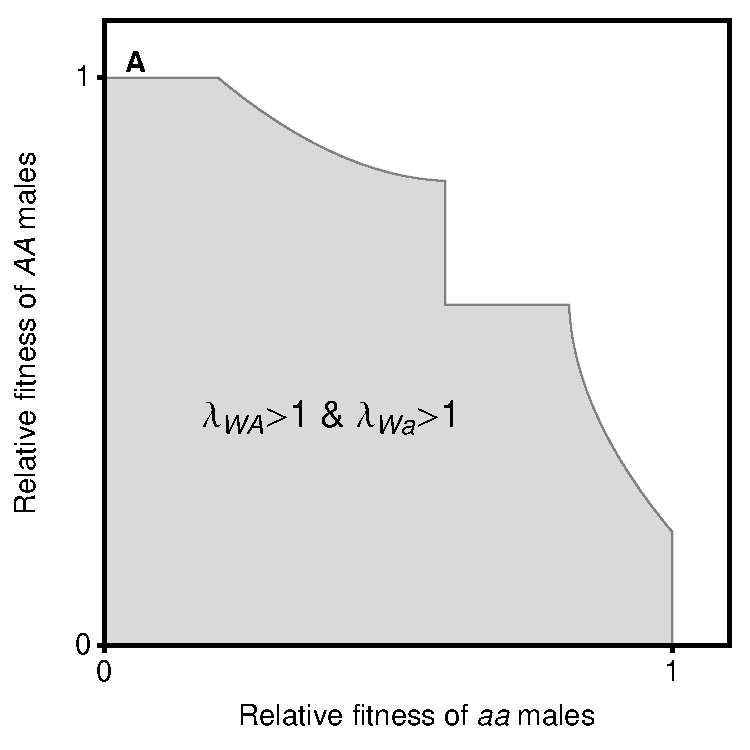
\includegraphics[width=0.45\linewidth]{regionplot_2a}
%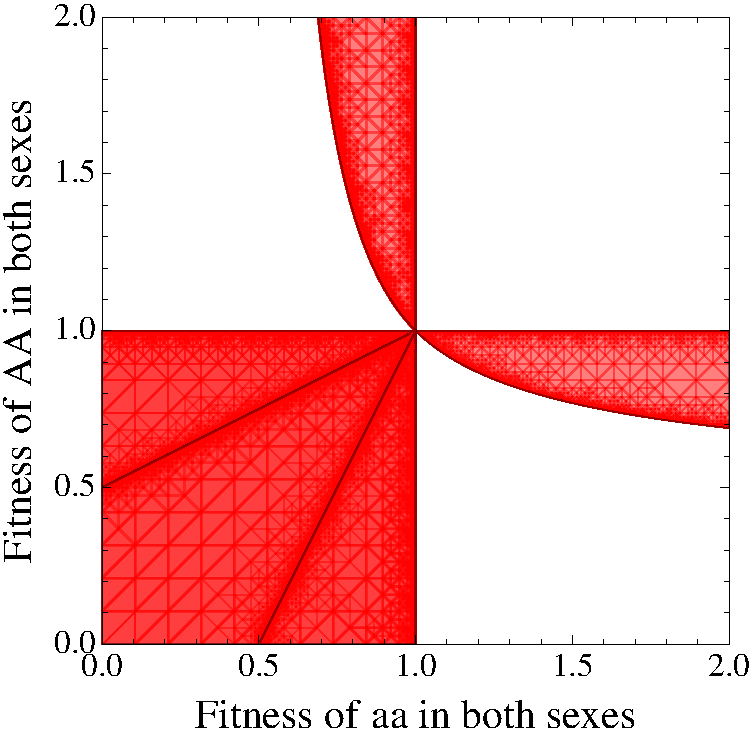
\includegraphics[width=0.45\linewidth]{regionplot_3}\\
%\caption{
%Numerical exploration of where sex-specialist (red) and perverse (blue) hypotheses are valid, i.e., where an internally stable resident equilibrium can be invaded by a neo-W that is perfectly linked with the allele not fixed on the Y (red) or the allele that is fixed on the Y (blue). 
%\textbf{(Left)}
%The perverse equilibrium is only valid with overdominance while the sex-specialist hypothesis is valid over the entire range shown.
%Both hypotheses are simultaneously valid over much of the parameter space where increased recombination between the sex chromosomes is selected \citep[][figure 2a]{Otto2014}.
%\textbf{(Right)}
%Only the sex-specialist hypothesis is valid with no sex-differences in selection, despite selection for increased recombination between the sex-chromosomes with strong overdominance \citep[][figure 3]{Otto2014}.
%Parameters: $w_{Aa}^\Hermaphrodite = 1$, $w_a^\Hermaphrodite = w_A^\Hermaphrodite = 1$, $\alpha^\Hermaphrodite = 1/2$, $r=R=0$, and in left panel $w_{aa}^\female = w_{AA}^\female = 0.6$.
%}
%\label{fig:Region_Plots}
%\end{figure}
%%%%%%%%%%%%%%%%%%%%%%%%%%%%%%%%%%%%%%%%%%%%%%%%%%%%%%%%%


\section*{Supplementary Figures}

%%%%%%%%%%%%%%%%%%%%%%%%%%%%%%%%%%%%%%%%%%%%%%%%%%%%%%%%%
%Both neo-W haplotypes can spread, in the absence of haploid selection, when there is overdominance
%%%%%%%%%%%%%%%%%%%%%%%%%%%%%%%%%%%%%%%%%%%%%%%%%%%%%%%%%
\begin{figure}[!h]
\centering
\centerline{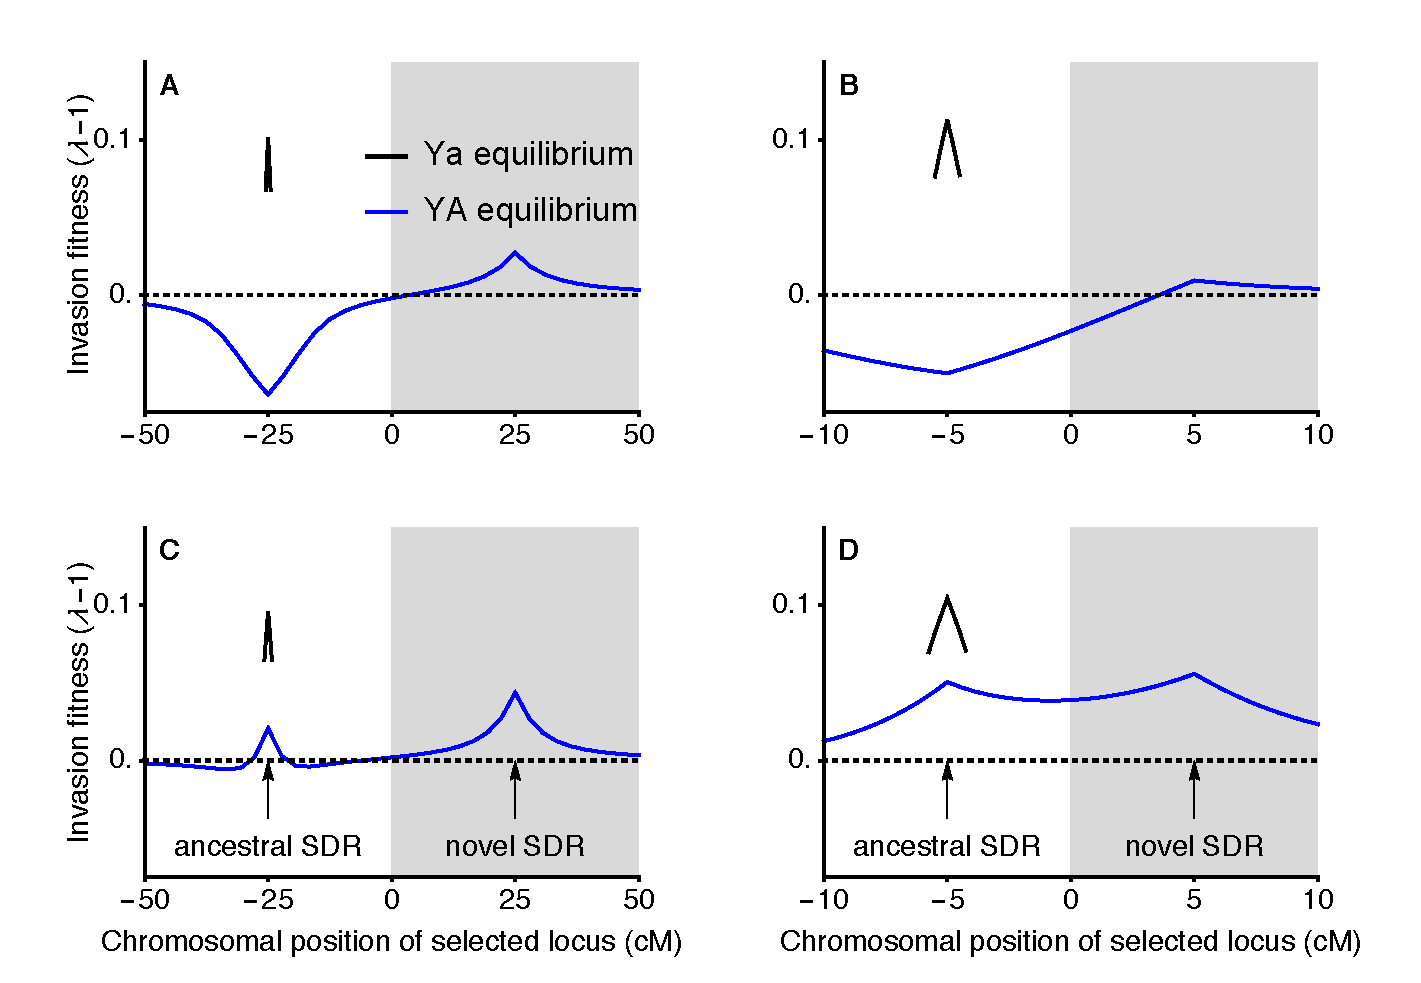
\includegraphics[width=\linewidth]{PositionPlot_Overdominance_Mike}}
\caption{
Neo-W alleles can spread when loci under diploid selection are tightly linked to the ancestral sex determining locus ($r\approx0$). 
In panels A and B, the $a$ allele is favoured in females ($w_{aa}^\female=1.05$, $w_{Aa}^\Hermaphrodite=1$, $w_{AA}^\female=0.85$) and selection in males is overdominant ($w_{aa}^\male=w_{AA}^\male=0.75$).
In panels C and D, selection in males and females is overdominant ($w_{aa}^\female=w_{AA}^\female=0.6$, $w_{aa}^\male=0.5$, $w_{AA}^\male=0.7$, $w_{Aa}^\Hermaphrodite=1$).
There is no haploid selection $t^\Hermaphrodite = \alpha^\Hermaphrodite_\Delta = 0$.
These parameters are marked by daggers in Figure \ref{fig:regionplots}B and C, which show that neo-W invasion is expected for any $R$ ($\lambda_{WA},\lambda_{Wa}>1$) when the $a$ allele is nearly fixed on the Y (black lines in this figure). 
Equilibria where the $A$ allele is more common among Y-bearing male gametes can also be stable and allow neo-W invasion for these parameters (blue lines). 
The weak selection approximation holds when all recombination rates are large relative to selection (around 0 in panels A and C), in which case, in the absence of haploid selection, neo-W alleles should spread only if they are more tightly linked to the selected locus (positive invasion fitness if and only if the selected locus is in the grey region). 
However, when linkage is tight (panels C and D and when the selected locus is near the SDR in all panels), this prediction breaks down. 
}
\label{fig:positionOverdominance}
\end{figure}

\newpage

%%%%%%%%%%%%%%%%%%%%%%%%%%%%%%%%%%%%%%%%%%%%%%%%%%%%%%%%%
%Both neo-W haplotypes can spread, in the absence of haploid selection, when there is overdominance
%%%%%%%%%%%%%%%%%%%%%%%%%%%%%%%%%%%%%%%%%%%%%%%%%%%%%%%%%
\begin{figure}[!h]
\centering
\centerline{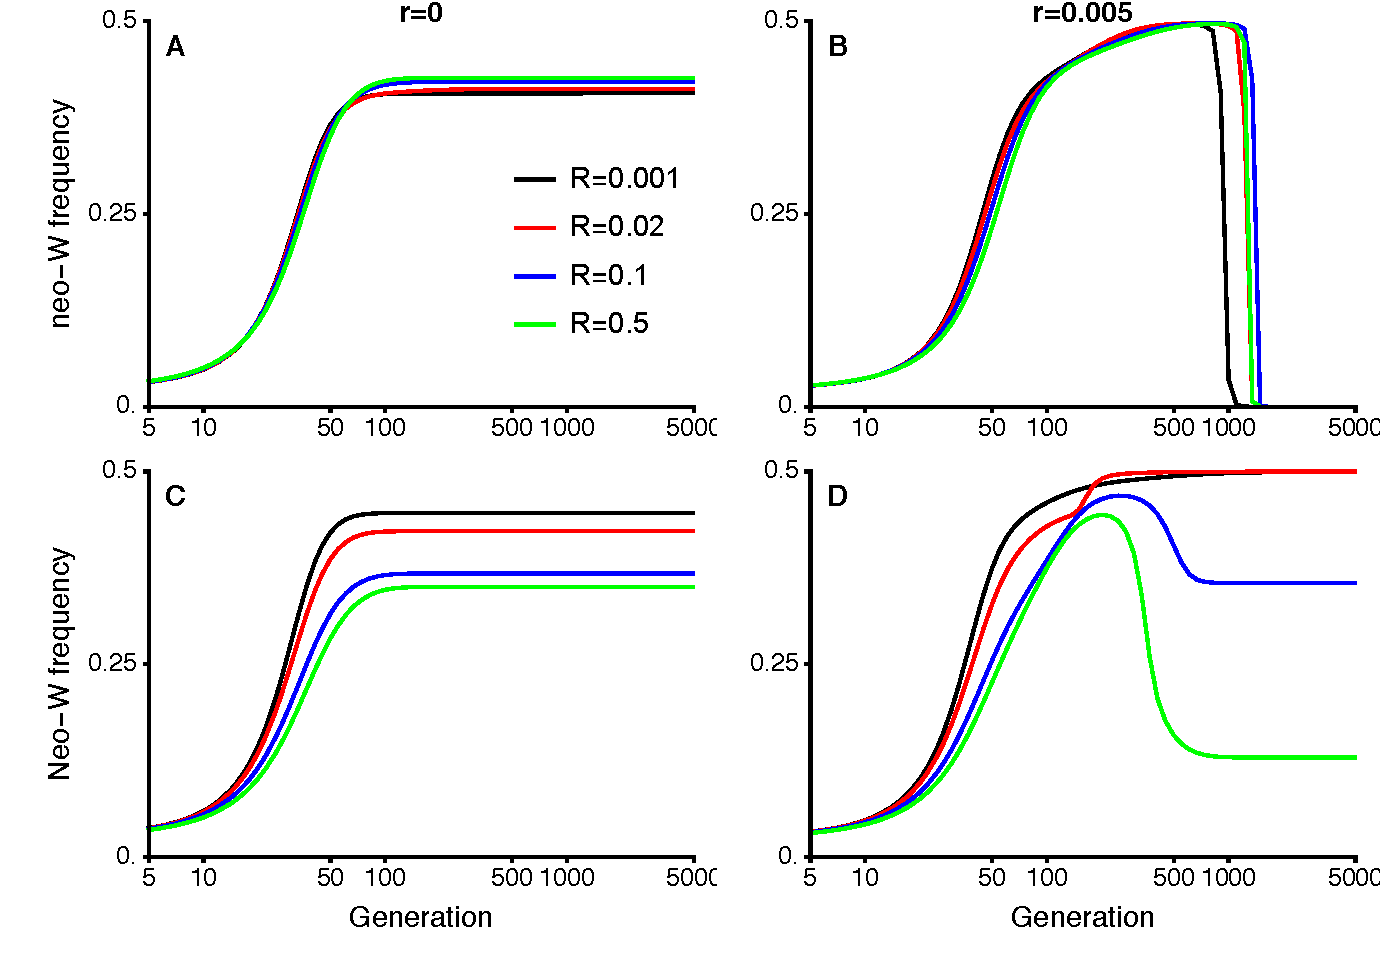
\includegraphics[width=\linewidth]{Temporal_Overdominance_Mike}}
\caption{
Following invasion by a neo-W allele, there can be a complete transition to a new sex-determination system, maintenance of polymorphism at both ancestral-XY and neo-ZW sex determining regions, or loss of the new sex-determining allele. 
Here we plot the frequency of the neo-W allele among female gametes; as the neo-W reaches frequency $0.5$, polymorphism at the ancestral XY locus is lost with Y becoming fixed such that sex is determined only be the ZW allele carried by a female gamete. 
Panels A, C and D show cases where a steady state is reached with the neo-W at a frequency below $0.5$, in which case ancestral-X and Y alleles also both segregate. 
In all cases, we assume that the $a$ allele is initially more common that the $A$ allele on the Y (Y-$a$ is fixed when $r=0$). 
When $r>0$ (panels B and D), Y-$A$ haplotypes created by recombination can become more common than Y-$a$ haplotypes as the neo-W spreads.
In B, this leads to loss of the neo-W and the system goes to an equilibrium with X-$a$ and Y-$A$ haplotypes fixed (A'), such that all females have the high fitness genotype $aa$ and all males $Aa$. 
For the parameters in B, neo-W alleles have negative invasion fitness when the Y-$A$ haplotype is ancestrally more common than Y-$a$ (see blue line in Figure \ref{fig:temporalOverdominance}A and  \ref{fig:temporalOverdominance}B). 
In contrast, the neo-W is not lost in panel D (see blue line in Figure \ref{fig:temporalOverdominance}C and  \ref{fig:temporalOverdominance}D). 
Fitness parameters are the same as in Figure \ref{fig:temporalOverdominance}, the $a$ allele is favoured in females ($w_{aa}^\female=1.05$, $w_{Aa}^\Hermaphrodite=1$, $w_{AA}^\female=0.85$) and there is overdominant selection in males ($w_{aa}^\male=w_{AA}^\male=0.75$) in panels A and B.
In panels C and D, selection in males and females is overdominant ($w_{aa}^\female=w_{AA}^\female=0.6$, $w_{aa}^\male=0.5$, $w_{AA}^\male=0.7$, $w_{Aa}^\Hermaphrodite=1$). 
These parameters are marked by a dagger in Figure \ref{fig:regionplots}. 
Here, there is no haploid selection $t^\Hermaphrodite = \alpha^\Hermaphrodite_\Delta = 0$.
}
\label{fig:temporalOverdominance}
\end{figure}

\begin{figure}[!h]
\centering
\centerline{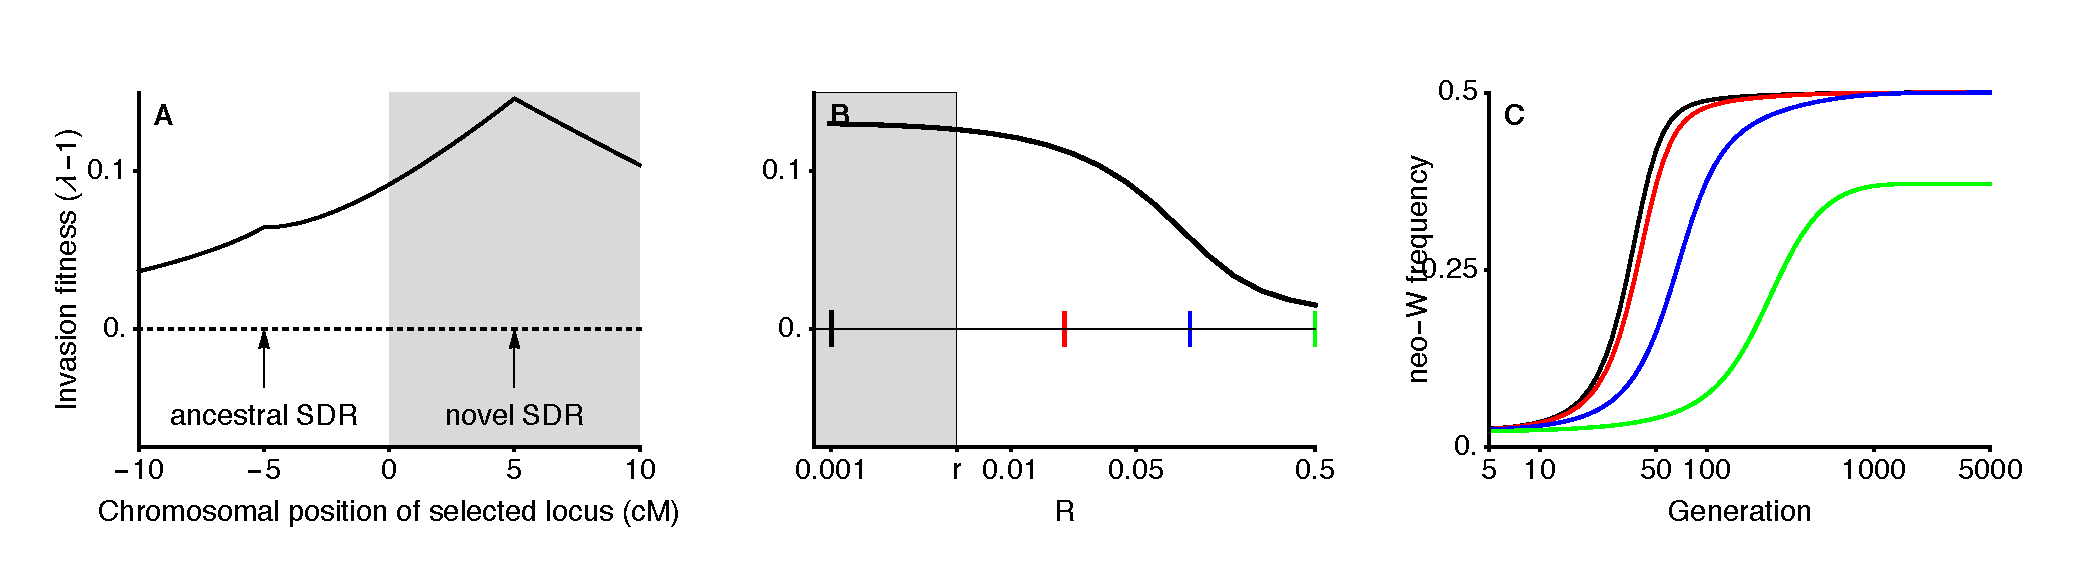
\includegraphics[width=1.5\linewidth]{PositionPlot_SexAntagTighter_MaleDrive_Mike}}
\caption{
When there is sexually-antagonistic selection and haploid selection, a neo-W may invade for any $R$.
Panel A shows that the invasion fitness of a neo-W is positive where linkage is tight, even when $r<R$ (unshaded region). \textcolor{red}{(remove A?)}
In panel B, we vary the recombination rate between the neo-W and the selected locus ($R$) for a fixed recombination rate between the ancestral-SDR and the selected locus ($r=0.005$).
Coloured markers show recombination rates for which the temporal dynamics of neo-W invasion are plotted in panel C (black $R=0.001$, red $R=0.02$, blue $R=0.1$, green $R=0.5$). 
The diploid selection parameters used in this plot are the same as in Figure \ref{fig:SexAntagTighter}, marked by an asterisk in Figure \ref{fig:regionMaleDrive}A: $w_{AA}^\female=1.05$, $w_{Aa}^\Hermaphrodite=1$, $w_{aa}^\female=0.85$, $w_{AA}^\male=0.85$, $w_{aa}^\male=1.05$, $\alpha_{\Delta}^\male=-0.08$, except that there is also male meiotic drive in favour of the $a$ allele, $\alpha_{\Delta}^\male=-0.08$.
When $R=0.5$ (green curve), the neo-W does not reach fixation and X,Y,Z, and W alleles are all maintained in the population, see Figure \ref{fig:freqAll}C.
}
\label{fig:SexAntagTighterMaleDrive}
\end{figure}

\begin{figure}[!h]
\centering
\centerline{\includegraphics[width=\linewidth]{Region_Plot_combined_MaleDrive_Mike}}
\caption{
Meiotic drive in males affects whether neo-W-$A$ and neo-W-$a$ haplotypes spread when the ancestral-XY locus is tightly linked to a locus under selection ($r=0$). 
We vary the fitness of male homozygotes relative to heterozygotes ($w_{Aa}^\Hermaphrodite=1$) and only consider stable equilibria at which both \textbf{A} locus allele are maintained and the $a$ allele is initially fixed on the Y, region outlined. 
In panels A-C, meiotic drive in males favours the $a$ allele ($\alpha_{\Delta}^\male=-0.16$), creating male-biased sex ratios and generally increasing $\lambda_{WA}$ and $\lambda_{Wa}$. 
By contrast, $\lambda_{WA}$ and $\lambda_{Wa}$ tend to be reduced when meiotic drive in males favours the $A$ allele ($\alpha_{\Delta}^\male=0.16$), panels D-F. 
We consider three forms of selection in females: directional selection in favour of the $A$ allele (panels A and D, $w_{aa}^\female=0.85$, $w_{AA}^\female=1.05$), direction selection in favour of the $a$ allele (panels B and E, $w_{aa}^\female=1.05$, $w_{AA}^\female=0.85$), and overdominance (panels C and F, $w_{aa}^\female=0.6$, $w_{AA}^\female=0.6$).
%\textcolor{red}{Panel F mislabelled, should have $\lambda_{Wa}>1$ \& $\lambda_{WA}<1$ as the upper label that has the line.}
}
\label{fig:regionMaleDrive}
\end{figure}

\newpage
\begin{figure}[!h]
\centering
\centerline{\includegraphics[width=\linewidth]{Region_Plot_combined_MaleGS_Mike}}
\caption{
Parameters for which neo-W-$A$ and neo-W-$a$ haplotypes spread when there is male gametic competition at a locus that is tightly linked to the ancestral-XY locus.
Diploid selection parameters ($w_{ij}^\Hermaphrodite$) are the same as those in Figure \ref{fig:regionMaleDrive}. 
The $a$ allele is favoured during male gametic competition in Panels A-C ($w_{a}^\male=1.16$, $w_{A}^\male=1$), which creates male biased sex-ratios and increases $\lambda_{WA}$ and $\lambda_{Wa}$. 
On the other hand, the $A$ allele is favoured during male gametic competition in Panels D-F ($w_{a}^\male=1$, $w_{A}^\male=1.16$) and $\lambda_{WA}$ and $\lambda_{Wa}$ tend to be reduced. 
Compared to the meiotic drive parameters in Figure \ref{fig:regionMaleDrive}, the effect of these male gametic competition parameters on the sex ratio is smaller. 
For example, in Figure \ref{fig:regionMaleDrive}A-C, the ancestral sex ratio is $\alpha^\male=0.58$ at equilibrium (B) and in panels A-C of this plot, the ancestral sex ratio is $w_{a}^\male/(w_{A}^\male+w_{a}^\male)=0.537$ at equilibrium (B). 
}
\label{fig:regionMaleGS}
\end{figure}

\begin{figure}[!h]
\centering
\centerline{\includegraphics[width=\linewidth]{Region_Plot_combined_FemaleDrive_Mike}}
\caption{
Parameters for which neo-W-$A$ and neo-W-$a$ haplotypes spread when there is female meiotic drive at a locus that is tightly linked to the ancestral-XY locus.
Diploid selection parameters ($w_{ij}^\Hermaphrodite$) are the same as those in Figure \ref{fig:regionMaleDrive} and \ref{fig:regionMaleGS}. 
The $a$ allele is favoured by meiotic drive in females in Panels A-C ($\alpha_{\Delta}^\female=-0.16$), which increases $\lambda_{Wa}$ and decreases $\lambda_{WA}$. 
Female meiotic drive in favour of the $A$ allele (panels D-F, $\alpha_{\Delta}^\female=-0.16$) has the opposite effect. 
}
\label{fig:regionFemaleDrive}
\end{figure}

\begin{figure}[!h]
\centering
\centerline{\includegraphics[width=\linewidth]{Region_Plot_combined_FemaleGS_Mike}}
\caption{
Parameters for which neo-W-$A$ and neo-W-$a$ haplotypes spread when there is female meiotic drive at a locus that is tightly linked to the ancestral-XY locus.
Diploid selection parameters ($w_{ij}^\Hermaphrodite$) are the same as those in Figure \ref{fig:regionMaleDrive}, \ref{fig:regionMaleGS}, and \ref{fig:regionFemaleDrive}. 
The $a$ allele is favoured during female gametic competition in females in Panels A-C ($\alpha_{\Delta}^\female=-0.16$), which increases $\lambda_{Wa}$ and decreases $\lambda_{WA}$. 
The $A$ allele is favoured during gametic competition in panels D-F ($\alpha_{\Delta}^\female=-0.16$), giving the opposite effect on $\lambda_{Wa}$ and $\lambda_{WA}$. 
}
\label{fig:regionFemaleGS}
\end{figure}

\begin{landscape}
\begin{figure}[!h]
\centering
\centerline{
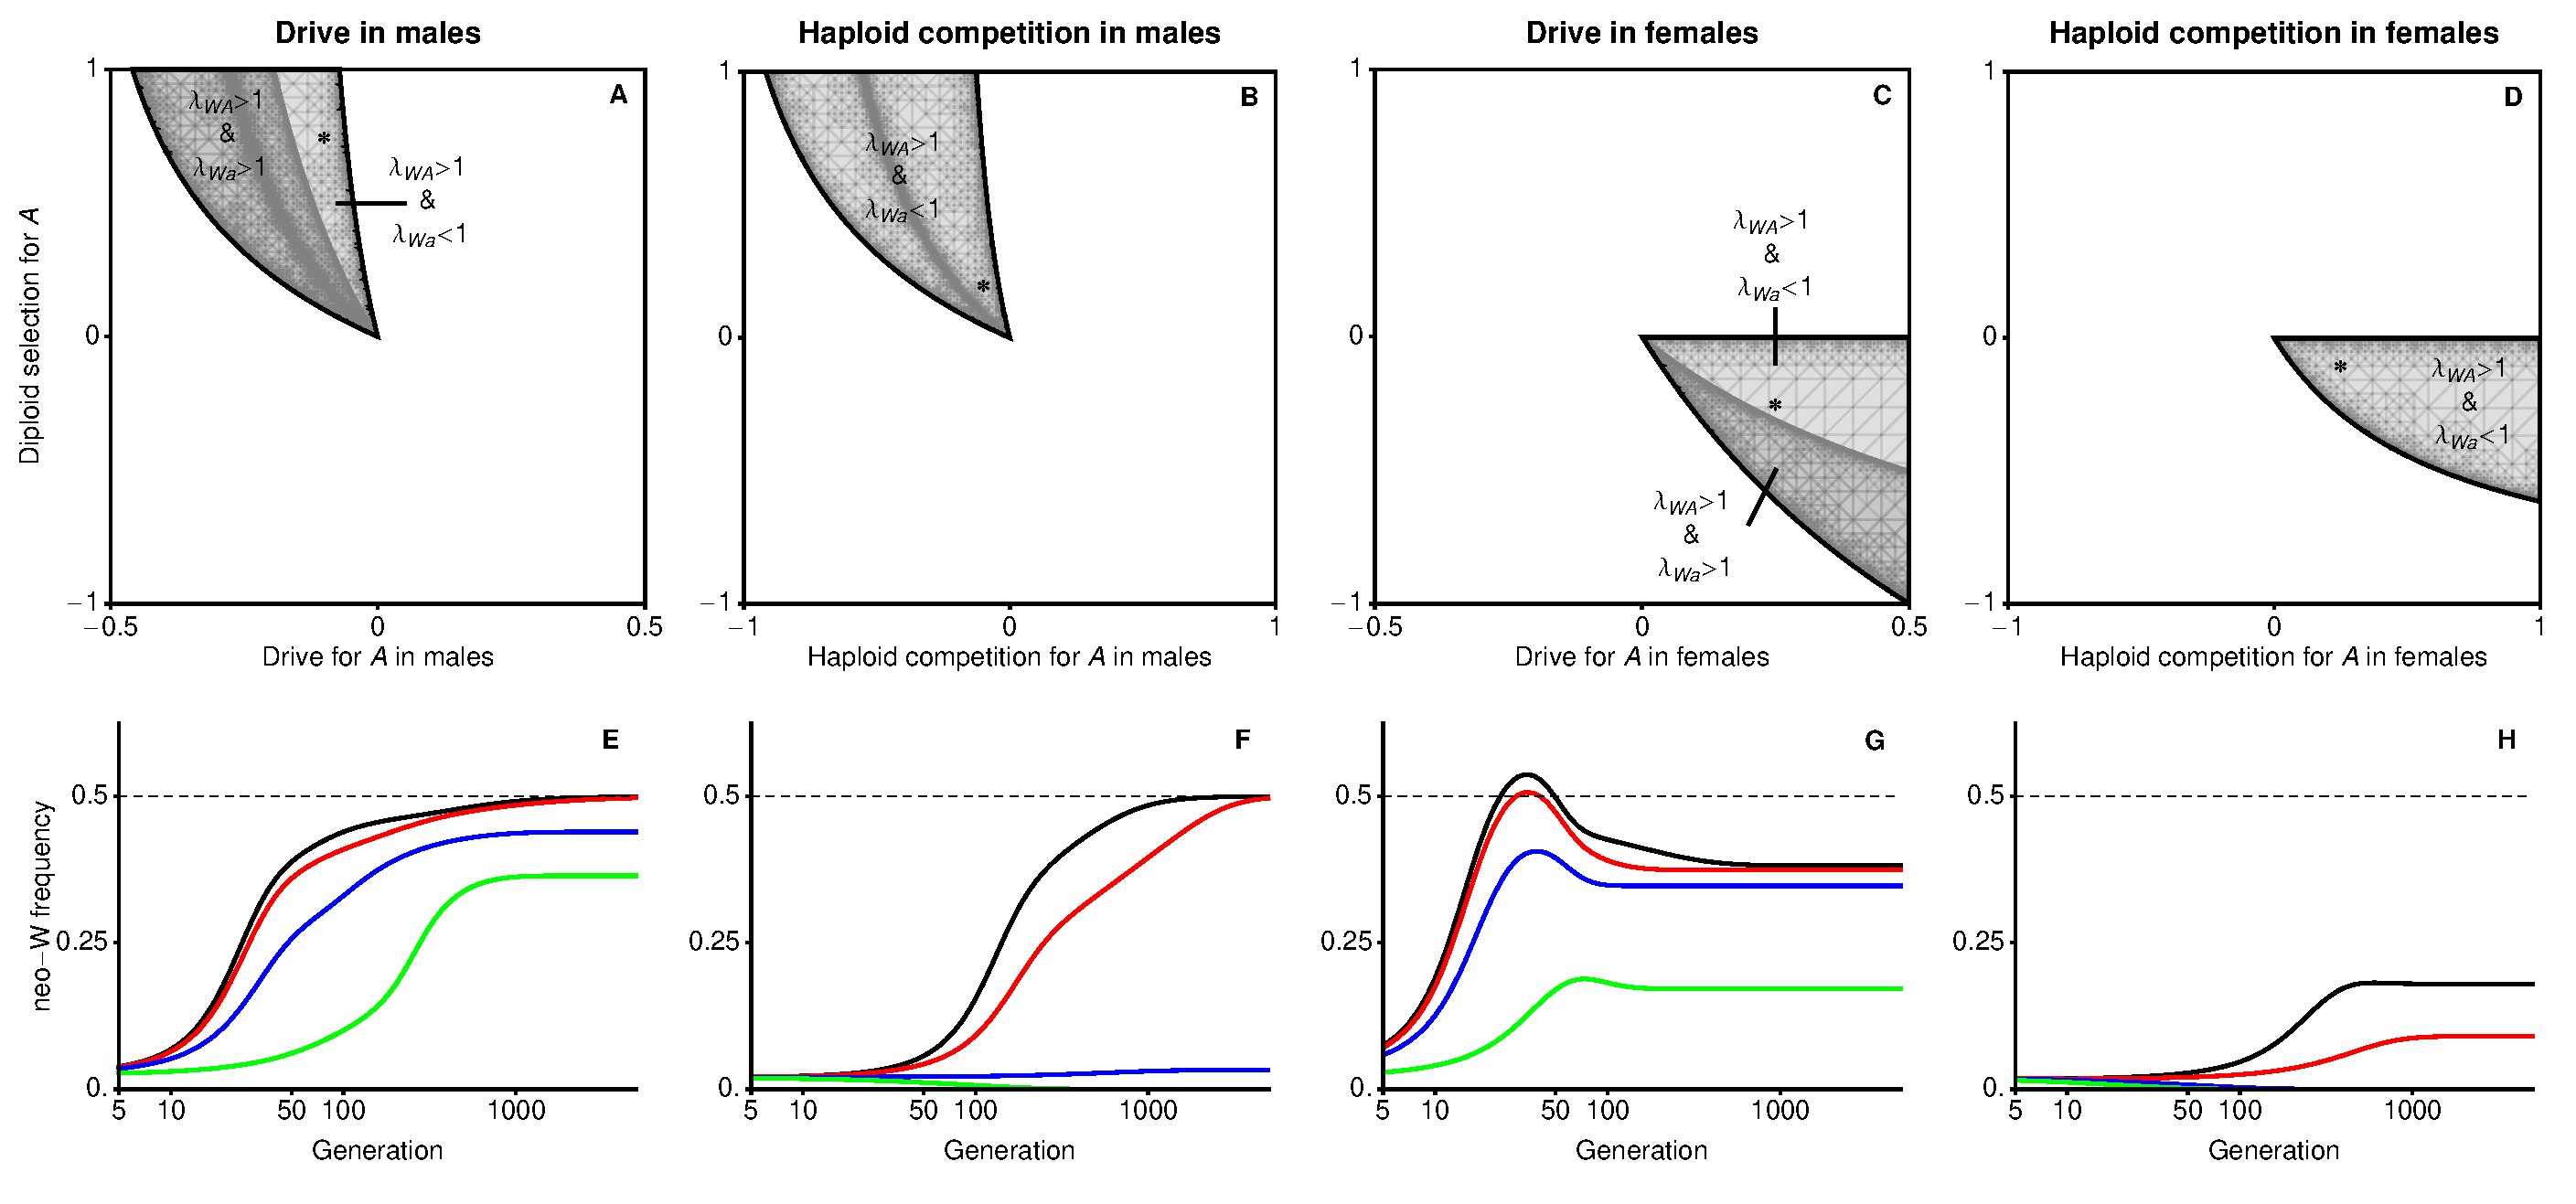
\includegraphics[width=\linewidth]{All_plot_combined_PloidAntag_Matt}
}
\caption{
A-D show when each of the neo-W haplotypes invade an internally stable equilibrium with $a$ fixed on the Y (found by setting $r=0$).
The y-axis shows directional selection in diploids of both sexes, $s^\female=s^\male$, and the x-axes show sex-specific drive, $\alpha_\Delta^\Hermaphrodite$, or haploid competition, $t^\Hermaphrodite$.
The top left and bottom right quadrants therefore imply ploidally-antagonistic selection (and these are the only places where neo-W haplotypes can invade).
Dominance is equal in both sexes, $h^\female=h^\male=3/4$. 
E-F show the temporal dynamics of neo-W frequency in females with parameters given by the asterisks in the corresponding A-D plot, with $r=1/200$, for four different $R$.
Black $R=1/1000$, Red $R=2/100$, Blue $R=1/10$, Green $R=1/2$.  
Dashed line in E-H gives ``fixation" of neo-W (all females heterozygous ZW).
}
\label{fig:regionPloidAntag}
\end{figure}
\end{landscape}

\begin{landscape}
\begin{figure}[!h]
\centering
\centerline{
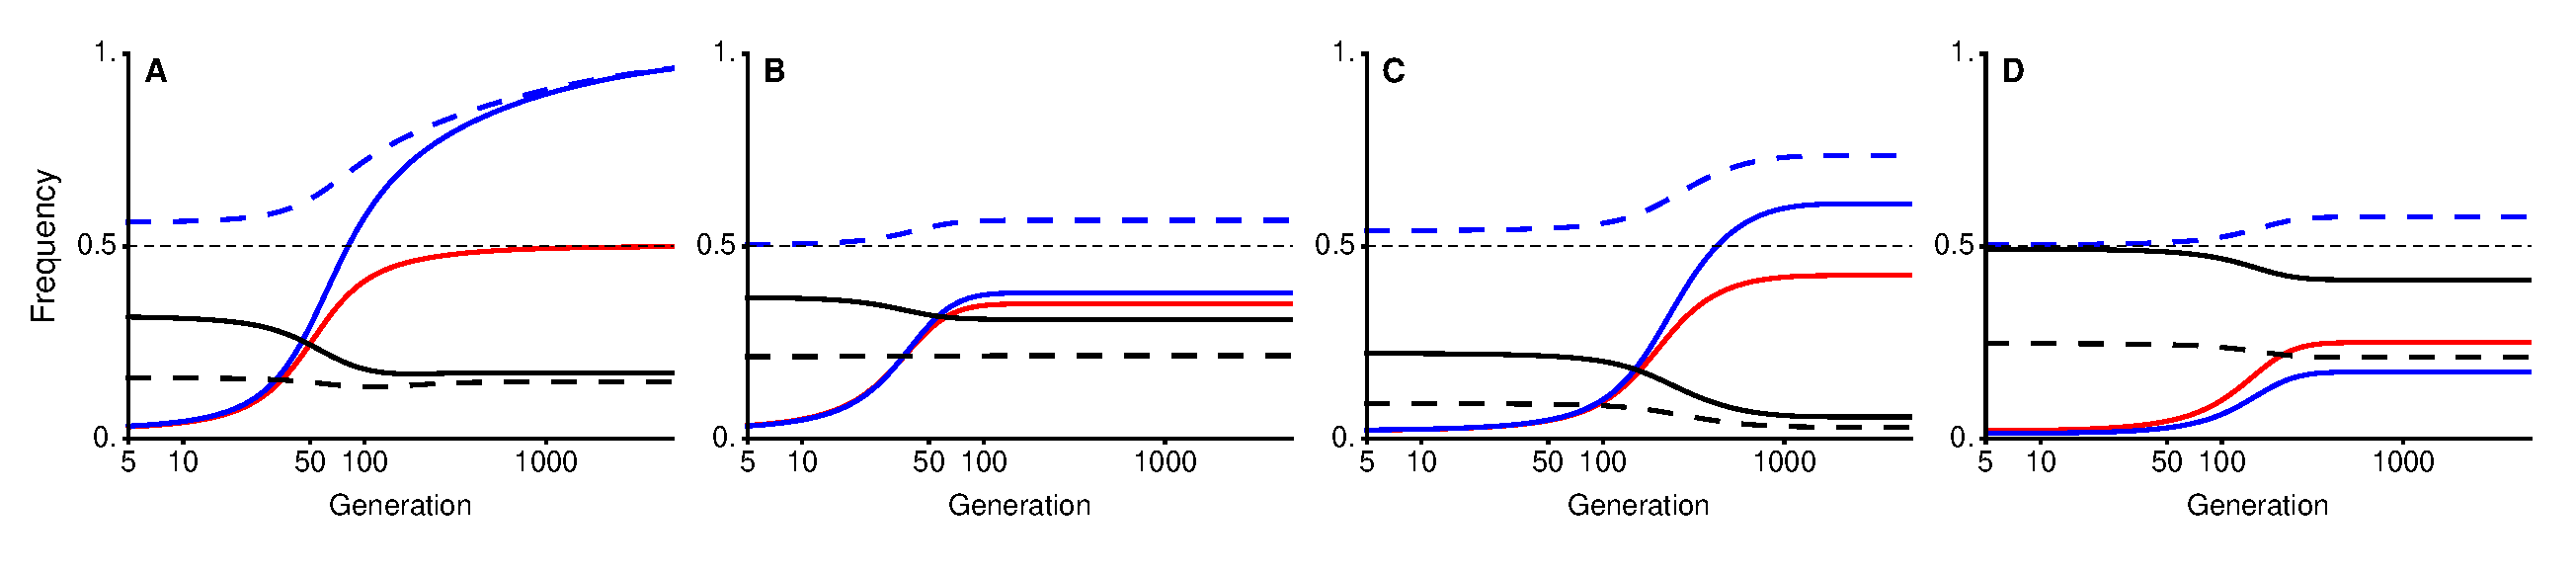
\includegraphics[width=\linewidth]{Freq_plot_combined_PloidAntag_Matt}
}
\caption{
Dynamics of sex-determining alleles during invasion by a neo-W allele. 
The curves show the frequencies of the neo-W (red), ancestral-Y (Blue), and $A$ allele among female gametes (solid curves) and among male gametes (dashed curves). 
In panel A, there is a complete transition from XY sex determination (XX-ZZ females and XY-ZZ males) to ZW sex determination (YY-ZW females and YY-ZZ males).  
In panels B-D polymorphism is maintained at both the ancestral XY locus and the neo-ZW locus, such that there are males with genotypes XY-ZZ or YY-ZZ and females with genotypes XX-ZZ, XX-ZW, XY-ZW, or YY-ZW. 
In panel A, selection is ploidally antagonistic with drive in males (parameters as in the green curve in Figure \ref{fig:SexRatioBad}B).
In panel B, there is overdominance in both sexes (parameters as the green curve in Figure \ref{fig:temporalOverdominance}C).
In panel C, there is male meiotic drive and sexually-antagonistic selection in diploids (parameters as the green curve in Figure \ref{fig:regionMaleDrive}C).
\textcolor{red}{(remove D?)}
Panel D has the same parameters as the red curve in Figure \ref{fig:regionPloidAntag}F, except $r=0$ (ploidy-antagonism with pollen competition).
In all cases, the initial equilibrium frequency has $a$ near fixed on the Y.
}
\label{fig:freqAll}
\end{figure}
\end{landscape}

%\begin{figure}[!h]
%\centering
%\centerline{
%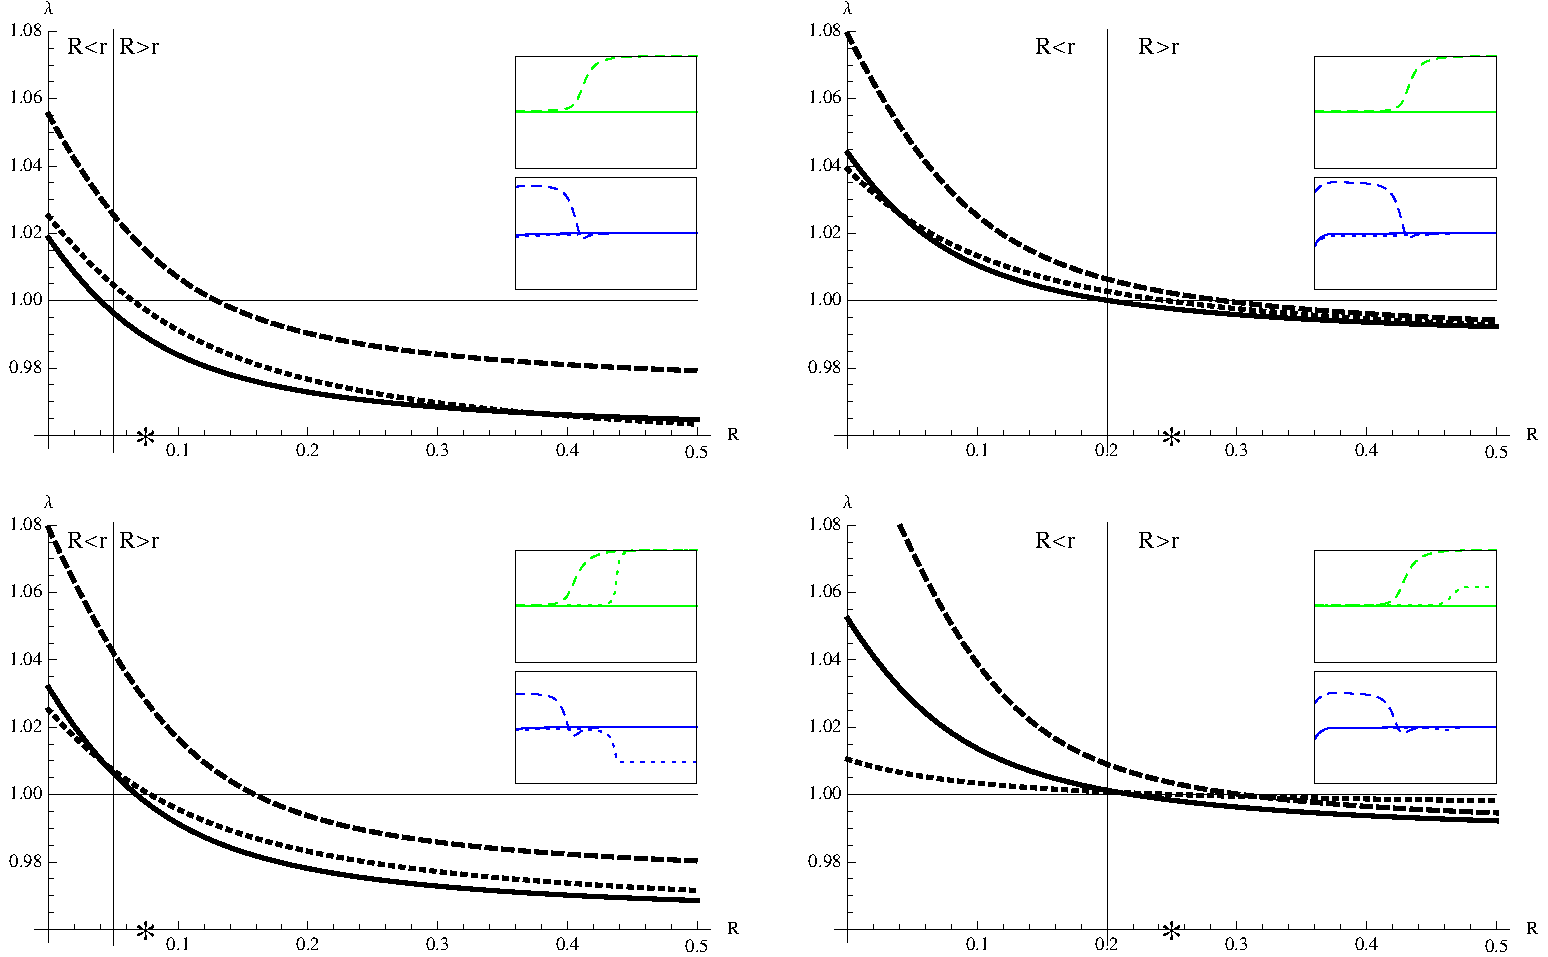
\includegraphics[width=\linewidth]{Sallys_R_plot.pdf}
%}
%\caption{
%\textcolor{blue}{is this the one?}
%}
%\label{fig:lambda_R}
%\end{figure}

%\newpage
%\textcolor{red}{
%Add Sally's figure showing lambda for small r near equil A versus near equil B. Add references to this figure to appendix where we discuss whether lambdas can be greater than 1 with sexually antagonistic selection.}
%\textcolor{blue}{not sure which one you are talking about, but see Figure \ref{fig:lambda_R} }
%\textcolor{red}{Let's remove this for now.}

%\textcolor{red}{
%Perhaps it would also be useful to add an 8 panel figure that features ploidally antagonistic selection. For each type of haploid selection (gametic competition/ meiotic drive in males/females), give a regionplot where $h^\male=h^\female$, e.g., $h^\male=h^\female=0.75$ (or perhaps the value of $h$ we use in the regionplots we have, in which $w_{aa}=0.85$, $w_{Aa}=1$, $w_{AA}=1.05$). 
%Matt made a figure like this before but both Y$a$ and Y$A$ equilibria were plotted and there was no outline showing where the Y$a$ equilibrium is stable (as in Figure \ref{fig:regionplots}). In Matts plot the axes were $s^\Hermaphrodite$ and $\alpha_{\Delta}^\Hermaphrodite$. 
%Add an asterisk to each region plot and show invasion in another panel, using those parameters and various $R$ (e.g., in the stye of \ref{fig:temporalOverdominance}). 
%In an email, Sally has an example of ploidally-antagonistic selection where the neo-W fixes and $R=1/2$. This would cover that case and more. }
%\textcolor{blue}{made an attempt (Figure \ref{fig:regionPloidAntag})}

%\textcolor{red}{
%We could also give versions of Figure \ref{fig:regionplots} where there is also haploid selection of various types.
%Haploid selection can favour $A$ or $a$, so this would involve 4x 6-panel figures. Started looking at this in Figure \ref{fig:regionMaleGS} and Figure \ref{fig:regionMaleDrive}, add female haploid selection. 
%Try to integrate into the discussion of haploid selection? e.g., male haploid selection ones generally show effect of sex ratio, increasing both lambdas when female biased (top rows).}
%\textcolor{blue}{
%these figures are now done (\ref{fig:regionMaleDrive}-\ref{fig:regionFemaleGS}) (ensuring frequencies between 0 and 1), but yet to discuss in text.}

%\textcolor{red}{
%Perhaps, for one set of parameters, we should plot the dynamics of all the different alleles. E.g., we could use the same parameters used in \ref{fig:SexRatioBad}. The main purpose would be to show what happens to the ancestral SDR during turnover. 
%We could also show an example where XY and ZW sex determining systems are both polymorphic and stable (e.g., using one of the curves in Figure \ref{fig:temporalOverdominance} and the green curve in Figure \ref{fig:SexAntagTighterMaleDrive}). 
%I think there are also examples with looser sex linkage and pollen competition that lead to a mixed sex-determination system. We should probably have a short section in the appendix discussing this. }
%\textcolor{blue}{made an attempt with Figure \ref{fig:freqAll}, but yet to discuss in text}


\end{document}



